% LaTEX source code
% Last modified November 1st, 2005
% Steve Miller
% note that the percent sign comments out the rest of the line
% first, we set a document class. often use 12pt characters, though
% sometimes people do 11 or 10. you can do report or article, both similar
%\documentclass[12pt,letterpaper]{article}
\documentclass[12pt,reqno]{amsart}
\linespread{1}
\addtolength{\textwidth}{2cm} \addtolength{\hoffset}{-1cm}
\addtolength{\marginparwidth}{-1cm} \addtolength{\textheight}{2cm}
\addtolength{\voffset}{-1cm}
% below are some packages that are needed for certain symbols, graphics, colors.
% safest to just include these.
\usepackage{times}
\usepackage[T1]{fontenc}
\usepackage{mathrsfs}
\usepackage{latexsym}
\usepackage[dvips]{graphics}
\usepackage{epsfig}
\usepackage{hyperref, amsmath, amsthm, amsfonts, amscd, flafter,epsf}
\usepackage{amsmath,amsfonts,amsthm,amssymb,amscd}
\input amssym.def
\input amssym.tex
\usepackage{color}
\usepackage{enumerate}
\usepackage{hyperref}
\usepackage{url}
\usepackage{floatrow}
\usepackage{caption}
\usepackage{subcaption}
\usepackage{capt-of}
\usepackage{physics}
\newcommand{\todo}[1]{\textcolor{red}{\textbf{(#1)}}}

    %=======================================================

    %   THIS IS WHERE YOU PUT SHORTCUT DEFINITIONS

    %========================================================

% Note that we use a percent sign to comment out a line

% below are shortcut commands

%%%%%%%%%%%%%%%%%%%%%%%%%%%%%%%%%%%%%%%%%%%%%%%

% below are shortcuts for equation, eqnarray,

% itemize and enumerate environments

\newcommand\be{\begin{equation}}
\newcommand\ee{\end{equation}}
\newcommand\bea{\begin{eqnarray}}
\newcommand\eea{\end{eqnarray}}
\newcommand\bi{\begin{itemize}}
\newcommand\ei{\end{itemize}}
\newcommand\ben{\begin{enumerate}}
\newcommand\een{\end{enumerate}}
\newcommand{\ncr}[2]{\left({#1 \atop #2}\right)}
%%%%%%%%%%%%%%%%%%%%%%%%%%%%%%%%%%%%%%%%%%%%%%%%

% Theorem / Lemmas et cetera

\newtheorem{thm}{Theorem}[section]
\newtheorem{conj}[thm]{Conjecture}
\newtheorem{cor}[thm]{Corollary}
\newtheorem{lem}[thm]{Lemma}
\newtheorem{prop}[thm]{Proposition}
\newtheorem{exa}[thm]{Example}
\newtheorem{defi}[thm]{Definition}
\newtheorem{exe}[thm]{Exercise}
\newtheorem{rek}[thm]{Remark}
\newtheorem{que}[thm]{Question}
\newtheorem{prob}[thm]{Problem}
\newtheorem{cla}[thm]{Claim}
\newtheorem{defis}[thm]{Definitions}
\newtheorem{res}[thm]{Result}
\newtheorem{calc}[thm]{Calculation}
%%%%%%%%%%%%%%%%%%%%%%%%%%%%%%%%%%%%%%%%%

% shortcuts to environments

% this allows you to do textboldface: simply type \tbf{what you want in bold}

\newcommand{\tbf}[1]{\textbf{#1}}

%%%%%%%%%%%%%%%%%%%%%%%%%%%%%%%%%%%%%%%%%%%%%%%%%%

% shortcut to twocase and threecase definitions

\newcommand{\twocase}[5]{#1 \begin{cases} #2 & \text{#3}\\ #4
&\text{#5} \end{cases}   }
\newcommand{\threecase}[7]{#1 \begin{cases} #2 &
\text{#3}\\ #4 &\text{#5}\\ #6 &\text{#7} \end{cases}   }
%%%%%%%%%%%%%%%%%%%%%%%%%%%%%%%%%%%%%%%%%

%Blackboard Letters

\newcommand{\R}{\ensuremath{\mathbb{R}}}
\newcommand{\C}{\ensuremath{\mathbb{C}}}
\newcommand{\Z}{\ensuremath{\mathbb{Z}}}
\newcommand{\Q}{\mathbb{Q}}
\newcommand{\N}{\mathbb{N}}
\newcommand{\F}{\mathbb{F}}
\newcommand{\W}{\mathbb{W}}
\newcommand{\Qoft}{\mathbb{Q}(t)}  %use in linux
\newcommand{\soln}{\noindent \textbf{Solution:}\ }

%%%%%%%%%%%%%%%%%%%%%%%%%%%%%%%%%%%%%%%%%

% Finite Fields and Groups

\newcommand{\Fp}{ \F_p }
%%%%%%%%%%%%%%%%%%%%%%%%%%%%%%%%%%%%%%%%%

% Fractions

\newcommand{\foh}{\frac{1}{2}}  %onehalf
\newcommand{\fot}{\frac{1}{3}}
\newcommand{\fof}{\frac{1}{4}}

%%%%%%%%%%%%%%%%%%%%%%%%%%%%%%%%%%%%%%%%%

% Legendre Symbols

\newcommand{\js}[1]{ { \underline{#1} \choose p} }

%%%%%%%%%%%%%%%%%%%%%%%%%%%%%%%%%%%%%%%%%

% matrix shortcuts

\newcommand{\mattwo}[4]
{\left(\begin{array}{cc}
                        #1  & #2   \\
                        #3 &  #4
                          \end{array}\right) }
\newcommand{\matthree}[9]
{\left(\begin{array}{ccc}
                        #1  & #2 & #3  \\
                        #4 &  #5 & #6 \\
                        #7 &  #8 & #9
                          \end{array}\right) }
\newcommand{\dettwo}[4]
{\left|\begin{array}{cc}
                        #1  & #2   \\
                        #3 &  #4
                          \end{array}\right| }
\newcommand{\detthree}[9]
{\left|\begin{array}{ccc}
                        #1  & #2 & #3  \\
                        #4 &  #5 & #6 \\
                        #7 &  #8 & #9
                          \end{array}\right| }
%%%%%%%%%%%%%%%%%%%%%%%%%%%%%%%%%%%%%%%%%

% greek letter shortcuts

\newcommand{\ga}{\alpha}                  %gives you a greek alpha
\newcommand{\gb}{\beta}
\newcommand{\gep}{\epsilon}
%%%%%%%%%%%%%%%%%%%%%%%%%%%%%%%%%%%%%%%%%

% general functions

\newcommand{\notdiv}{\nmid}               % gives the not divide symbol
\newcommand{\burl}[1]{\textcolor{blue}{\url{#1}}}

%%%%%%%%%%%%%%%%%%%%%%%%%%%%%%%%%%%%%%%%%%%

% the following makes the numbering start with 1 in each section;

% if you want the equations numbered 1 to N (without caring about

% what section you are in, comment out the following line.

\numberwithin{equation}{section}

%\textwidth= 6in

%\evensidemargin=37pt

%\oddsidemargin=0pt

\begin{document}



\title{Hexane Water Results Log}
\author{Kirk Swanson}
\email{swansonk1@uchicago.edu}
\address{Institute for Molecular Engineering, University of Chicago, 5640 S Ellis Ave, Chicago, IL 60637}
%\keywords{path integral molecular dynamics, path integral monte carlo, metropolis algorithm}
\date{\today}




\maketitle

%%%%%%%%%%%%%%%%%%%%%%%%%%%%%%%%%%%%%%%%%%%%%%%%%%%%%%%%%%%%%%%%%%%%%%%%%%%%%%%%%%%%%%%%%%%%%%%%%%%%%%%%%%%%%%%%%%%%%%%%%%%%%%

\normalsize

%%%%%%%%%%%%%%%%%%%%%%%%%%%%%%%%%%%%%%%%%%%%%%%%%%%%%%%%%%%%%%%%%%%%%%%%%%%%%%%%%%%%%%%%%%%%%%%%%%%%%%%%%%%%%%%%%%%%%%%%%%%%%%

\section{1/8/2018}
\begin{enumerate}
\item Ran a simulation of the hexane-water interface using LAMMPS.  Set up for 1M time steps, but only got through 745,200 due to time limit of 24 hrs.  
\item Ran a simulation of the hexane-water interface in DASH, using the python script "interface.py" in the dash-work/interface folder.  The run was for 4,000,000 time steps, printing a configuration every 50,000 steps.  Below are snapshots of the 0th timestep and the 3,950,000 time step.    

\begin{figure}[H]
\centering
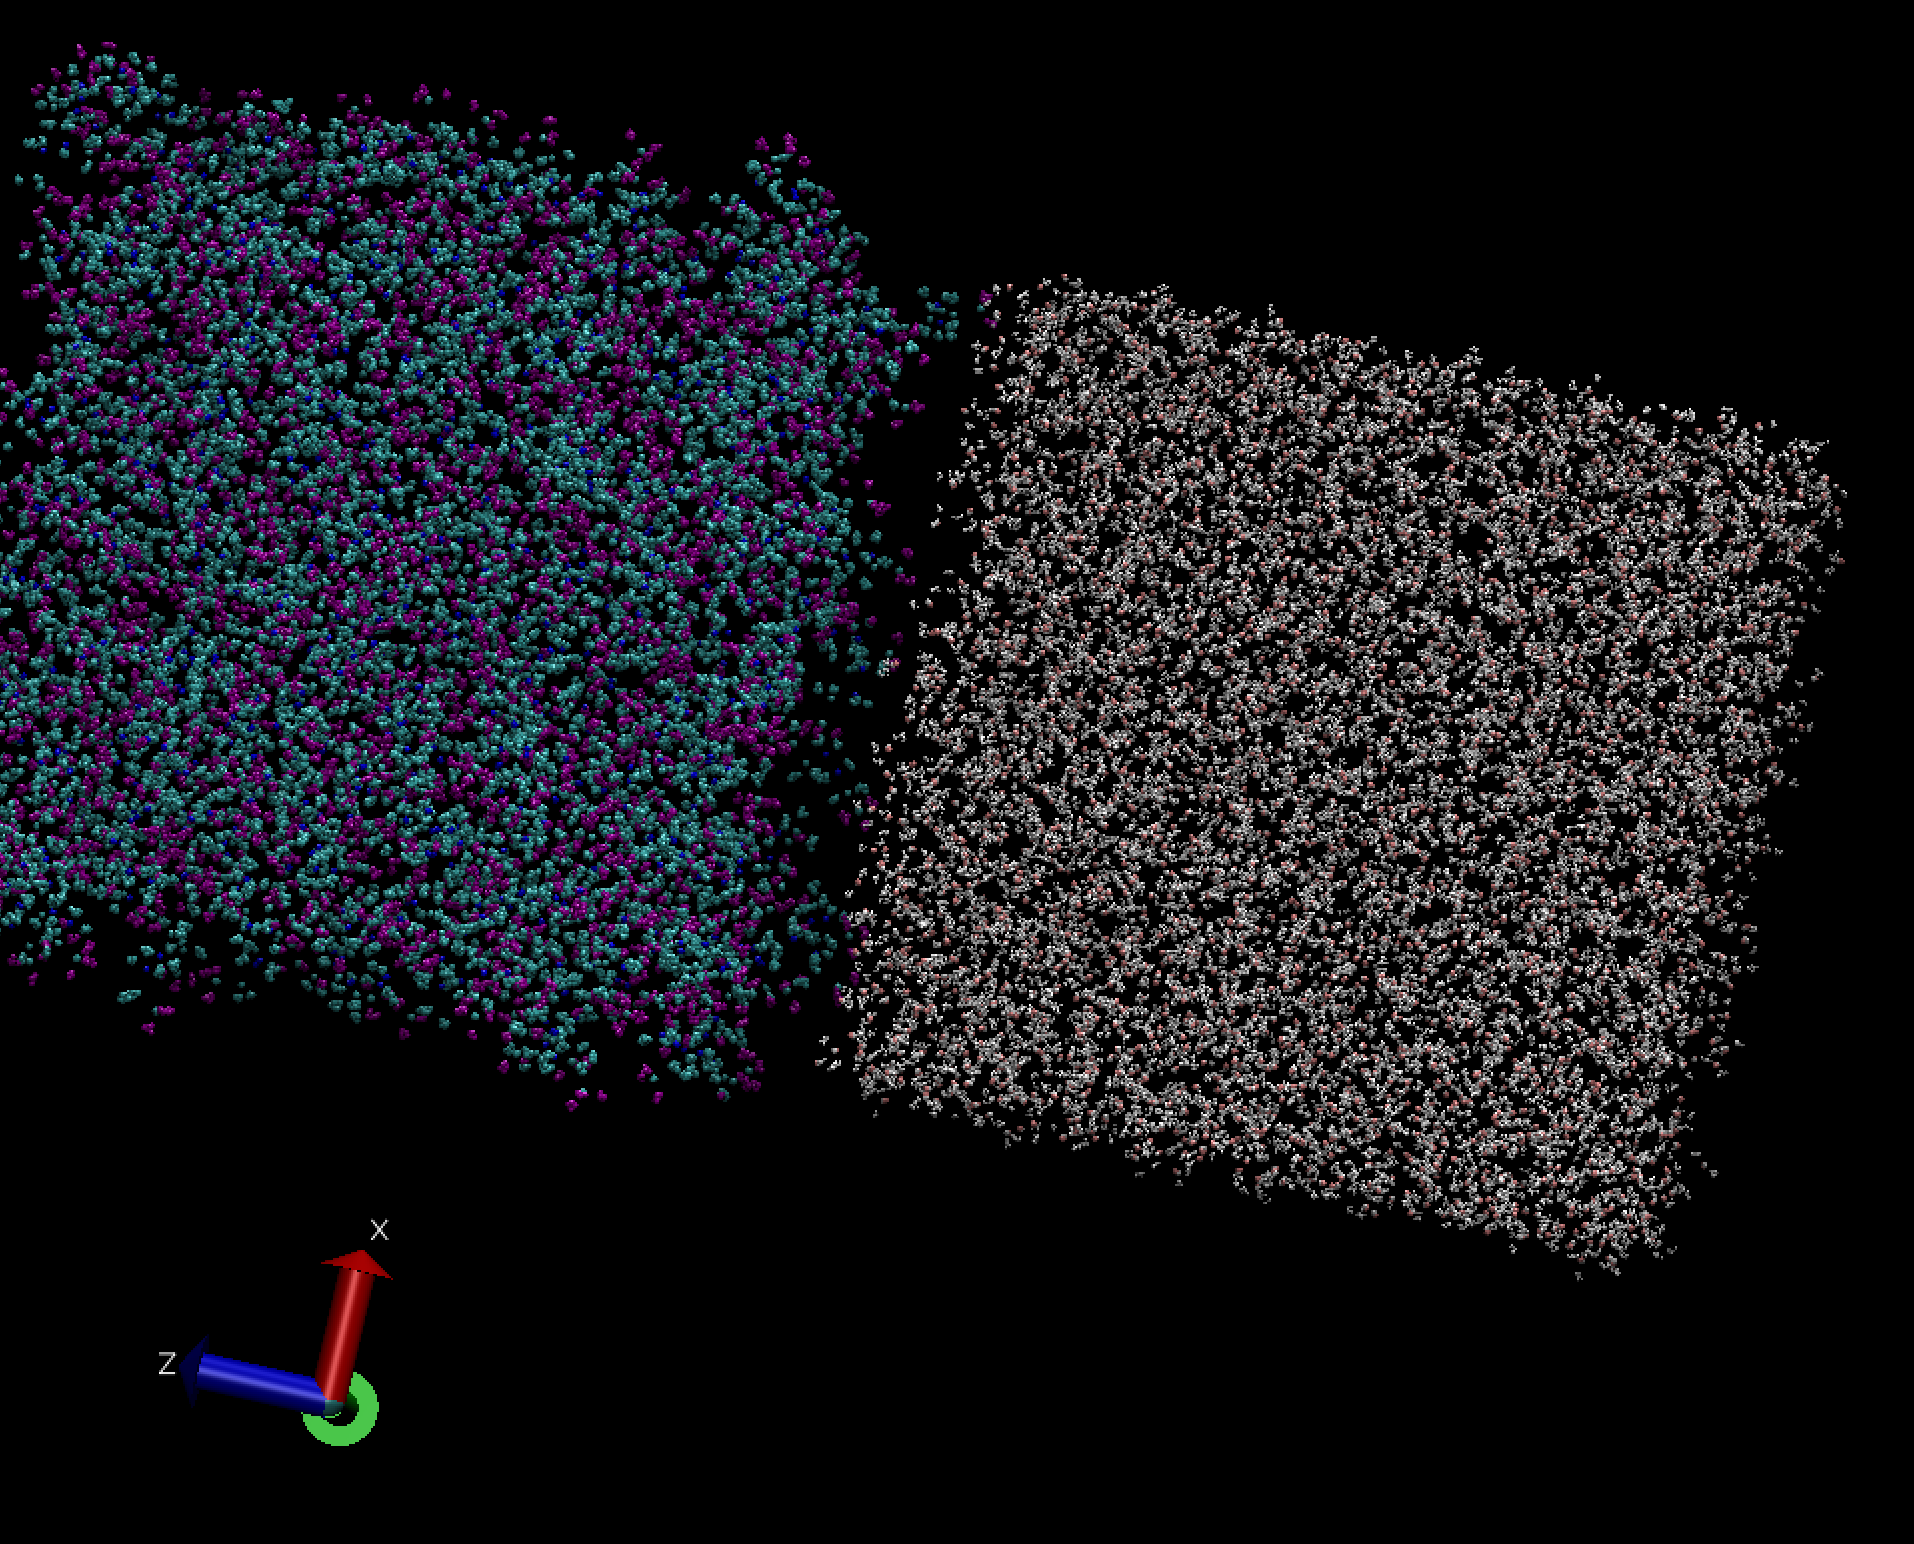
\includegraphics[scale=0.4]{dash_taffi-tip4pF_8beads_0}
\caption{DASH simulation of the TAFFI - q-TIP4P/F interface.  Arithmetic mixing, 4,000,000 time steps.  This is the 0th timestep.}
\end{figure}

\begin{figure}[H]
\centering
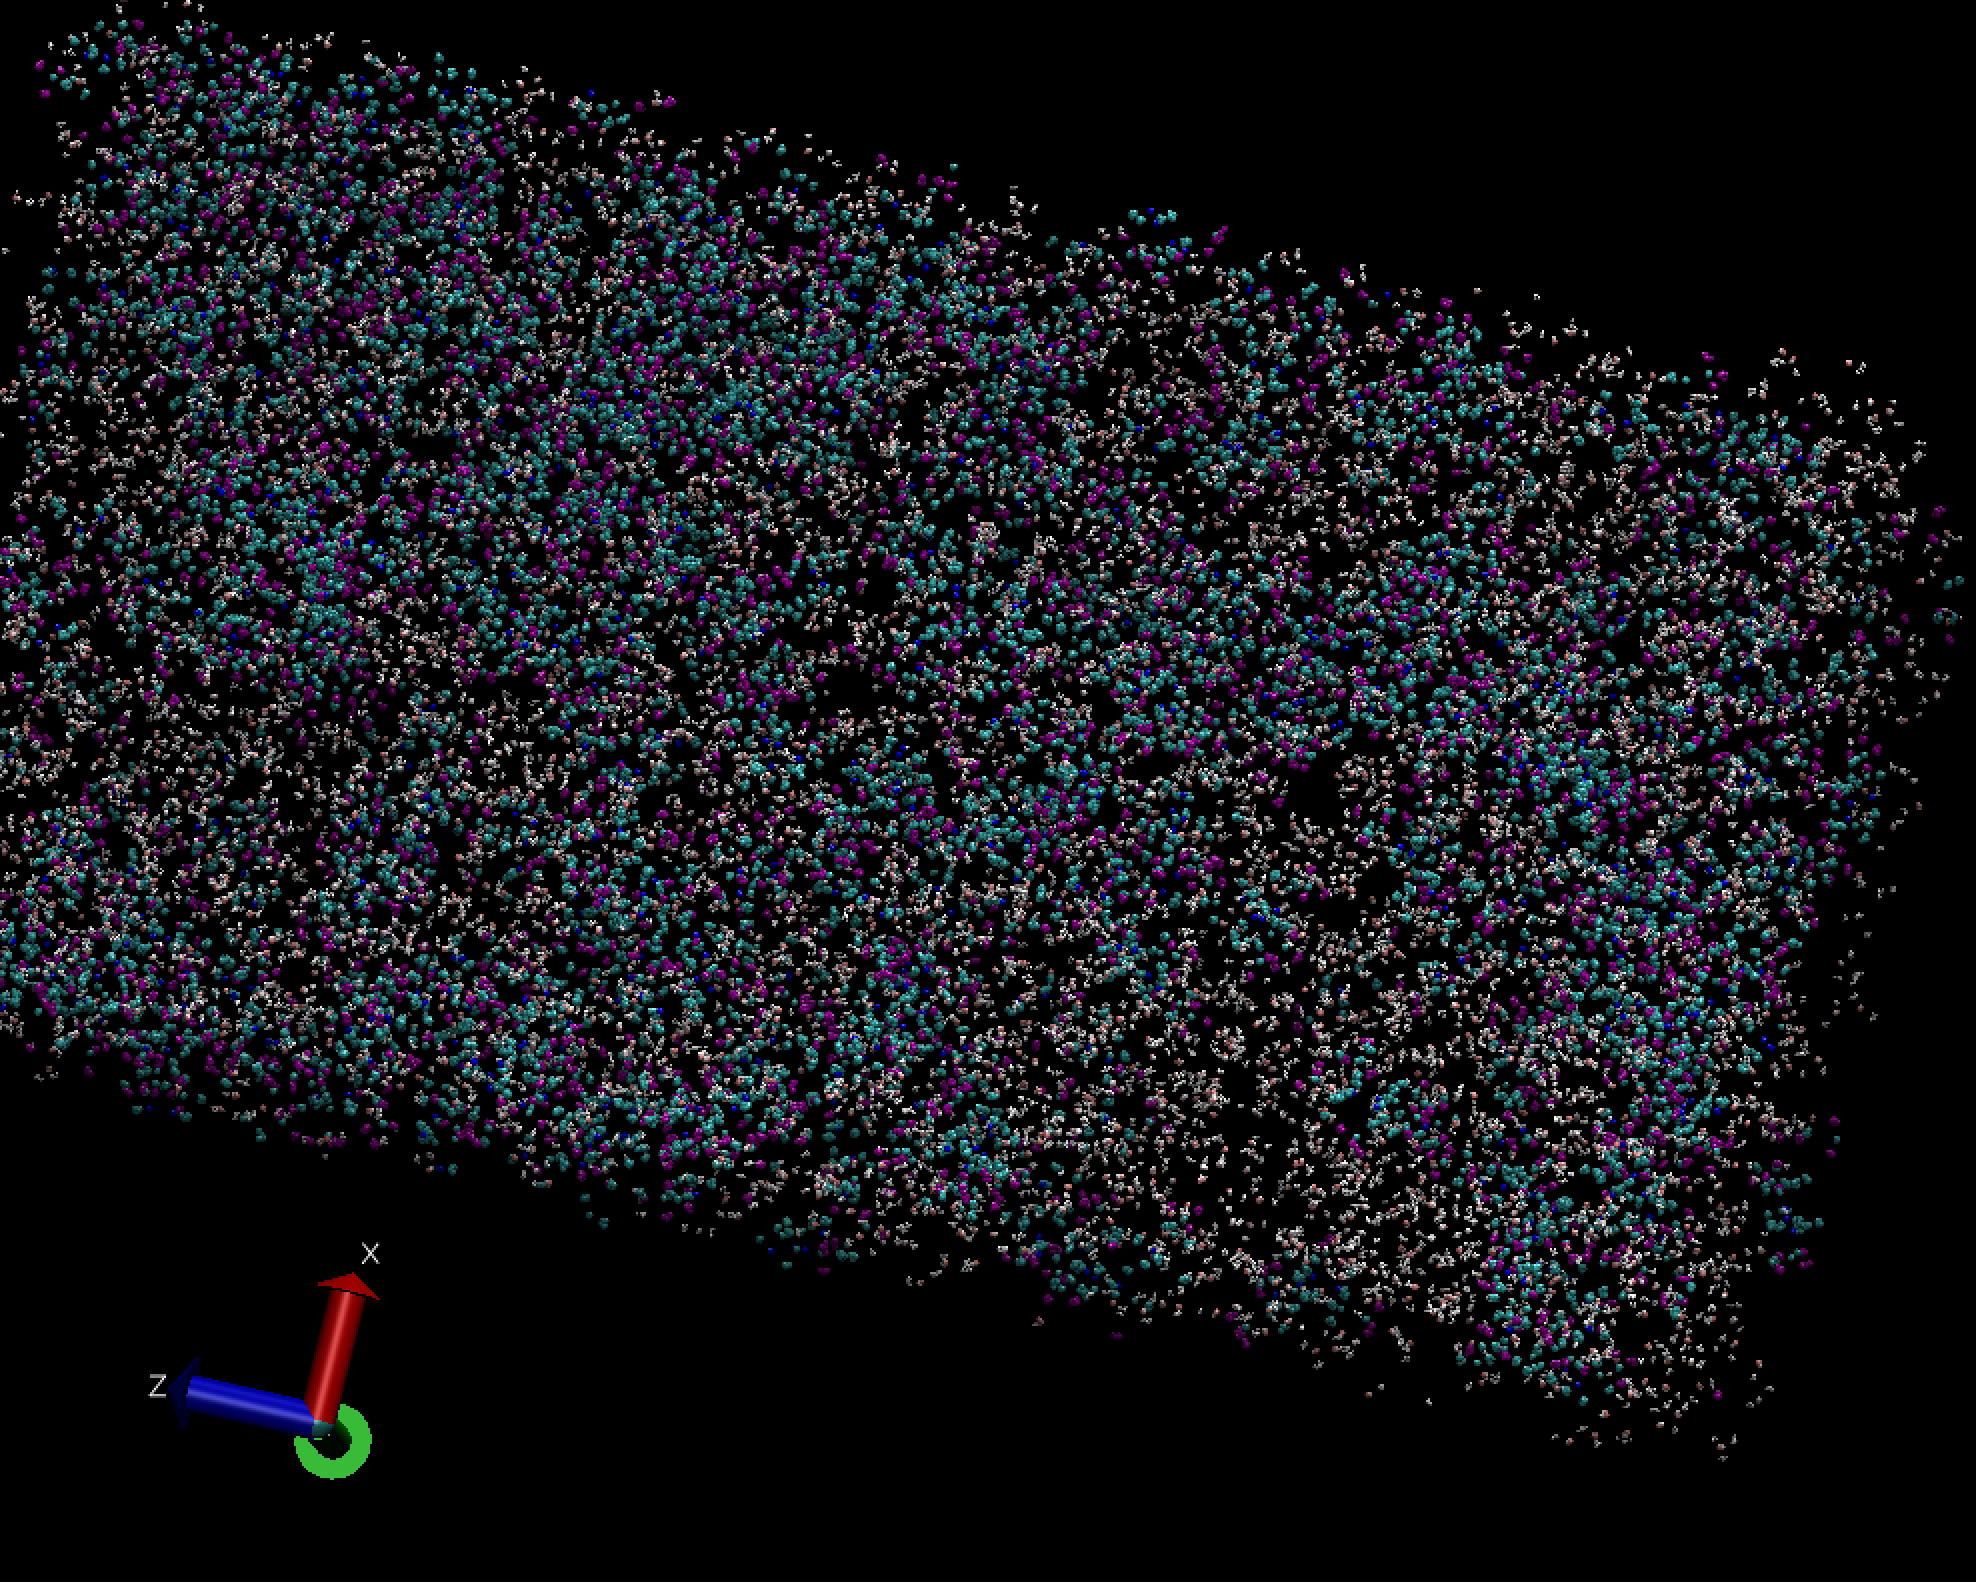
\includegraphics[scale=0.4]{dash_taffi-tip4pF_8beads_3950000}
\caption{DASH simulation of the TAFFI - q-TIP4P/F interface.  Arithmetic mixing, 4,000,000 time steps.  This is the 3,950,000th timestep.}
\end{figure}

\item This is in stark contrast to the amount of mixing that we observed in OPLS + TIP4P/2005 in LAMMPS, which was the appropriate amount of mixing, i.e., very little mixing.  So, there are several possible things going on here.  One is that there is an error in the code.  Another is that there is an error in DASH.  And third is that there is a problem with the interaction parameters between the two force fields.  So, here are the following tests that we are going to run to narrow down the problem:
\subitem Run TAFFI + TIP4P/F in LAMMPS using arithmetic, geometric, and Waldman-Hagler mixing rules and using both TAFFI and OPLS parameters for hexane 
\subitem Run TAFFI + TIP4P/F in DASH using geometric and Waldman-Hagler mixing rules using both TAFFI and OPLS parameters and using 1 bead versus 8 beads
\subitem Run OPLS + TIP4P/F in DASH using geometric mixing rules and using 1 bead versus 8 beads
\subitem Check for any errors in the DASH input scripts
\subitem TAFFI + TIP4P/F in DASH using on bead

\item So, the first step we are going to take is to run TAFFI + q-TIP4P/F in LAMMPS using arithmetic mixing rules.  Let's first take a look at the simulation of TAFFI + TIP4P/2005 and see what that snapshot looks like.  At timestep zero:

\begin{figure}[H]
\centering
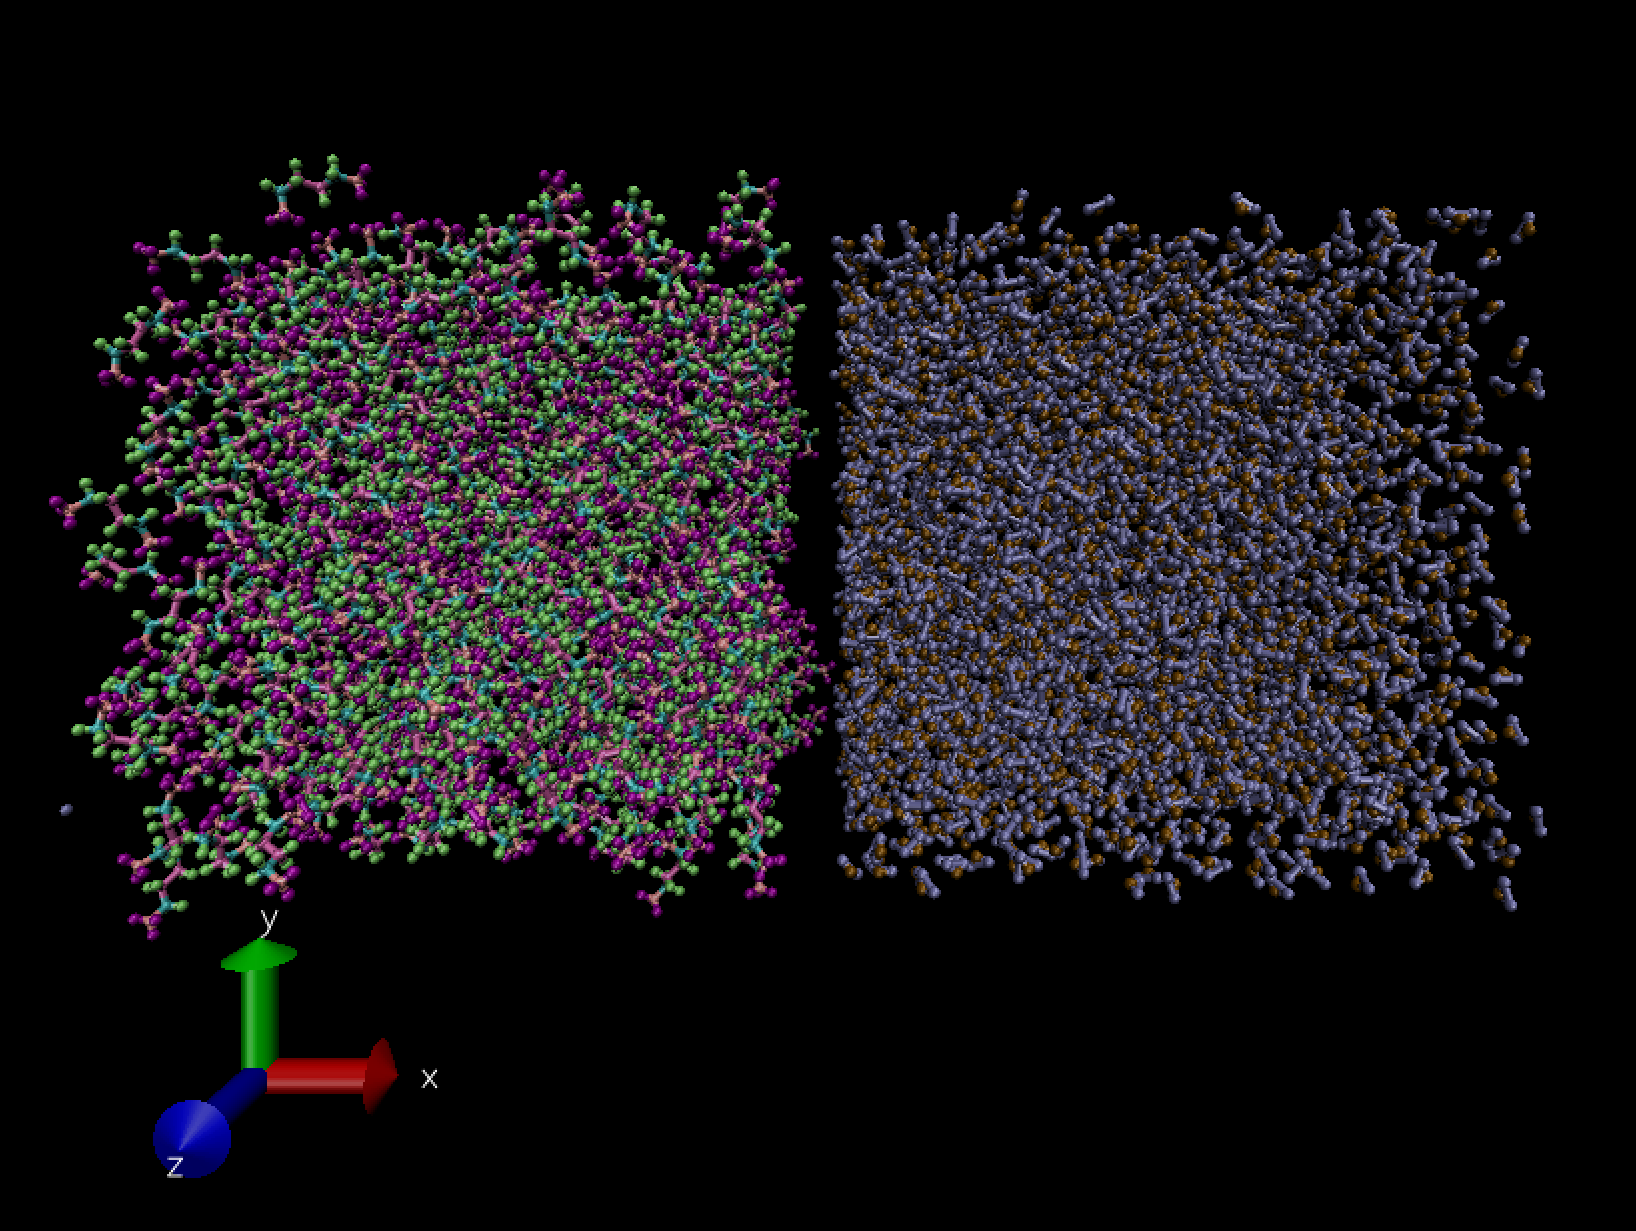
\includegraphics[scale=0.4]{lammps_taffi-tip4p2005_0}
\caption{Lammps simulation of the TAFFI - TIP4P/2005 interface.  Arithmetic mixing, 200,000 time steps.  This is the 0th timestep.}
\end{figure}

After 200,000 time steps:

\begin{figure}[H]
\centering
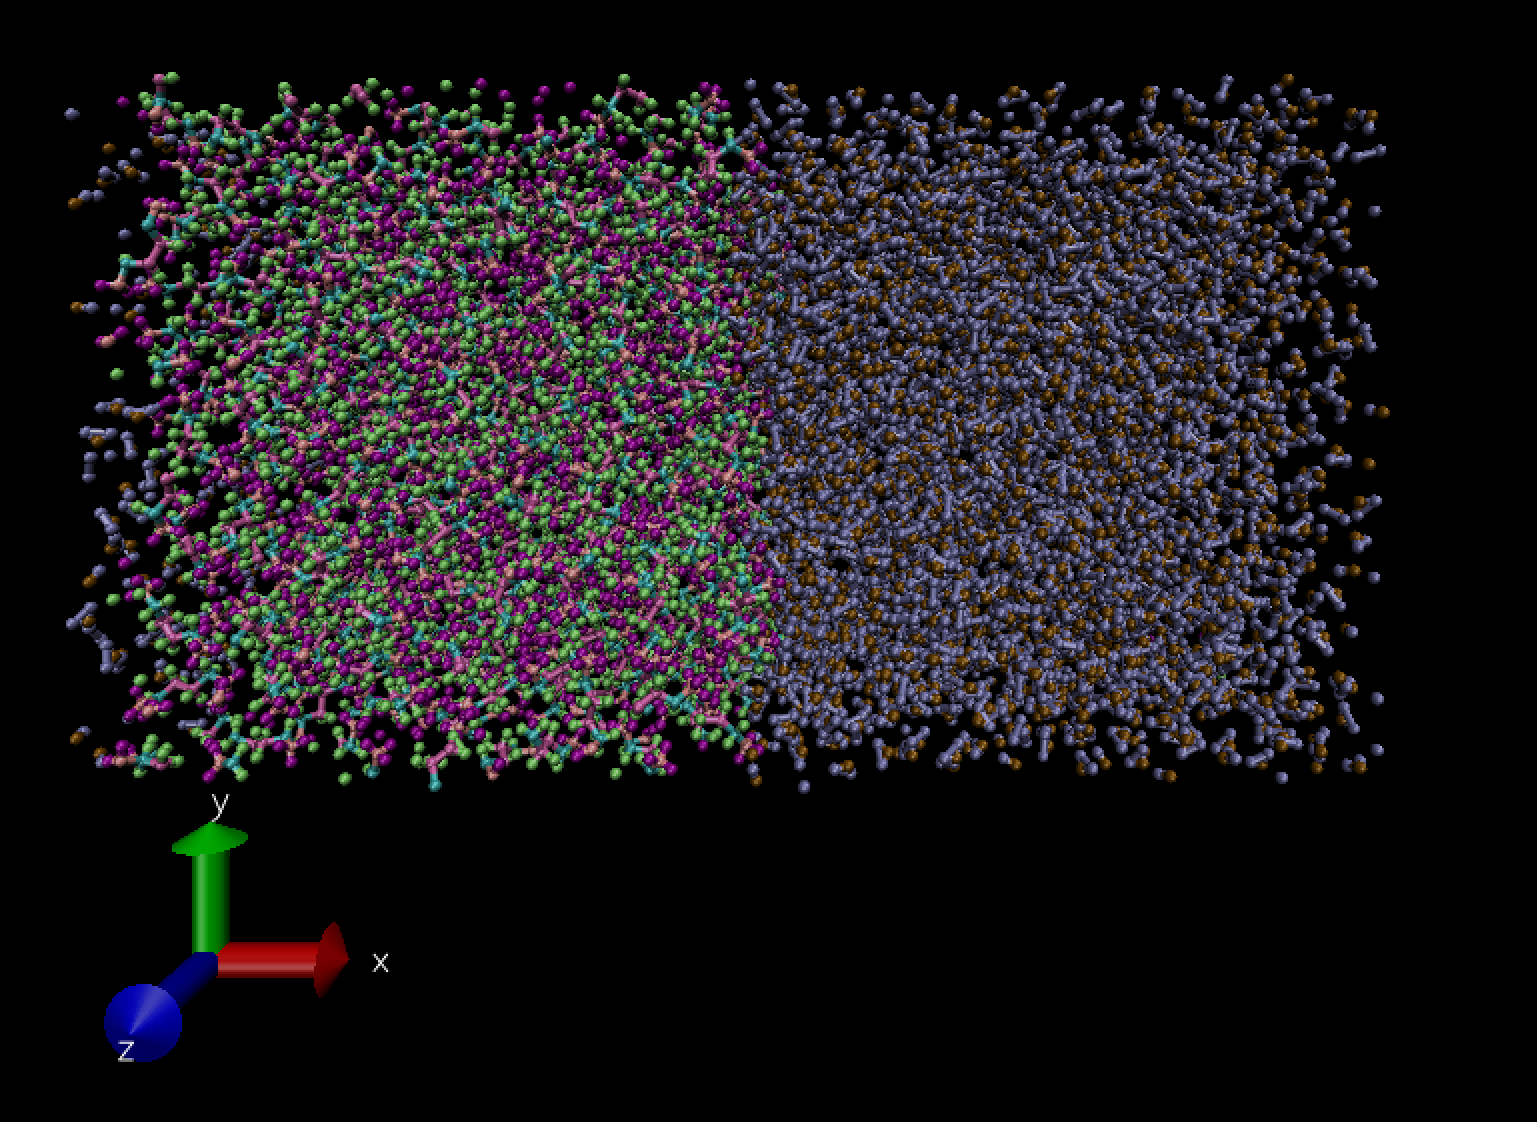
\includegraphics[scale=0.4]{lammps_taffi-tip4p2005_200000}
\caption{Lammps simulation of the TAFFI - TIP4P/2005 interface.  Arithmetic mixing, 200,000 time steps.  This is the 199,000th timestep.}
\end{figure}

For more direct comparison, here is the dash version of TAFFI + TIP4P/F at 200,000 steps:

\begin{figure}[H]
\centering
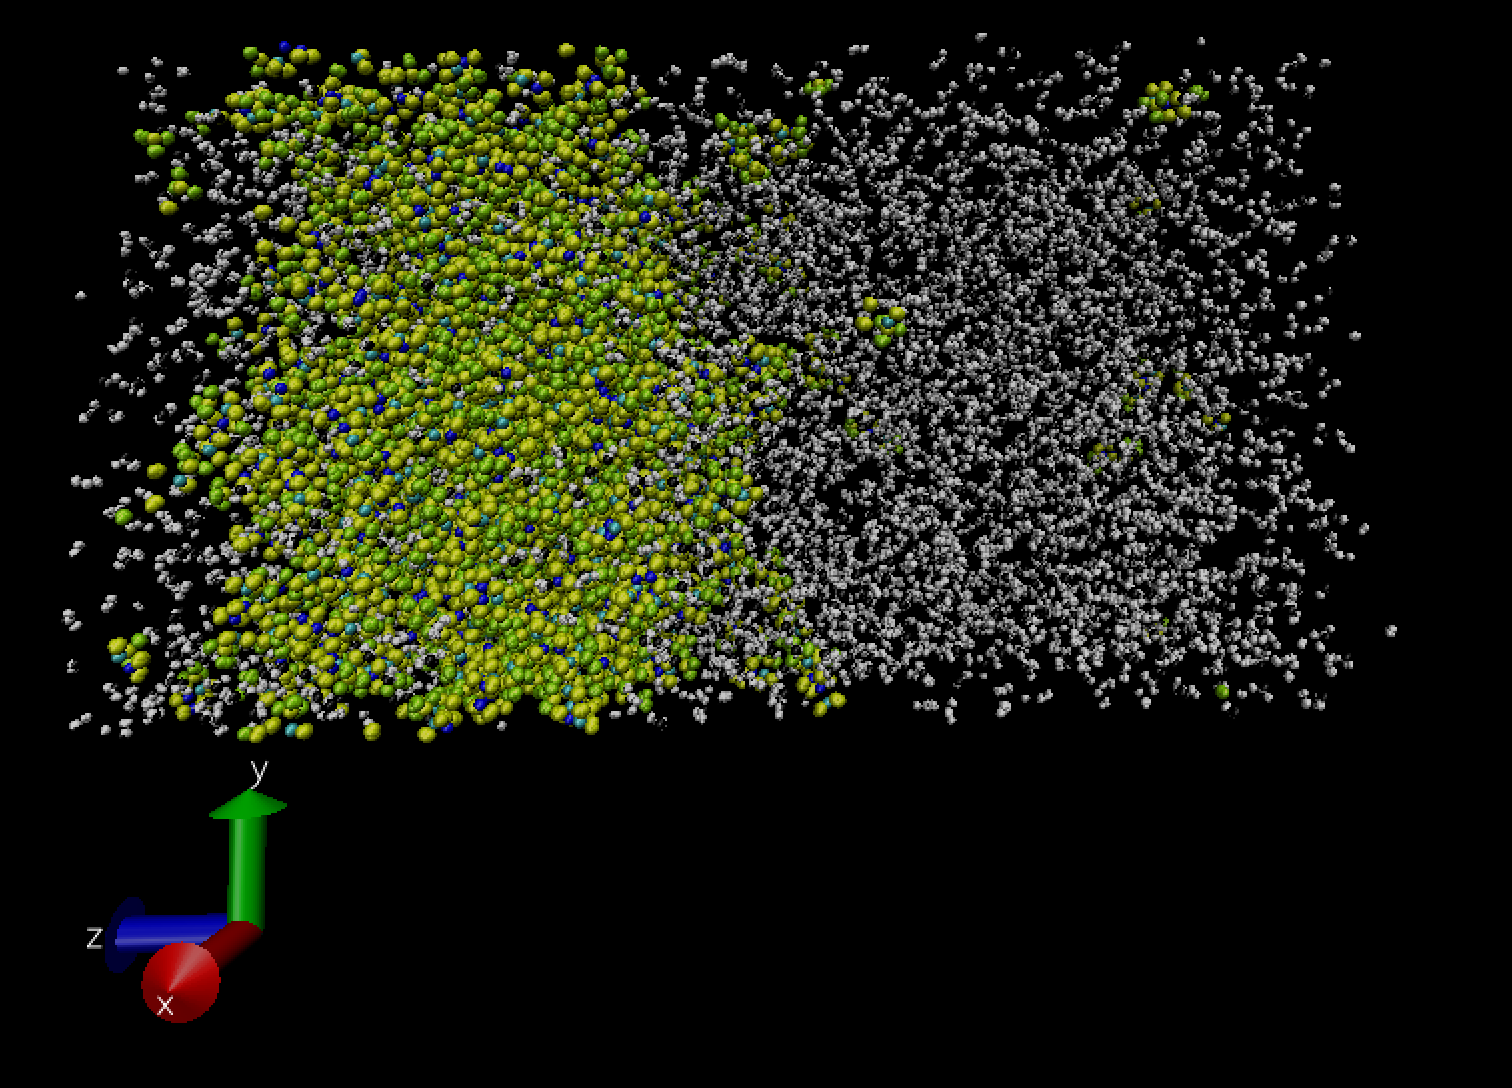
\includegraphics[scale=0.4]{dash_taffi-tip4pF_8beads_200000}
\caption{DASH simulation of the TAFFI - q-TIP4P/F interface.  Arithmetic mixing, 4,000,000 time steps.  This is the 3,950,000th timestep.}
\end{figure}

\item Now, we are going to construct the TIP4P/F in LAMMPS.  The starting point is the TIP4P/2005 classical rigid water model, which we have already implemented.  The next step is to add a quartic expansion of a Morse potential for the OH stretch:
\begin{align}
\begin{split}
V_{OH}(r) = D_r\left[\alpha_r^2(r - r_0)^2 - \alpha_r^3(r - r_0)^3 + \frac{7}{12}\alpha_r^4(r - r_0)^4\right], 
\end{split}
\end{align}
where $D_r = 116.09$, $\alpha_r = 2.287$, and $r_0 = 0.9419$.  

And then we add a simple harmonic potential for the bond angle:

\begin{align}
\begin{split}
V_{HOH}(\theta) = \frac{1}{2}k_\theta(\theta - \theta_0)^2, 
\end{split}
\end{align}
where $k_\theta = 87.85$, and $\theta_0 = 107.4$.


\item In LAMMPS, then, we will try using bond\_style class2 for the quartic expansion of the Morse potential for the OH stretch:

\begin{align}
\begin{split}
E = K_2(r - r_0)^2 + K_3(r - r_0)^3 + K_4(r - r_0)^4,
\end{split}
\end{align}
where $r_0 = r_{eq}$, $K_2 = \alpha_r^2 = 5.23$, $K_3 = -\alpha_r^3 = -11.962$, and $K_4 = \frac{7}{12}\alpha_r^4 = 15.958$.

\item We will use angle\_style harmonic for the simple harmonic potential for the bond angle:

\begin{align}
\begin{split}
E = K(\theta - \theta_0)^2,
\end{split}
\end{align}
where $K = \frac{1}{2}k_\theta$ and $\theta_0 = \theta_{eq} = 107.4$.  

\item Then, we created a data\_water\_flexible.txt file, which is a data file describing a single TIP4P/F water molecule for lammps.  I then created an in.water\_flexible file, a lammps input file to run the flexible water model simulation.  I modified this from the TIP4P/2005 input file by removing the fix shake command and adding the bond\_style class2 command.  I then ran lammps\_molecule\_replicator\_water.py in order to get 3650 flexible water molecules on an initial lattice.  
\item I tried running a lammps simulation using in.water\_flexible, but I am getting the error that the program does not recognize class2.  Turns out that this belongs to the LAMMPS package CLASS2, which might not be compiled for in my folder.  So checking that now.  

\item Compiled LAMMPS with CLASS2, and now able to run the flexible water model.  However, massive forces seem to be appearing as I am getting the error: "Out of range atoms - cannot compute PPPM).  It works better if I make the timestep miniscule, but it still breaks eventually.  Sometimes says missing bonds or atoms.  My guess is that I shouldn't be using the command pair\_style lj/cut/tip4p/long.  So perhaps for next time, what I need to do is just implement the water model irrespective of that particular pair style command, and instead I need to input all of the specifications by hand.  

\item Setting that aside for now, let's turn to DASH again, and try different parameter sets here.  Let's first work just in the classical world, with one bead.  First, let's run TAFFI + TIP4P/F in DASH using TAFFI parameters, geometric mixing, and 1 bead.   
\item This is currently running.
\item Now, let's run TAFFI + TIP4P/F in DASH using TAFFI parameters, arithmetic mixing, and 1 bead.  Just to check/be consistent.  
\item This is also currently running.  

 

\end{enumerate}

\subsection{2/23/2018}
\begin{enumerate}
\item NOTICED AN ERROR: MISSING FACTOR OF 116 IN THE BOND POTENTIAL.  FIX THIS NEXT. 
\end{enumerate}

\subsection{2/27/2018}
\begin{enumerate}
\item Fixed this problem, added the missing factor of 166.09 in the bond potential where it was due.  Saved the resulting new input file.  Currently, running an NPT system of 3650 water molecules in order to generate an initial configuration for the test interface of q-TIP4P/F and TAFFI in LAMMPS.  
\item The TAFFI + TIP4P/F in DASH using TAFFI parameters, arithmetic mixing, and 1 bead finished running.  There is too much mixing going on.  Here is a snapshot at time zero:

\begin{figure}[H]
\centering
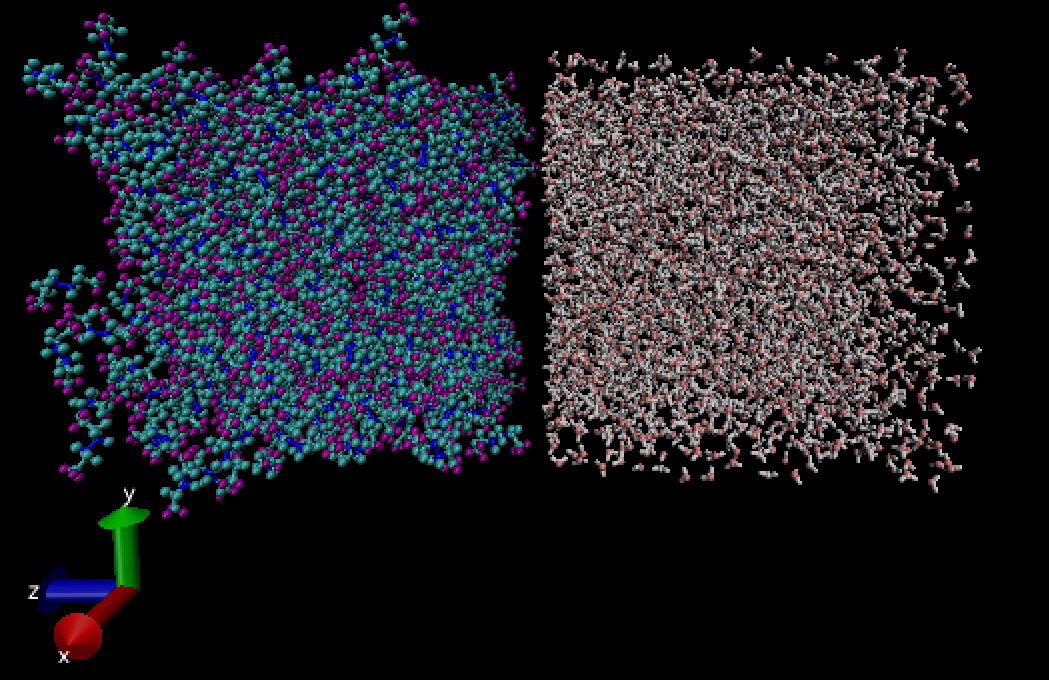
\includegraphics[scale=0.7]{dash_taffi-tip4pF_arithmetic_1bead_0}
\caption{DASH simulation of the TAFFI - q-TIP4P/F interface.  Arithmetic mixing, 4,000,000 time steps, 1 bead.  This is the 0th timestep.}
\end{figure}

\item Here is a snapshot after 4,000,000 timesteps of length 0.5:
\begin{figure}[H]
\centering
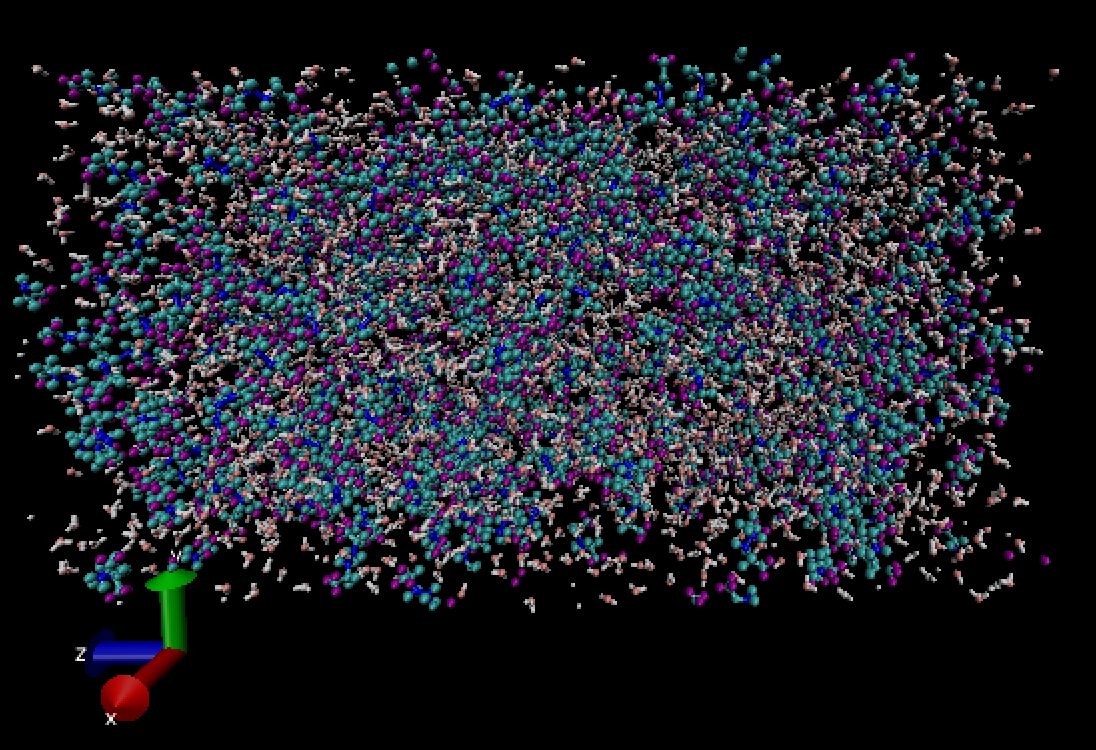
\includegraphics[scale=0.7]{dash_taffi-tip4pF_arithmetic_1bead_3950000}
\caption{DASH simulation of the TAFFI - q-TIP4P/F interface.  Arithmetic mixing, 4,000,000 time steps, 1 bead.  This is the 3950000th timestep.}
\end{figure}

\item The TAFFI + TIP4P/F in DASH using TAFFI parameters, geometric mixing, and 1 bead also finished running.  There is too much mixing.  Here is a snapshot at time zero:

\begin{figure}[H]
\centering
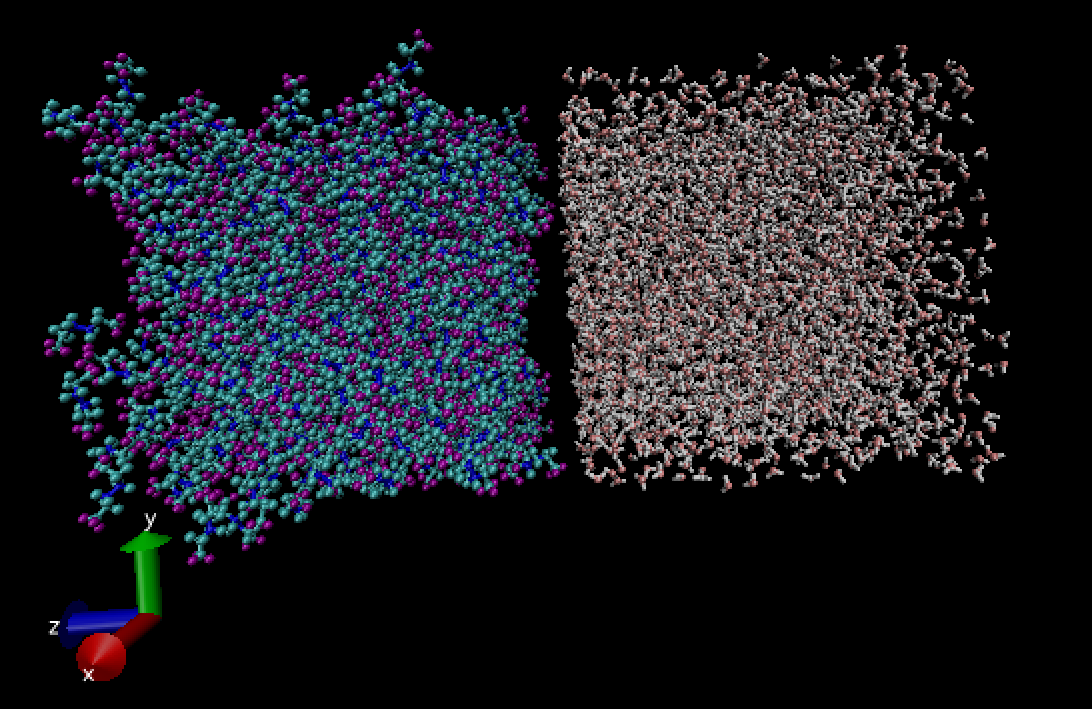
\includegraphics[scale=0.7]{dash_taffi-tip4pF_geometric_1bead_0}
\caption{DASH simulation of the TAFFI - q-TIP4P/F interface.  Geometric mixing, 4,000,000 time steps, 1 bead.  This is the 0th timestep.}
\end{figure}

\item Here is after 4,000,000 timesteps of length 0.5:

\begin{figure}[H]
\centering
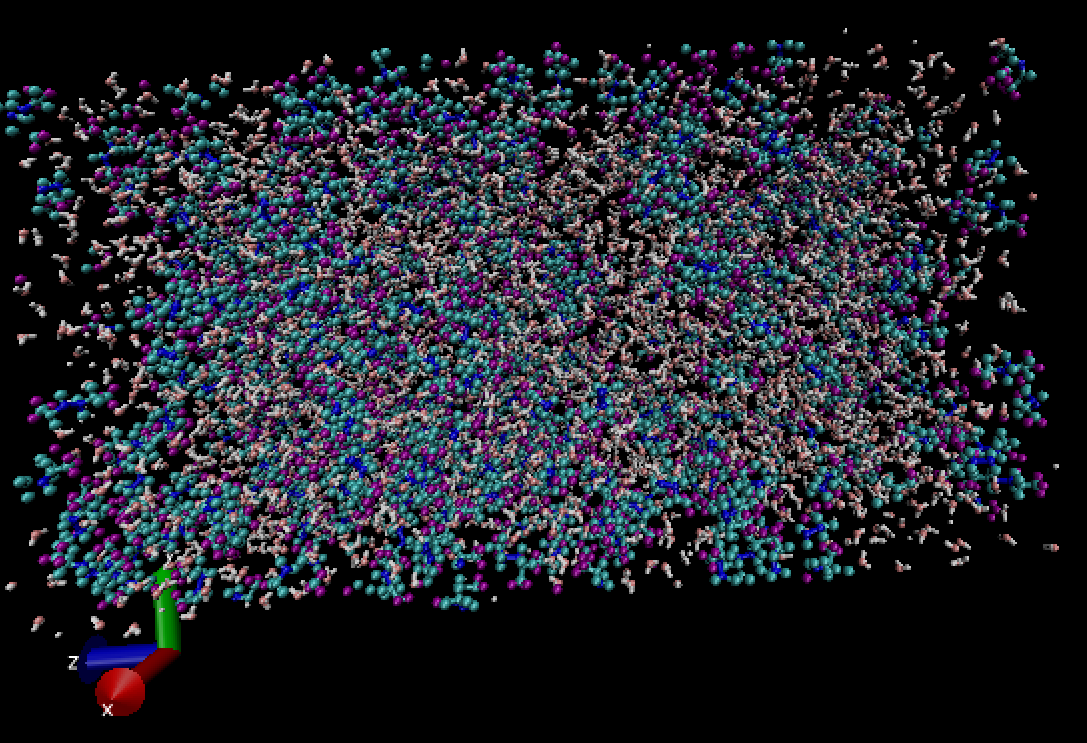
\includegraphics[scale=0.7]{dash_taffi-tip4pF_geometric_1bead_3950000}
\caption{DASH simulation of the TAFFI - q-TIP4P/F interface.  Geometric mixing, 4,000,000 time steps, 1 bead.  This is the 3950000th timestep.}
\end{figure}
  
\end{enumerate}



\subsection{3/5/2018}
\begin{enumerate}
\item Downloaded the trajectory file, dump.water\_flexible.lammpstrj, from the lammps\_work/water folder to check the performance of the TIP4P/F in LAMMPS.  The trajectory looks good.  Moreover, the density of th system reached a final value instantaneous value, at step 200,000, of 0.98752919.  The output file produced, output\_water\_flexible\_preequil.txt, taken after the final 200,000th step in the simulation, also looks reasonable:

 \begin{figure}[H]
\centering
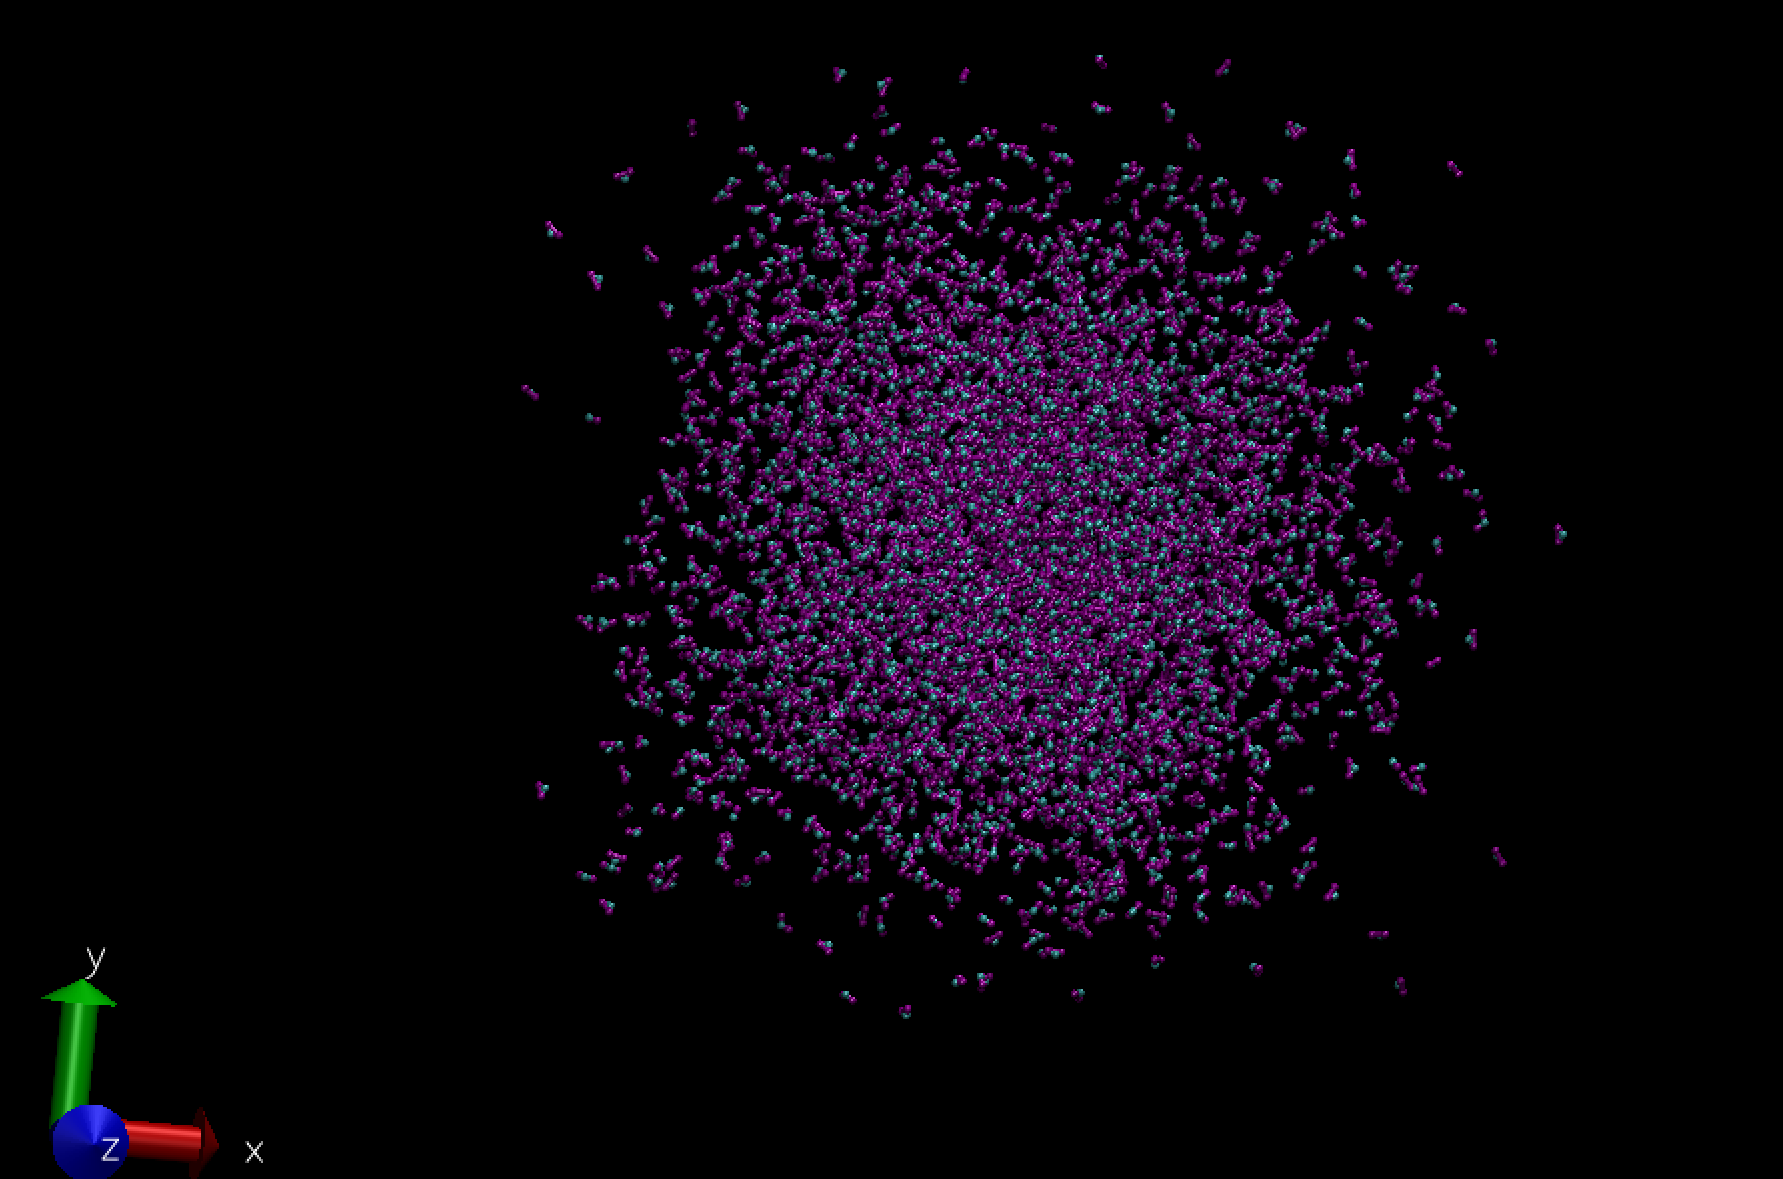
\includegraphics[scale=0.4]{lammps_tip4pF_200000}
\caption{LAMMPS simulation of TIP4P/F water.  Geometric mixing, 200,000 timesteps, this is the final step.}
\end{figure}

\item Now, we will follow steps from before to simulate the TAFFI - q-TIP4P/F interface in LAMMPS.  
\item First, move output\_water\_flexible\_preequil.txt into the interface folder.  Also move the file hexane\_restart\_modified.txt, which is  a preequilibrated slab of TAFFI hexane.  Now, we have two preequilibrated slabs - one with 500 TAFFI hexane molecules, and the other with 3650 TIP4P/F water molecules. 
\item Second, move original molecular data file descriptions of single molecules of TAFFI hexane (i.e. data\_webb\_hexane\_modified.txt) and TIP4P/F water (data\_water\_flexible.txt) to the interface folder.  
\item Run the file lammps\_molecule\_replicator\_tip4pwater\_webbhexane.py in order to produce a mixed system template that can be used as the -dataoriginal input file in the lammps\_restart.py program.  This is what this original file looks like:

\begin{figure}[H]
\centering
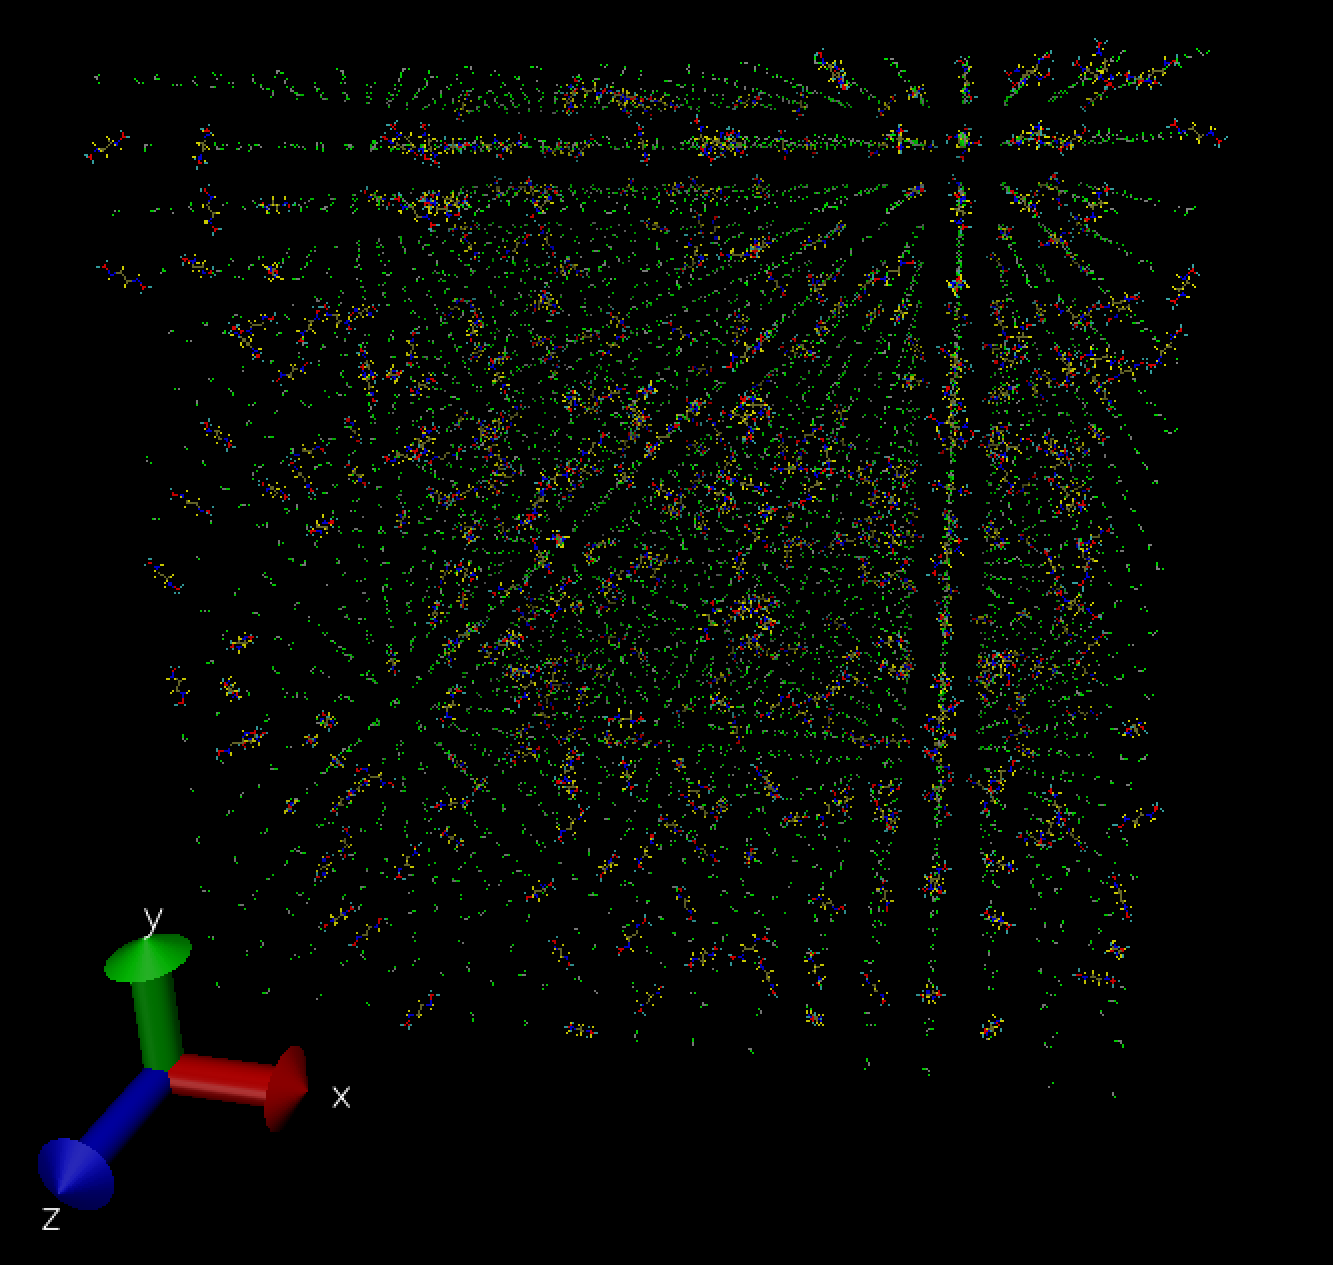
\includegraphics[scale=0.4]{datafileoriginal_taffi_tip4pF}
\caption{Image of datafileoriginal for TAFFI and TIP4P/F.}
\end{figure}

Run the lammps\_restart.py file using -data1=hexane\_restart\_modified.txt, -data2=output\_water\_flexible\_preequil.txt, and -dataoriginal=datafileoriginal\_taffi\_tip4pF.txt.  This produces the initial configuration for the hexane-water TAFFI-TIP4P/F system in LAMMPS:

\begin{figure}[H]
\centering
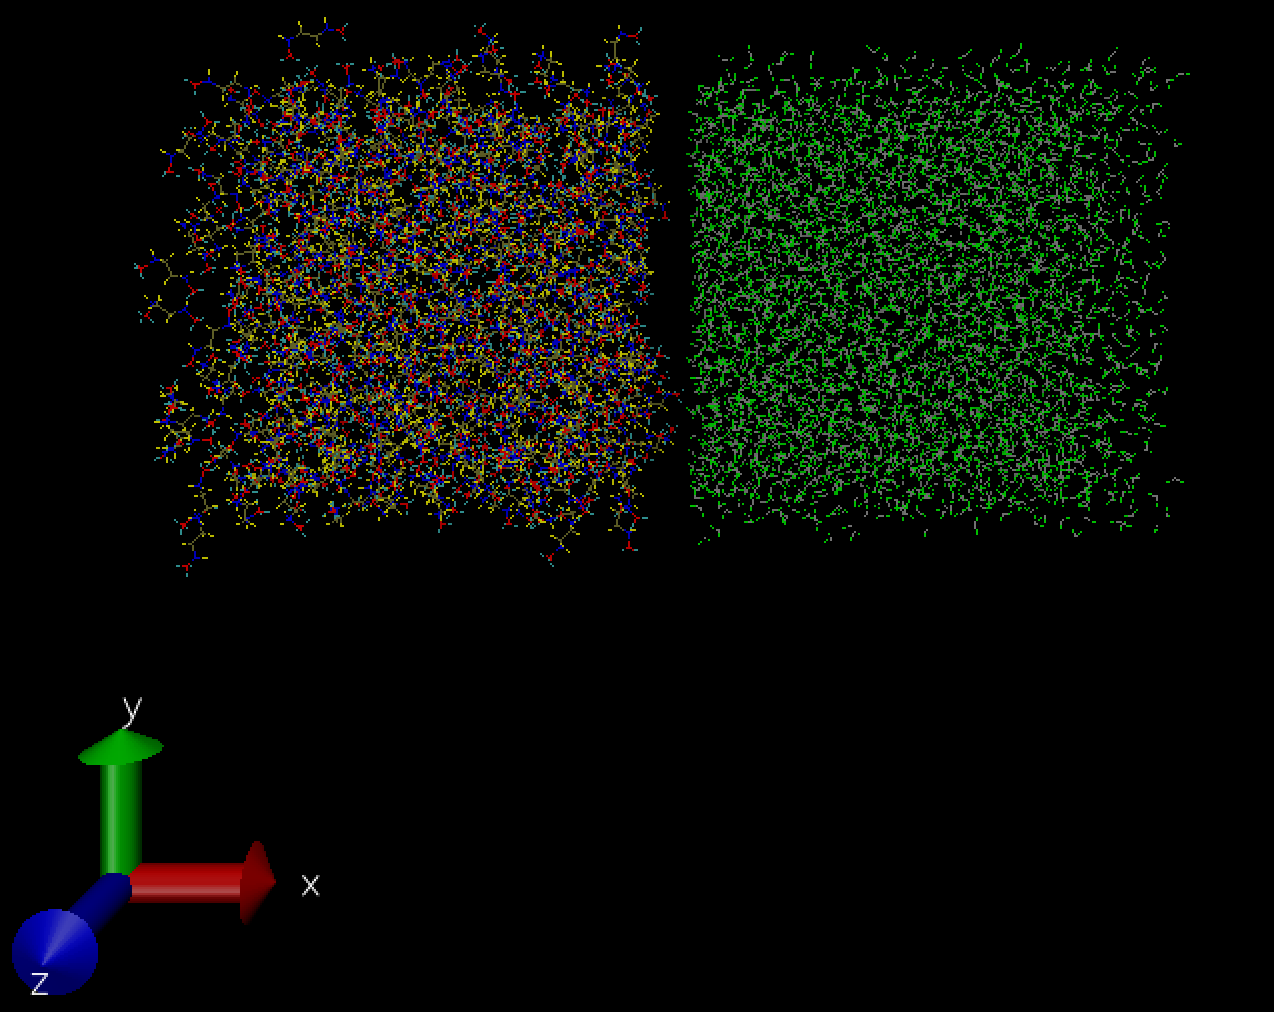
\includegraphics[scale=0.4]{input_restart_taffi_tip4pF}
\caption{Image of input file for TAFFI and TIP4P/F.}
\end{figure}

\item Finally, adjust the input\_restart\_taffi\_tip4pF file to have a Bond Coeffs style that is compatible with bond\_style class2.  

\item HYPOTHESIS: All of my previous LAMMPS	 simulations of the interface were NPT, while in DASH, they were NVT.  Perhaps this is a difference?  I must do all simulations in both to check...

\item I am now running a LAMMPS simulation of the hexane-water interface: 500 TAFFI hexane, 3650 TIP4P/F water, arithmetic mixing, NPT, 200,000 steps of time 1.0.  

\item I am now also running an NVT LAMMPS simulation of the hexane-water interface: 500 TAFFI hexane, 3650 TIP4P/F water, arithmetic mixing, NVT, 200,000 steps of time 1.0.   

\end{enumerate}

\subsection{3/6/2018}
\begin{enumerate}
\item These are snapshots of the NPT simulations:

\begin{figure}[H]
\centering
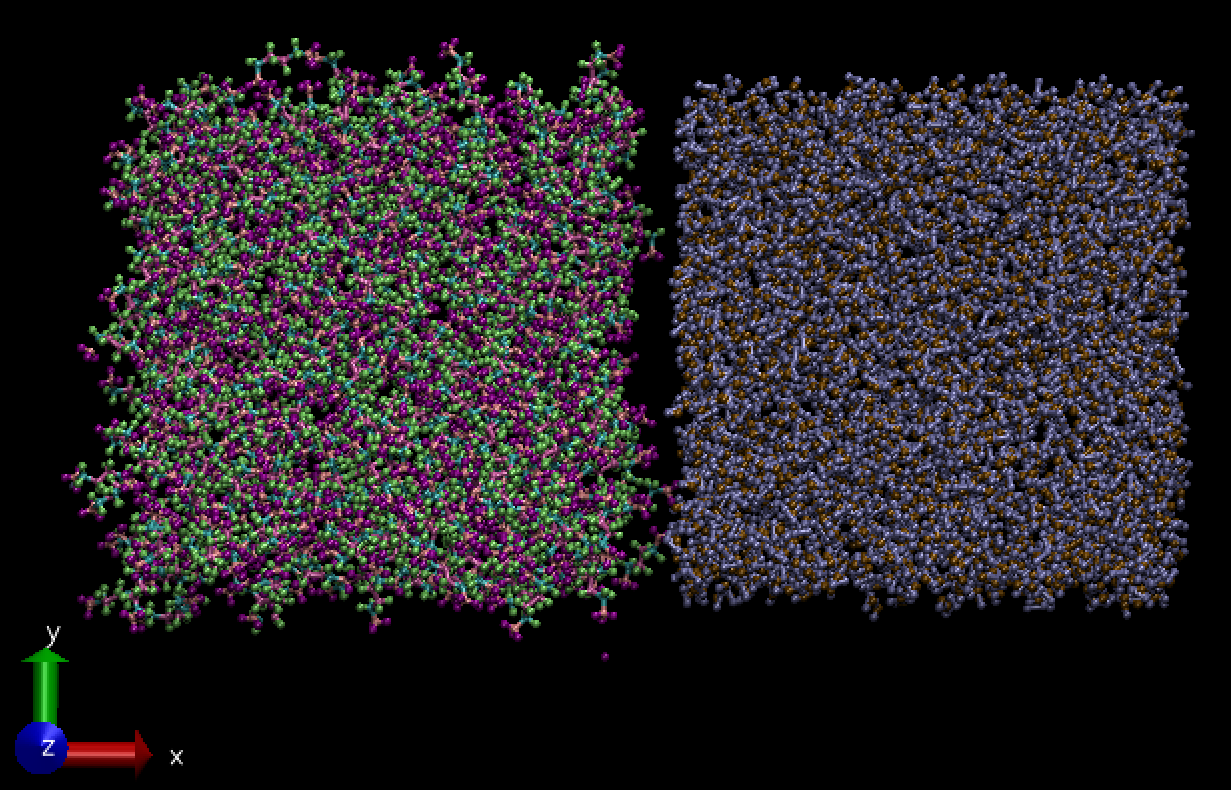
\includegraphics[scale=0.4]{lammps_taffi-tip4pF_0}
\caption{LAMMPS simmulation of 500 TAFFI hexane, 3650 TIP4P/F water, arithmetic mixing, NPT at T = 300 and P = 1, 200,000 timesteps of length 1.0 fs, NPT pre-equilibration of each slab at the same T and P.  Cutoff = 12.0, pppm/tip4p 1e-4, special bonds 0 0 0.  This is the 0th timestep.}
\end{figure}

\begin{figure}[H]
\centering
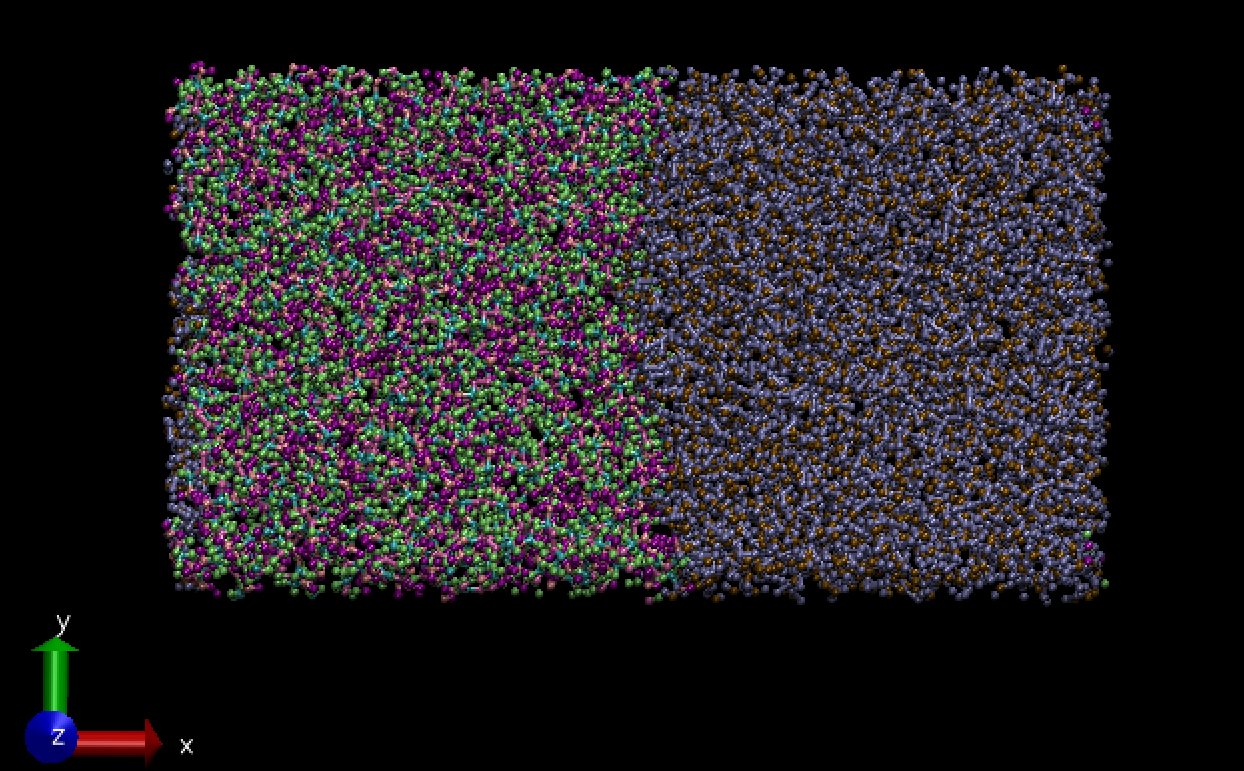
\includegraphics[scale=0.4]{lammps_taffi-tip4pF_200000}
\caption{LAMMPS simmulation of 500 TAFFI hexane, 3650 TIP4P/F water, arithmetic mixing, NPT at T = 300 and P = 1, 200,000 timesteps of length 1.0 fs, NPT pre-equilibration of each slab at the same T and P.  Cutoff = 12.0, pppm/tip4p 1e-4, special bonds 0 0 0.  This is the 200,000th timestep.}
\end{figure}

\item So, the TAFFI-TIP4P/F interface in LAMMPS appears to be stable under NPT conditions.  The final density of this simulation was around 0.854.  

\item These are snapshots of the NVT simulations: 

\begin{figure}[H]
\centering
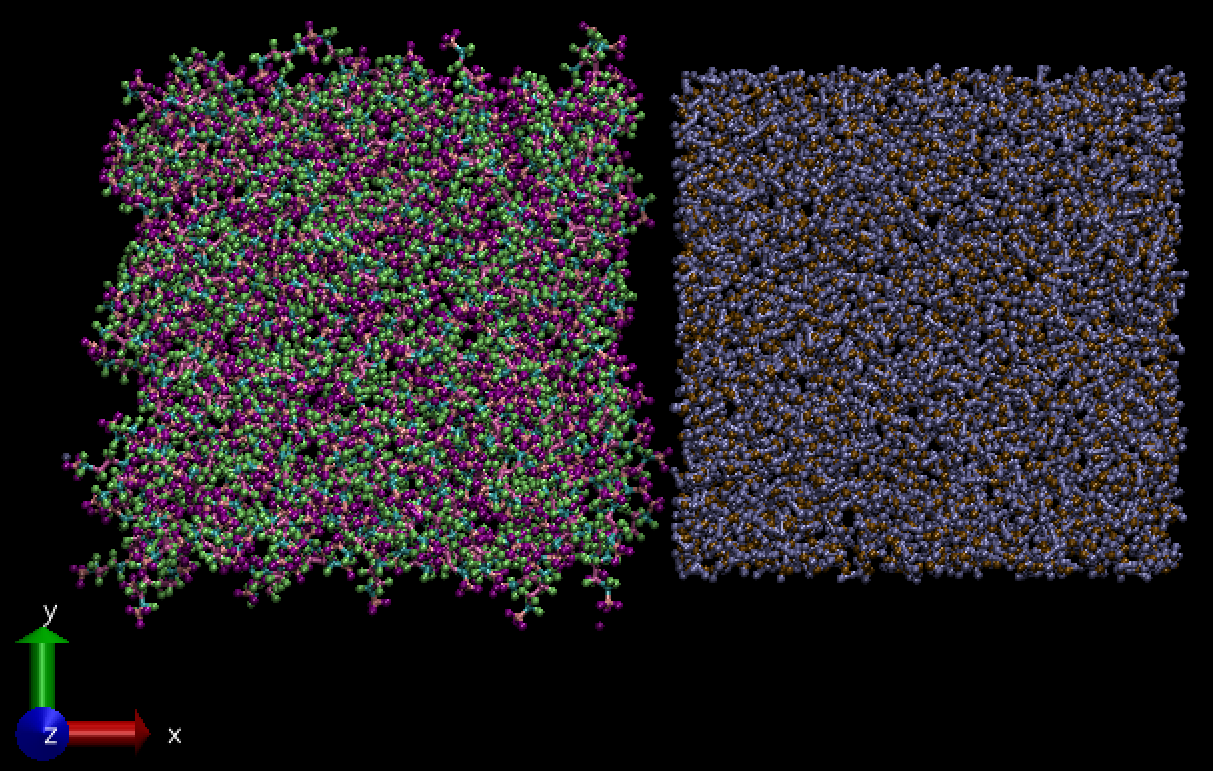
\includegraphics[scale=0.4]{lammps_taffi-tip4pF_NVT_0}
\caption{LAMMPS simmulation of 500 TAFFI hexane, 3650 TIP4P/F water, arithmetic mixing, NVT at T = 300 and V = (4.722, 5.62, 6.26) x (113.25, 64.29, 64.71), 200,000 timesteps of length 1.0 fs, NPT pre-equilibration of each slab at the same T and P = 1.0.  Cutoff = 12.0, pppm/tip4p 1e-4, special bonds 0 0 0.  This is the 0th timestep.}
\end{figure}

\begin{figure}[H]
\centering
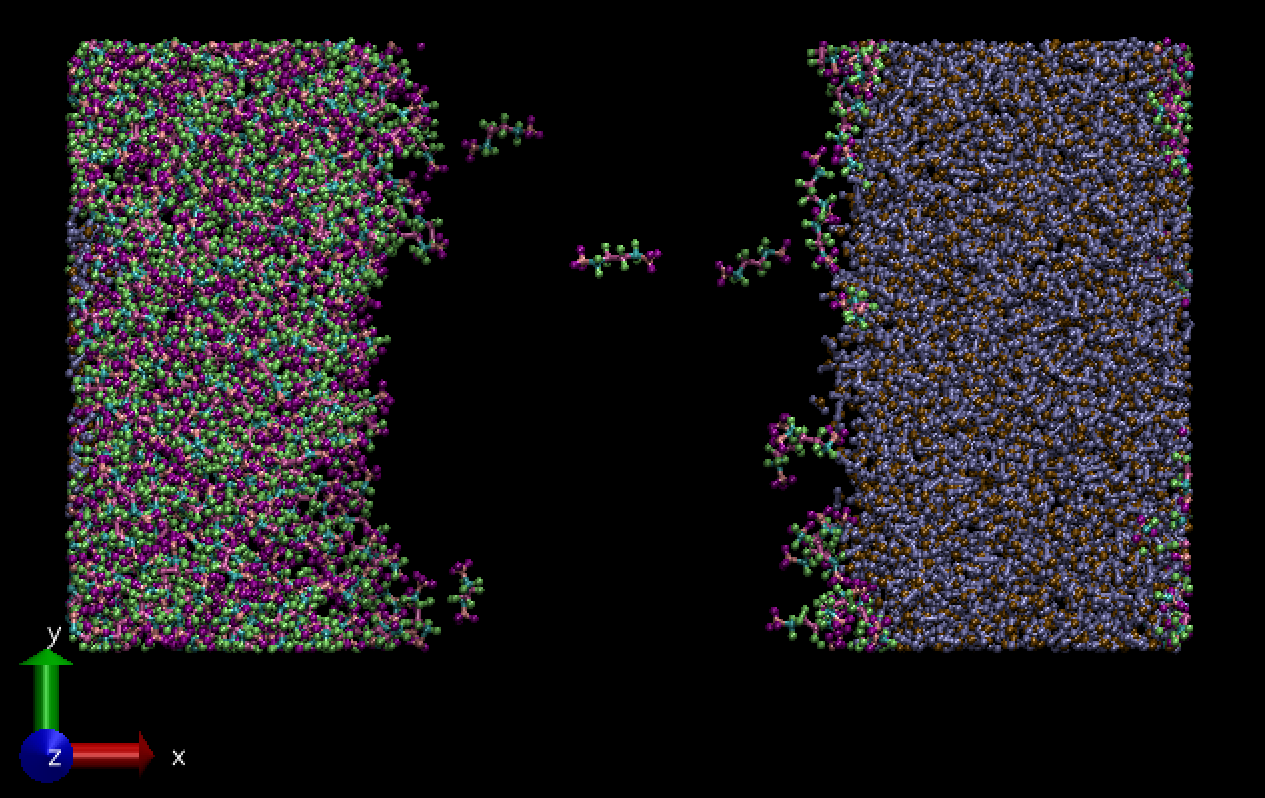
\includegraphics[scale=0.4]{lammps_taffi-tip4pF_NVT_200000}
\caption{LAMMPS simmulation of 500 TAFFI hexane, 3650 TIP4P/F water, arithmetic mixing, NVT at T = 300 and V = (4.722, 5.62, 6.26) x (113.25, 64.29, 64.71), 200,000 timesteps of length 1.0 fs, NPT pre-equilibration of each slab at the same T and P = 1.0.  Cutoff = 12.0, pppm/tip4p 1e-4, special bonds 0 0 0.  This is the 200,000th timestep.}
\end{figure}

\item I have chosen, as usual, the box bounds to be the outermost atoms.  It appears as though this results in a box that is too large for NVT to produce an actual interface in the middle.  However, an interface does exist at the x-boundaries, which appears to be stable.  The final NVT density of the simulation was around 0.4855.    

\item In order to check my new hypothesis, I want to run a classical simulation in DASH of the TAFFI-TIP4P/F interface under NPT conditions.  

These are snapshots of the NPT result:

\begin{figure}[H]
\centering
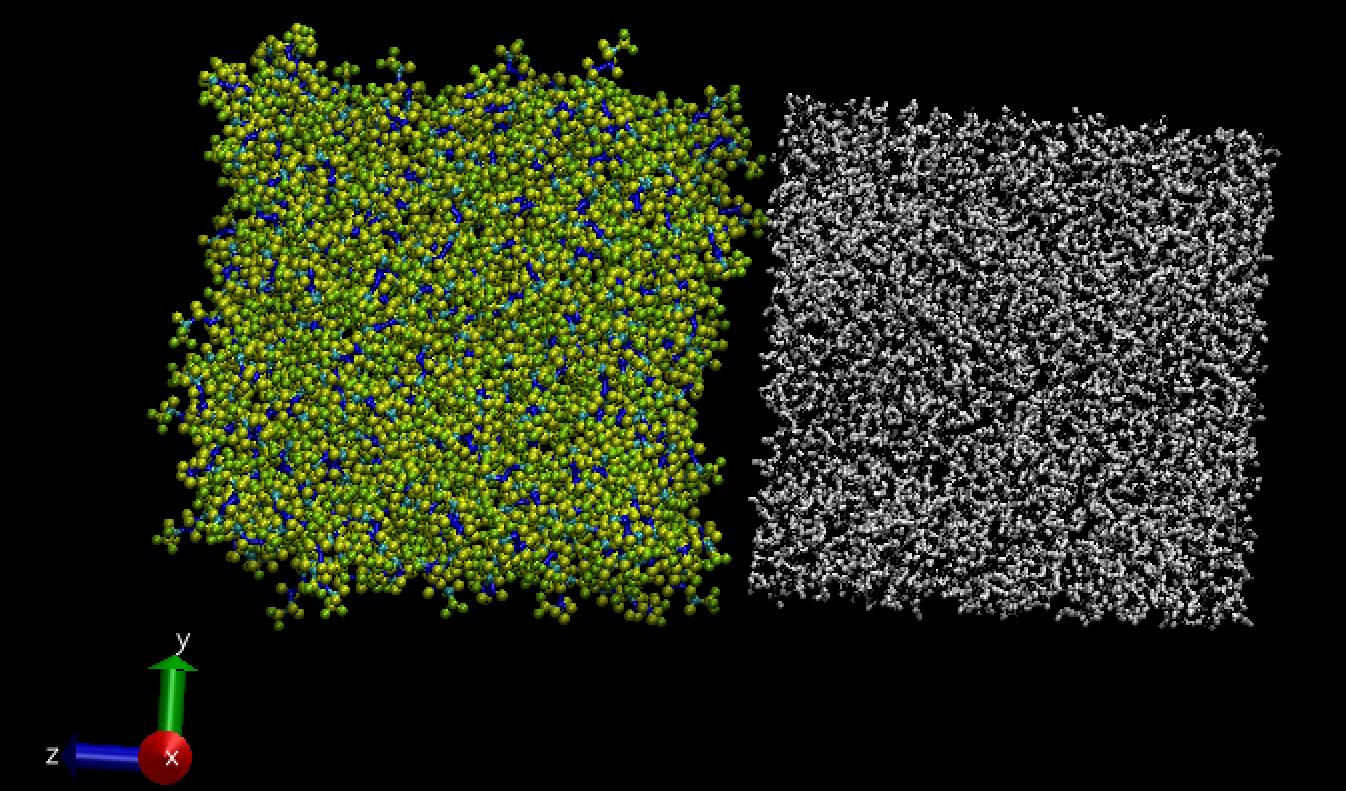
\includegraphics[scale=0.4]{dash_taffi-tip4pF_classical_NPT_0}
\caption{DASH simmulation of 500 TAFFI hexane, 3650 TIP4P/F water, arithmetic mixing, NPT Andersen/Berendsen at T = 300 and P = 1, 200,000 timesteps of length 1.0 fs, NPT pre-equilibration of each slab at 298.15K and same P.  Cutoff = 12.0, Ewald summation.  This is the 0th timestep.}
\end{figure}

\begin{figure}[H]
\centering
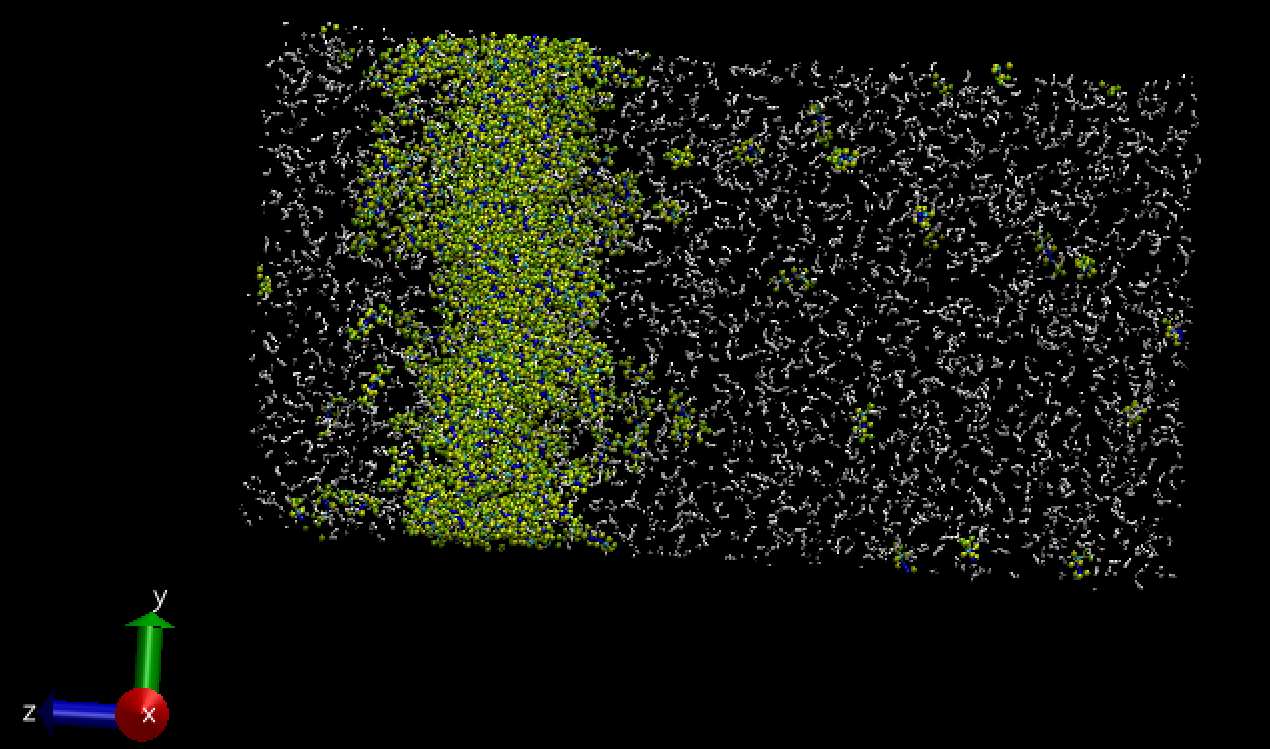
\includegraphics[scale=0.4]{dash_taffi-tip4pF_classical_NPT_200000}
\caption{DASH simmulation of 500 TAFFI hexane, 3650 TIP4P/F water, arithmetic mixing, NPT Andersen/Berendsen at T = 300 and P = 1, 200,000 timesteps of length 1.0 fs, NPT pre-equilibration of each slab at 298.15K and same P.  Cutoff = 12.0, Ewald summation.  This is the 200000th timestep.}
\end{figure}

\item There is a significant difference in the LAMMPS and DASH simulations, suggesting that something is amiss in the DASH program.  

\item I will now check over the interface\_NPT.py script to see if there are any possible sources of error.  We should check: relationship of bulk hexane and water to temperature in DASH, and compared to LAMMPS, as well as specifications of both models, i.e. charge and other parameters.  

\item Went through the interface\_NPT.py file in detail.  Did not find any errors.

\item Now, I am going to run the interface\_NPT.py file with pure water, removing the hexane component, and check the resulting density at various temperatures.  I will then do the same with hexane, removing the water.  Unless I've found the error at this point, I will then do the same calculations in LAMMPS and compare.  

\item It looks like there is an issue with the water.  So, we will start tomorrow with an exploration of what is going on with the pure water restart.  The goal will be to create a water restart within the interface framework that does not have any issues.  

\end{enumerate}

\subsection{3/7/2018}
\begin{enumerate}
\item Looking into pure water simulations in DASH.  
\item First, starting in dash\_work/water folder, running a test version of in.tip4pF.py.  
\item Ran the simulation for 100,000 steps using time length 0.5.  Density approached values aroun 0.98/0.99 by at least before 50,000 steps.  Simulation video looked reasonable.    
\item Ran a restart simulation for 50,000 steps, starting at the previous simulation's 50,000th step.  Density approached 0.985 after the 50,000 steps, which is good.  Video also looks very reasonable.  
\item Tomorrow, I will start with the file in.tip4pF\_restart7.5.py and build from it the hexane-water simulation, checking videos/densities at each step to see where things go wrong!  
\end{enumerate}

\subsection{3/15/2018}
\begin{enumerate}
\item Solved the problem.  The Ewald summation fix was not being activated.  ALL fixes must be activated in DASH.
\item To confirm, currently running: DASH simulation of 500 TAFFI hexane, 4650 TIP4P/F water, arithmetic mixing, NPT Andersen/Berendsen at T = 298.15 K and P = 1.0, 400,000 simulation steps of length 0.5 fs, NPT pre-equilibration of each slab at 298.15 K and 1.0 atm.  Potential cutoff at 12.0, long-range Ewald summation.  Classical simulation, no path integrals.     
\end{enumerate}

\subsection{3/22/2018}
\begin{enumerate}
\item Simulation above finished.  Results are shown below.  The simulation looks clean: 

\begin{figure}[H]
\centering
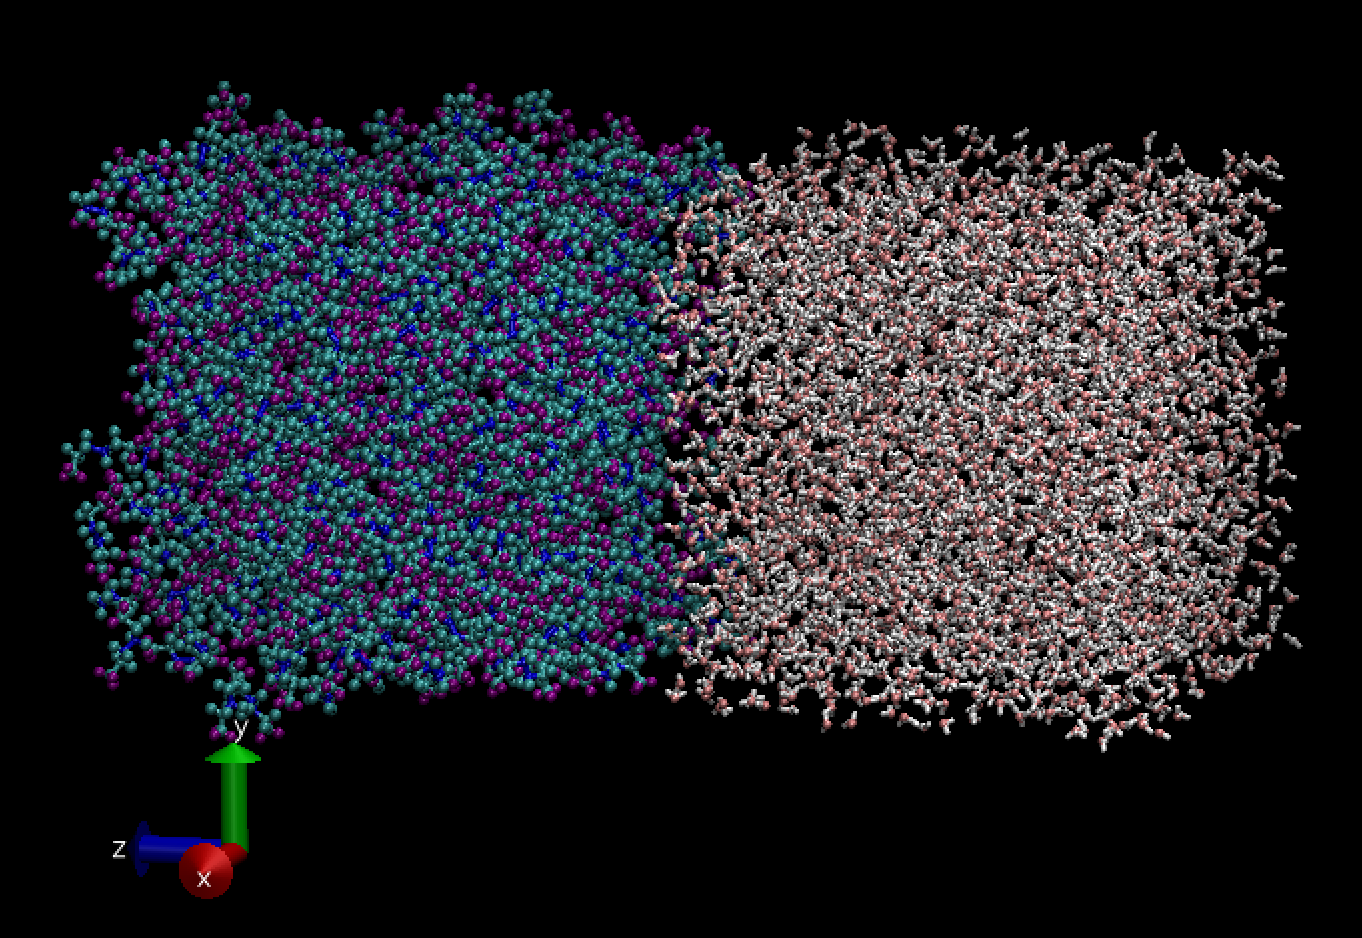
\includegraphics[scale=0.4]{dash_taffi-tip4pF_classical_arithmetic_NPT_0}
\caption{DASH simmulation of 500 TAFFI hexane, 3650 TIP4P/F water, arithmetic mixing, NPT Andersen/Berendsen at T = 298.15K and P = 1 atm, 240,000 timesteps of length 0.5 fs, NPT pre-equilibration of each slab at 298.15K and same P.  Cutoff = 12.0, Ewald summation.  Classical simulation, no path integrals.  This is the 0th timestep.}
\end{figure}

\begin{figure}[H]
\centering
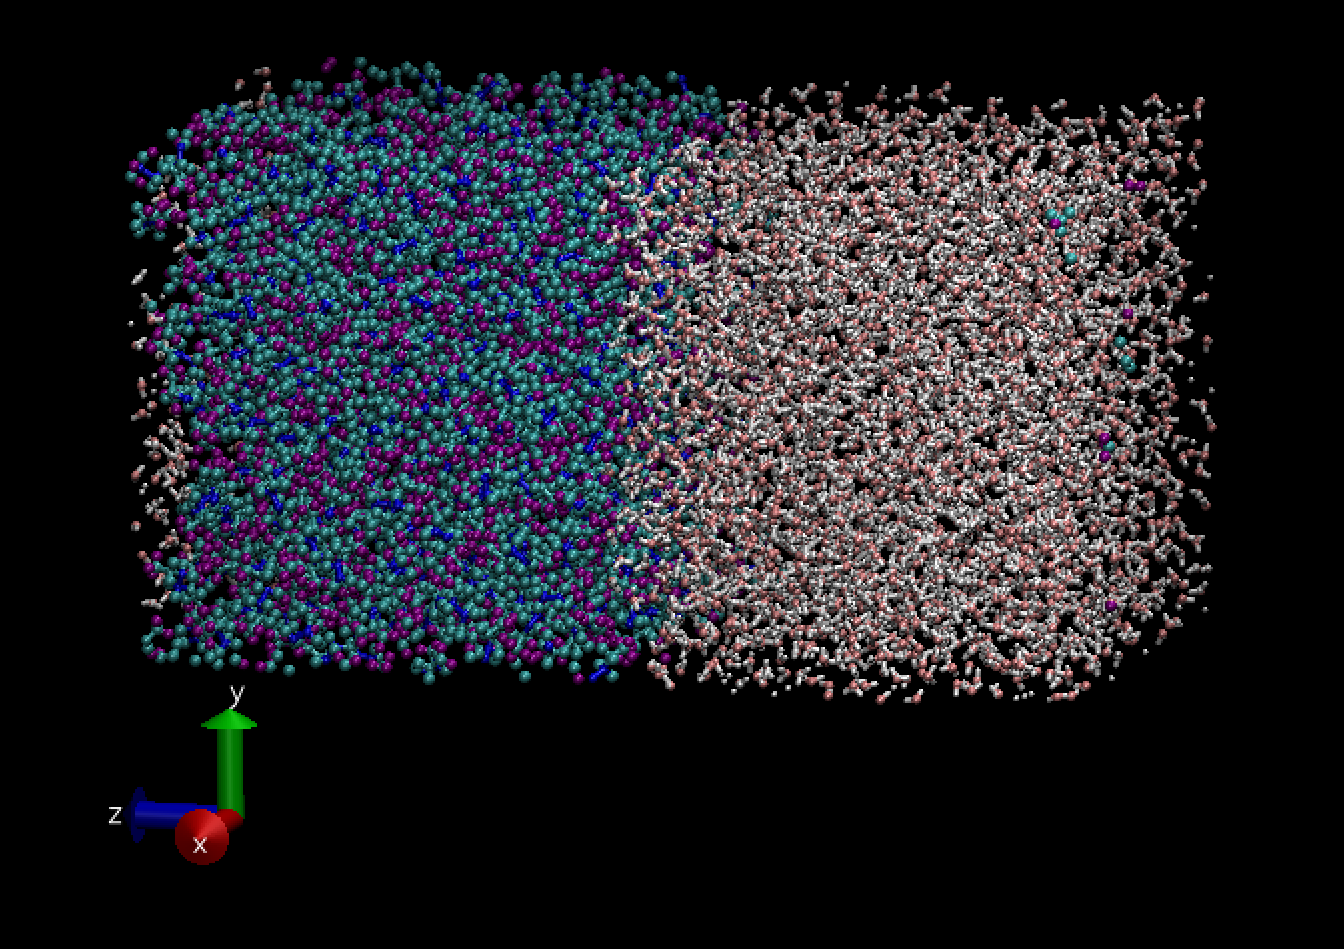
\includegraphics[scale=0.4]{dash_taffi-tip4pF_classical_arithmetic_NPT_400000}
\caption{DASH simmulation of 500 TAFFI hexane, 3650 TIP4P/F water, arithmetic mixing, NPT Andersen/Berendsen at T = 298.15K and P = 1 atm, 240,000 timesteps of length 0.5 fs, NPT pre-equilibration of each slab at 298.15K and same P.  Cutoff = 12.0, Ewald summation.  Classical simulation, no path integrals.  This is the 400,000th timestep.}
\end{figure}

\end{enumerate}

\subsection{3/26/2018}
\begin{enumerate}
\item Added a python operation to interface.py that collects densities information.  Ran a test: DASH simulation of 500 TAFFI hexane, 3650 TIP4P/F water, arithmetic mixing, NPT Andersen/Berendsen at T = 298.15K and P = 1.0 atm, 400,000 timesteps of length 0.5 fs, NPT pre-equilibration of each slab at 298.15K and same P.  Cutoff = 12.0, Ewald summation.  Classical simulation, no path integrals.  
\item After 400,000 steps, the density profiles converge to the following: 0.9858, 1.0191, 0.9989, 1.0086, 0.7922, 0.0233, 0, 0, 0, 0.1867, which are values for the z-axis cut into 10 slices, starting from the water end at negative z and moving in the positive z direction.  Took about 200,000 steps to converge to this density profile.  Next time, we will do a more fine-grained one, check how they are actually computed in papers, then run this and plot the result and compute the 90-10 width! 
\end{enumerate}T

\subsection{3/27/2018}
\begin{enumerate}
\item From Patel, section C.1.: "The density profiles are computed from the average molecular density in 0.5 Angstrom slabs parallel to the liquid-vapor interface.  The average profile is block averaged over 200 ps trajectory blocks from a total run of 3 ns."  
\item We will begin first with "simple" block averaging.  We will do 200,000 fs of system equilibration and then 3,000,000 fs of system run.  In terms of the program, what we need to do is just write the densities in 0.5 Angstroms slabs parallel to the z-axis.  FOR THE TIME BEING, I'm going to do this in NVT, simply because constant volume will lend itself better to a consistent way of computing density profiles.  However, we will do the initial equilibration in NPT.  
\item Wrote a temporary program, interface\_densities.py, that records the density profiles using 200 bins. It has NPT equilibration for 400,000 steps and then computes density profiles every 1000 steps for 200,000 steps in NVT conditions.  This is running now.
\item I also wrote density\_profile\_analysis.py which will plot the density profile. 
\item So, the next step will be to check this result in the density profile analysis tool and then develop the full machinery for analyzing the water density profile, followed by other profiles etc. more rigorously.  
\end{enumerate}

\subsection{3/29/2018}

\begin{enumerate}
\item Need to write a program that can take the hexane\_restart.txt file and the output\_interface.xml file as inputs and restart a simulation of the interface.  This way, we can avoid the time-consuming problem of doing pre-equilibration.  Pre-equilibration can be done as just one run.  This process shouldn't be too hard.  
\item Performed the following simulation: DASH simulation of 500 TAFFI hexane, 3650 TIP4P/F water, arithmetic mixing, NPT Andersen/Berendsen at T = 298.15 K and P = 1.0 atm, 300,000 timesteps of length 0.5 fs equilibration followed by 1000 production steps of length 0.5 fs, NPT pre-equilibration of each slab at 298.15 K and same P.  Cutoff = 12.0, Ewald summation.  Classical simulation, no path integrals.  During production run, computed density of water in 200 parallel slabs along the z-direction every 10 simulation steps.  We obtain the following density profile of water:

\begin{figure}[H]
\centering
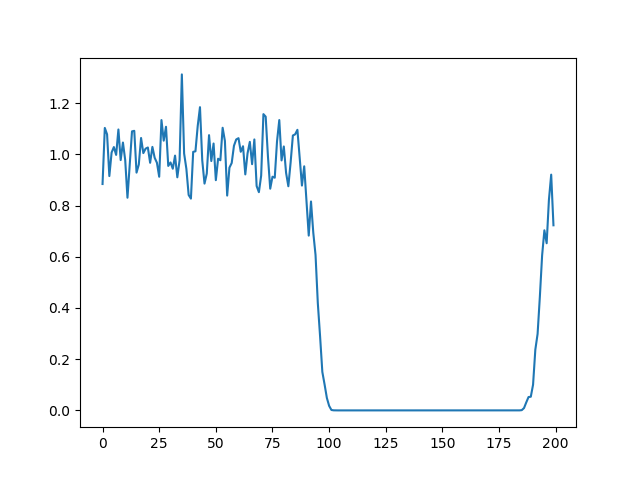
\includegraphics[scale=0.4]{water_density_profile}
\caption{Density of water component across 200 bins in the interface normal direction.}
\end{figure}

We then fit to the error function profile as described in Patel et. al (2006), and obtain the following parameters: $\rho_W = 0.997, h_W = 94.212, w_c = 1.87 Angstroms$, which is in good agreement with previous simulations and experiments.  A plot of the fit is shown below: 

\begin{figure}[H]
\centering
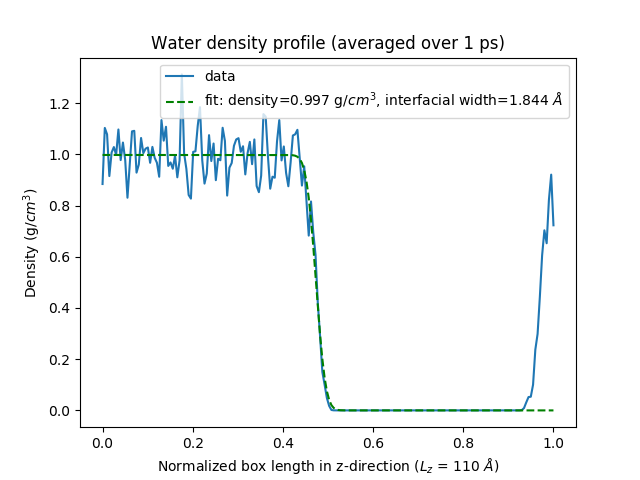
\includegraphics[scale=0.4]{water_density_profile_fit}
\caption{Density of water component across 200 bins in the interface normal direction.}
\end{figure}

\end{enumerate}

\subsection{4/5/2018}

\begin{enumerate}
\item I checked that hexane.in.settings, which contains the intramolecular mixing rules for TAFFI hexane, exhibits Waldman-Hagler mixing:

\begin{align}
\begin{split}
\epsilon_{ij} = 2\sqrt{\epsilon_i\epsilon_j}\left(\frac{\sigma_i^3\dot\sigma_j^3}{\sigma_i^6 + \sigma_j^6}\right)\\
\sigma_{ij} = \left(\frac{\sigma_i^6 + \sigma_j^6}{2}\right)^{\frac{1}{6}}
\end{split}
\end{align}

\item I added the following functionality to interface.py: collecting densities for both water and hexane, and deciding standard versus waldman-hagler mixing, number of equilibration and production steps, the output filenames.  Below is a preliminary figure of combined density profiles taken from just 2000 simulation steps: 

\begin{figure}[H]
\centering
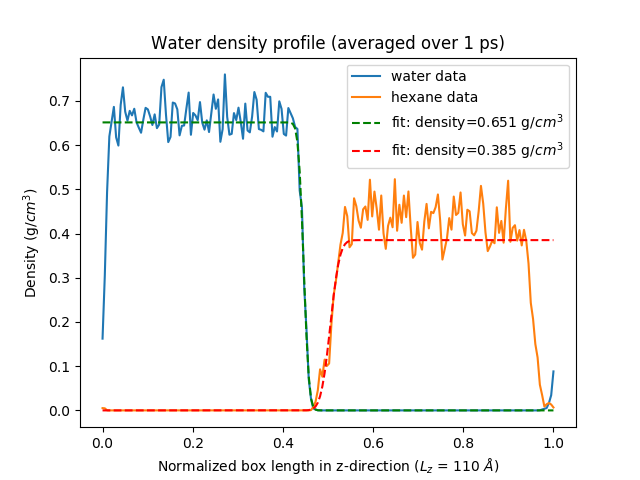
\includegraphics[scale=0.4]{double_profile_test}
\caption{Double density profile test.}
\end{figure}

\item I am now running : DASH simulation of 500 TAFFI hexane, 3650 TIP4P/F water, standard mixing, NPT Andersen/Berendsen at T = 298.15 K and P = 1.0 atm, 300,000 timesteps of length 0.5 fs equilibration followed by 100000 production steps of length 0.5 fs, NPT pre-equilibration of each slab at 298.15 K and same P.  Cutoff = 12.0, Ewald summation.  Classical simulation, no path integrals.  During production run, computing density of water in 200 parallel slabs along the z-direction every 100 simulation steps.  

\item For waldman, I am now running the same as above except waldman mixing, 400,000 equilibration steps only 1000 production, no density calculation.  

\end{enumerate}

\subsection{4/9/2018}

\begin{enumerate}
\item Finished the following run: DASH simulation of 500 TAFFI hexane, 3650 TIP4P/F water, standard mixing, NPT Andersen/Berendsen at T = 298.15 K and P = 1.0 atm, 300,000 timesteps of length 0.5 fs equilibration followed by 100000 production steps of length 0.5 fs, NPT pre-equilibration of each slab at 298.15 K and same P.  Cutoff = 12.0, Ewald summation.  Classical simulation, no path integrals.  During production run, computing density of water in 200 parallel slabs along the z-direction every 100 simulation steps.

\item Problem: After step 300400, i.e. after 400 production steps, the program quits with a "segmentation fault" error.  

\item Although there were only three datapoints, nevertheless it is worth pointing out that the system was able to collect both water and hexane densities.  Using the density profile analysis script, we obtain the following plot of the profile over the first 400 production steps: 

\begin{figure}[H]
\centering
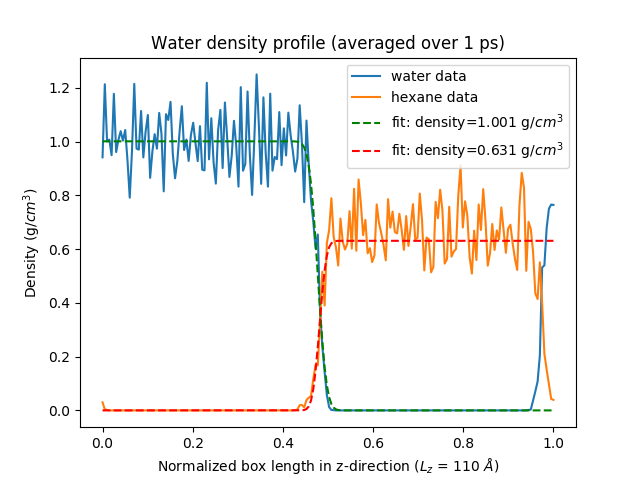
\includegraphics[scale=0.4]{double_profile}
\caption{Double density profile after 400 production steps as described above.  Densities and profiles look reasonable.}
\end{figure}

\item Also ran the same as above excep using waldman mixing, 400,000 equilibration steps only 1000 production, no density calculation.  Here is a plot after the whole simulation:

\begin{figure}[H]
\centering
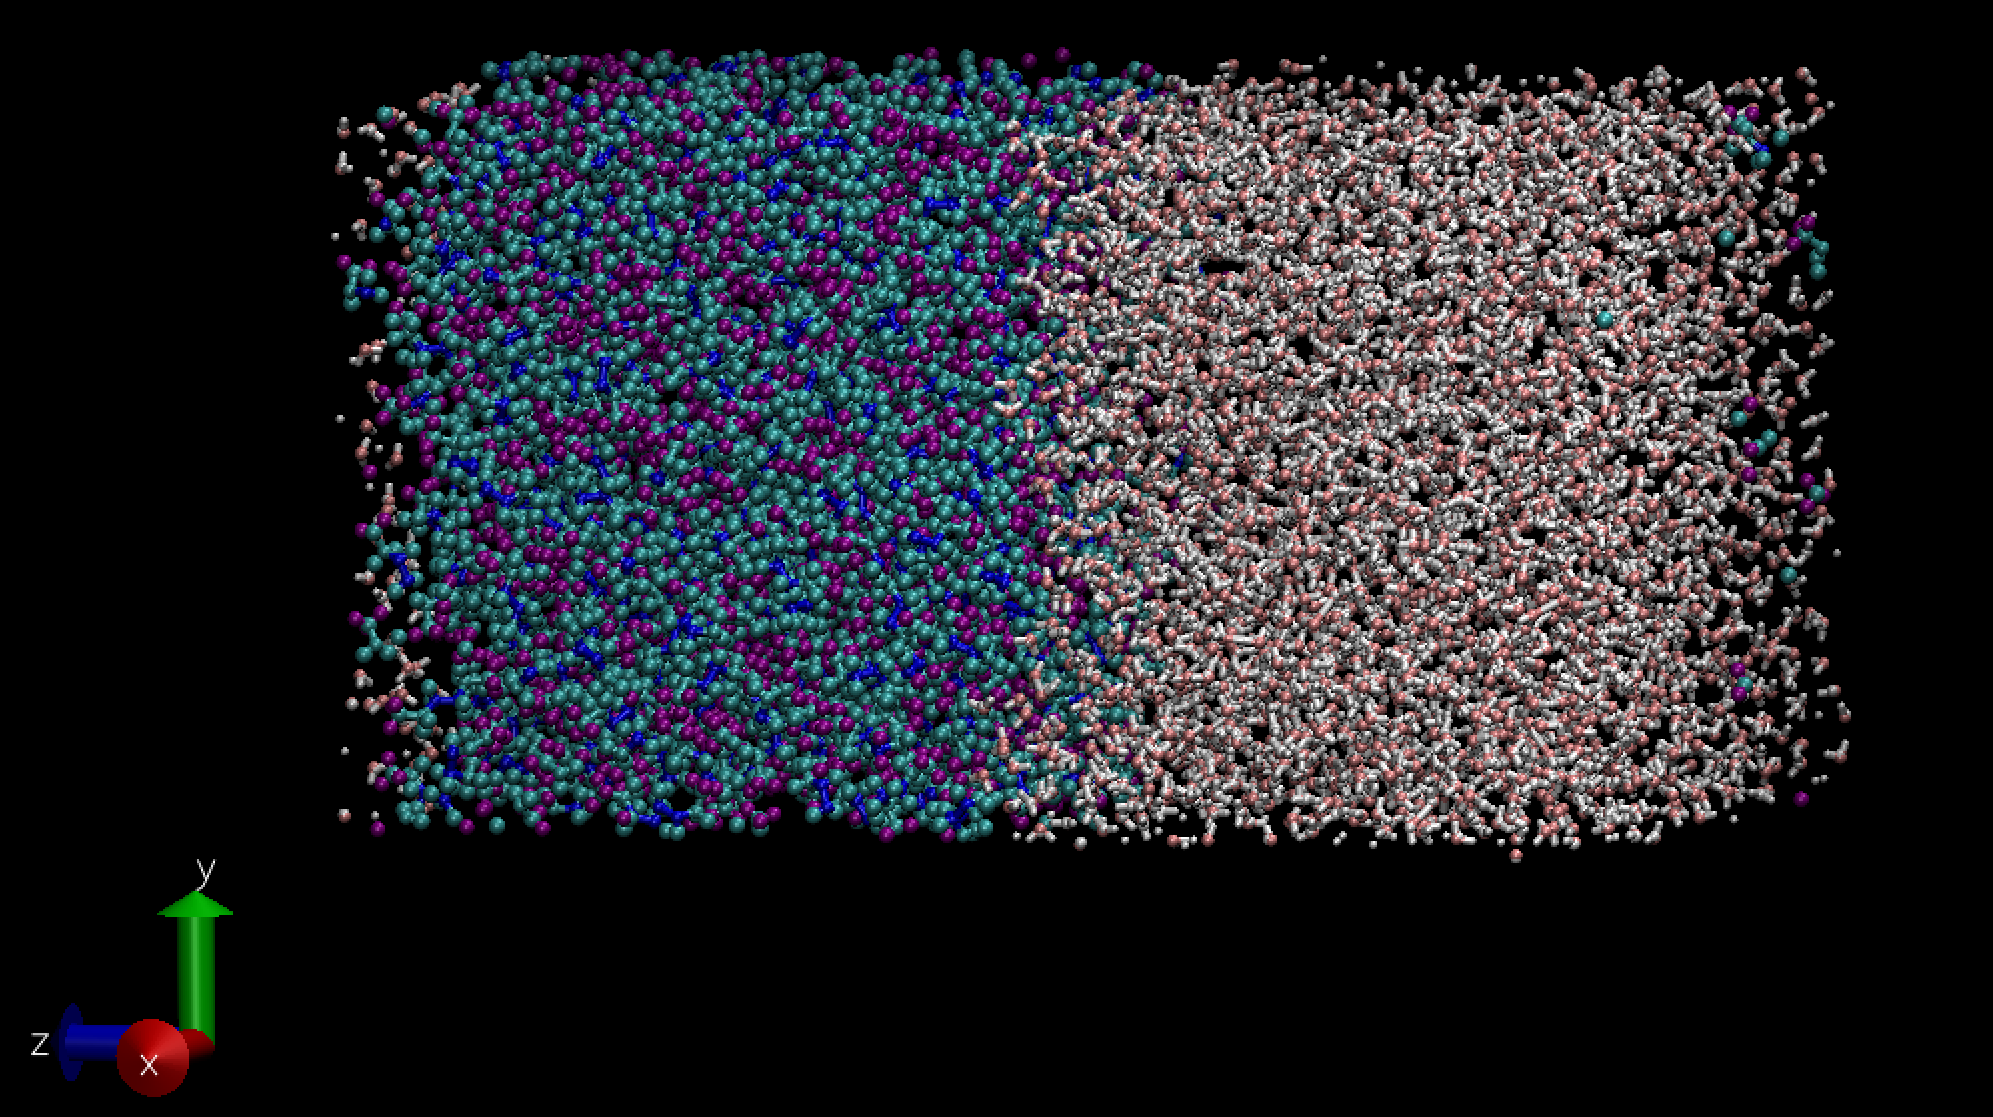
\includegraphics[scale=0.4]{waldman_pic}
\caption{Final snapshot of simulation as described above with Waldman-Hagler mixing.  Looks reasonable.}
\end{figure}

\item From now on we will use W-H mixing.  However, there is still the problem of segmentation fault.  So, we will run three tests o try to discover the origin of this error:
\item Test 1: Run a program that does 300000 pre-equilibration steps and 300000 production steps, no density calculation, see if an error occurs.
\item Test 2: Run a program that does 600000 total pre-equilibration steps and only 1 production step (basically zero production), see if an error occurs, no density calculation.
\item Test 3: Run a program that does 300000 pre-equilibration steps and 300000 production steps, computing the density the whole time. 
\item Test 4: Run a program that does 600000 pre-equilibration steps and 300000 production steps, computing density the whole time.   

\item For the sake of not repeating information, until I note otherwise, all DASH interfacial simulations have the following properties: 500 TAFFI hexane, 3650 TIP4P/F water, waldman-hagler mixing, NPT Andersen/Berendsen at T = 298.15 K and P = 1.0 atm, timestep 0.5 fs, NPT pre-equilibration of each slab at 298.15 K and same P.  Cutoff = 12.0, Ewald summation.  Classical simulation, no path integrals. 

\item Test 1: Running it now.  
\item Test 2: Running now.  
\item Test 3: Running now.  

\item We also want to test density as a function of temperature for the pure hexane and pure water systems.  Let's start with hexane.  In in.webb\_hexane.py, added a final line that computes the standard deviation as well as mean of list of densities.  Mean and sd are computed for the last 500 recordings of density.  Ran lammps\_replicator script to produce input.txt script of initial 500 molecule hexane lattice.  Running DASH system with 500 TAFFI molecules, W-H mixing, NPT Andersen/Berendsen at T = 298.15 K and P = 1.0 atm, timestep of 1 fs, cutoff = 10, 2,000,000 steps.  Density is calculated every 100 steps, and the mean and sd calculations below represent the last 500 recordings, or 50,000 steps.  

\item T = 298.15 K, $\rho = 0.65166 g/ml$, $\sigma = 0.0004788 g/ml$, expt: 0.65478 $g/ml$ on NIST Chemistry Webbook at P = 1.0 atm.  So, the density is off by -0.476\%.  
\item T = 320 K, $\rho = 0.62475 g/ml$, $\sigma = 0.00072859 g/ml$, expt: 0.63434 $g/ml$.  So, the density is off by -1.5118\%.  
\item T = 270 K, $\rho = 0.68196 g/ml$, $\sigma = 0.000927 g/ml$, expt: 0.68025 $g/ml$.  So, the density is off by +0.25\%.  


\item Now we will move onto water.  Created a new file in.tip4pF\_dens.py, in which I added the same mean and sd calculations as above.  Time step 0.5 fs, 2,000,000 steps, initial density of 0.997, 3650 molecules, cutoff = 9.0.  Running this now.  

\item T = 298.15K, $\rho = 0.98919 g/ml$, $\sigma = 0.00116 g/ml$, https://webbook.nist.gov/cgi/fluid.cgi?ID=C7732185\&Action=Page expt: 0.99705 $g/ml$ at P = 1.0 atm.  So, the density is off by -\%0.00788.   
\item T = 270K, $\rho = 0.988 g/ml$, $\sigma = 0.001555 g/ml$, but this is below freezing??
\item T = 300 K, $\rho = 0.9877 g/ml$, $\sigma = 0.0034977$, expt: 0.99656.  So, the density is off by -0.00889 \%
\item T = 320 K, $\rho = 0.98157 g/ml$, $\sigma = 0.0022$, expt: 0.989.  So, the density is off by -0.0075\%.  


\item RESULT: Test 1 ran perfectly fine.  300,000 pre-equilibration, 300,000 production, no density calculation, no segmentation fault!  
\item RESULT: Test 2 ran perfectly fine.  600,000 pre-equilibration steps, 1 production step, 1 production step, no density calculation, no segmentation fault!
\item Running test 3 still.  

\item Note: the units for mass in DASH are amu, and the units for distance are Angstroms.  So, we use the conversion factor $\frac{1}{0.6022}$ to convert this to $g/ml$.  

\item Test 4: Same as test 3, but density calc is only every 1000 turns instead of every 100 turns.  This is the REAL test 4, not as described above.    

\item Created an interface\_hexane\_restart.py file that spits out a hexane\_interface\_restart.txt file, and tried constructing an interface\_restart.py file, but resulted in green's function errors.  It creates an initial configuration that looks fine but does not integrate the system.  

 
\item Change densities.txt file names in interface.py!  
\end{enumerate}

\subsection{4/12/2018}
\begin{enumerate}
\item RESULT: Test 3, program stopped after 107300, 35.77 \% done, Fatal Python error: GC object already tracked.  /tmp/slurmd/job44973736/slurm\_script: line 30: 12701 Aborted.  Computing densities every 100 steps.  
\item RESULT: Test 4, program stopped after 112300, 37.43 \% done, computing density every 1000 steps.  Segmentation fault error.  
\item Ok, in order to diagnose this problem, let's run more tests.  

\item Test 5: 300,000 preequilibration steps, 300,000 production steps, density profile function computing density every 1000 steps is there but not activated in the sbatch script.
\item Test 6: Same as test 5, except actually computing the density as usual every 1000 steps.
\item Test 7: Same as above, except the density profile does not actually comput anything.
\item Test 8: Same, except density function only active up to the loop.
\item Test 9: Same, except density function only active up to the first write file command.  
\item Test 10: Same, except density only active until last write file.
\item Hopefully, these tests will dig into the details of excactly where the issue is arising.  
\item Sent a message to Brian about this issue, and got a response saying I should try "In your PythonOperation() constructor in the python script, did you set synchronous=True?  If not, I would try that.  The default behavior is asynchronous."  So, before running all of these tests, I will try this first!
\item In the file for test 5, called interface\_test5.py, I made this change to PythonOperation().  Let's try this now. 
\item It appears to be working.  Modified the original interface.py to reflect this, as well as customizing filename for the density files.  Currently running DASH simulation of the interface using 400,000 preequilibration steps, followed by 300,000 production steps during which density profiles are measured every 100 steps.   
\end{enumerate}

\subsection{4/17/2018}

\begin{enumerate}
\item What we really need is to do post-production.  So, for the successful run above, we are just going to take the trajectory file and analyze that.  In this case, the file is interface-dens.xyz.  
\end{enumerate}

\subsection{4/18/2018}

\begin{enumerate}
\item Here are the results from our analysis: 

\subitem Bulk water density: 0.999247086118 $g/cm^3$
\subitem Bulk hexane density: 0.674945918949 $g/cm^3$
\subitem Intrinsic width: 0.712788562077 Angstroms
\subitem Water thermal width: 1.89474070104 Angstroms
\subitem Hexane thermal width: 1.85287262473 Angstroms

\begin{figure}[H]
\centering
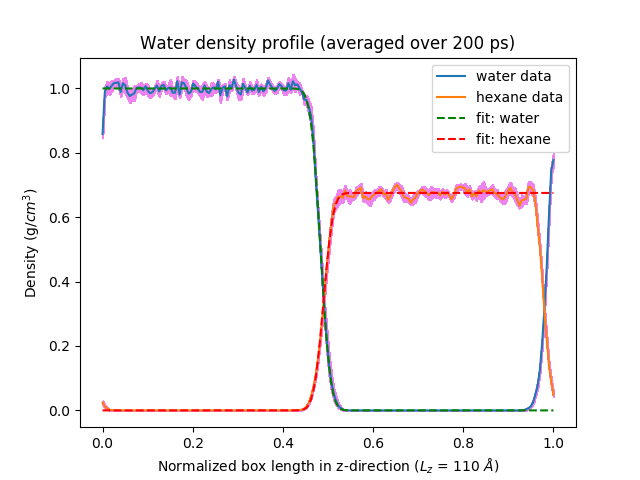
\includegraphics[scale=0.4]{double_profile_with_errors}
\end{figure}

\item Based on inspection, the average box length in the z-direction is assumed to be 110.0 Angstroms.  Also based on visual inspection of the profiles, the bulk region for water is determined to be 0.1 < z < 0.4, while the bulk region for hexane is 0.6 < z < 0.85.  The bulk densities for each are computed in those respective regions.  The curve fits for error function profiles, described in Patel and Brooks 2006, are fit using scipy curve\_fit function, where the bulk densities are specified but not the Gibbs dividing surfaces or the thermal width.  The widths are left to be separate.  The fits are done only in the interfacial region of the data, which is determined by inspection to be 0.4 < z < 0.6.  The standard error measurements are performed by dividing the 200 ps data into 5 blocks, and finding the SE of the mean across all 200 bins over which the averaeg profiles are computed.  The result of the SE is shaded in pink for each profile.  

\item We will now run a simulation that computes 300,000 equilibration steps and 1,000,000 ps production.  The system will be NPT in equilibration, but then immediately fixed to NVT in production.  No density calculation.  Although it would be optimal to calculate the average box length after equilibration and then set V to that box length, for now we will skip that step.  NVT is to ensure that we have fixed bins over which to compute density profiles.  The python script will be named interface\_NVT.py.  


\end{enumerate}

\section{4/22/2018}

\begin{enumerate}
\item Wrote python script, molecular\_orientation\_postproduction.py that computes $S_{zz}$ in 200 slabs, and then orientation\_profile\_analysis.py that averages and plots them.  Here is the result for water:

\begin{figure}[H]
\centering
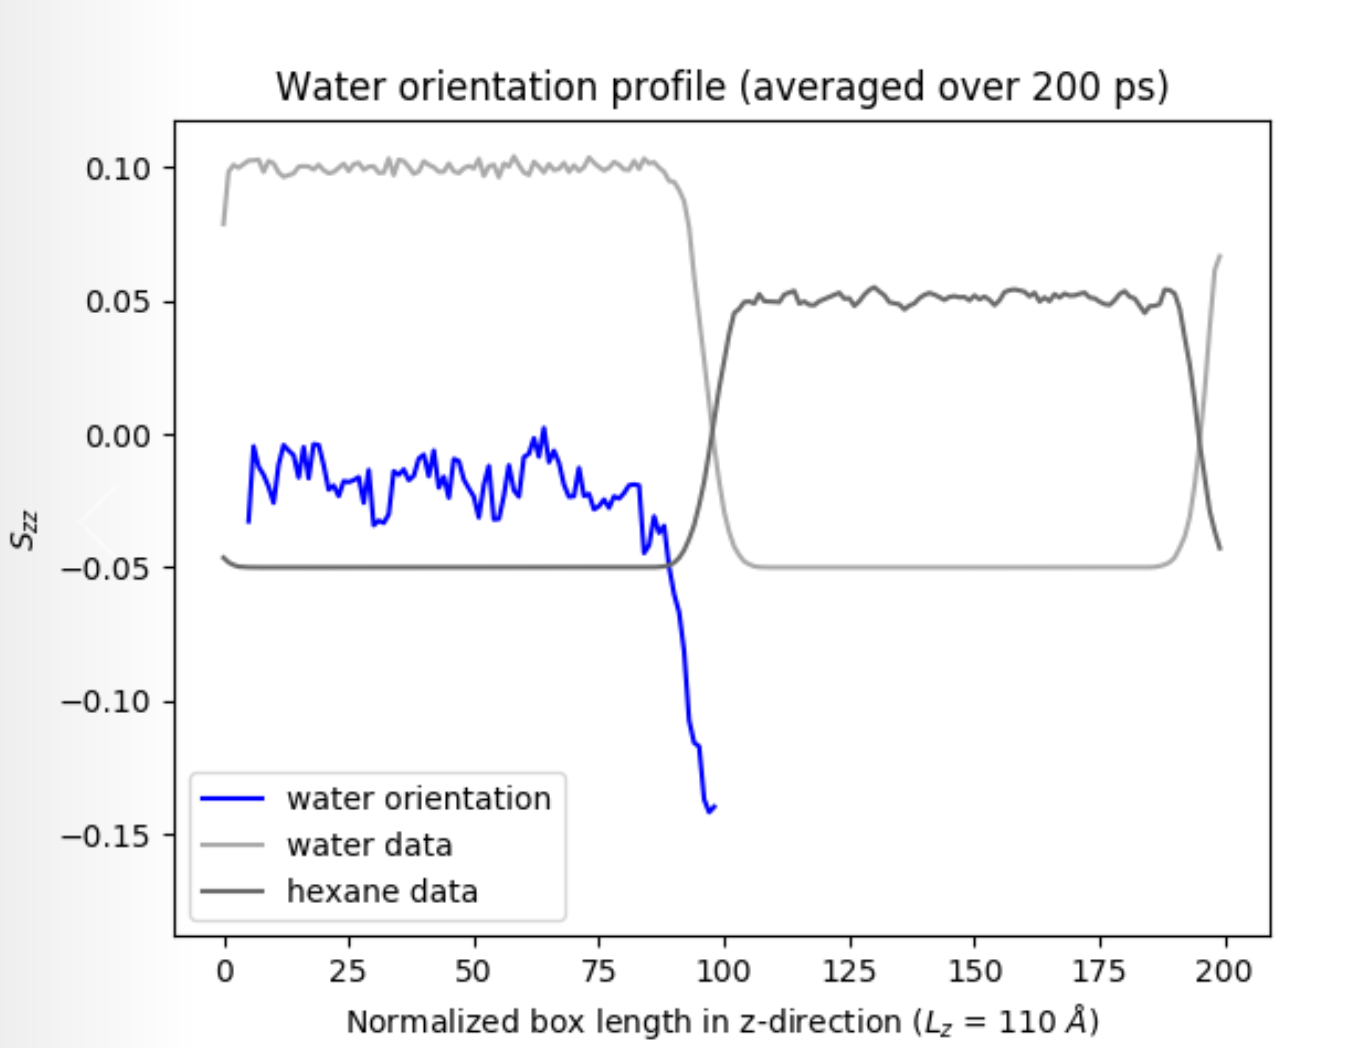
\includegraphics[scale=0.4]{water_orientation}
\end{figure}

which compares favorably to one of the models discussed in Patel and Brooks (2006):
\begin{figure}[H]
\centering
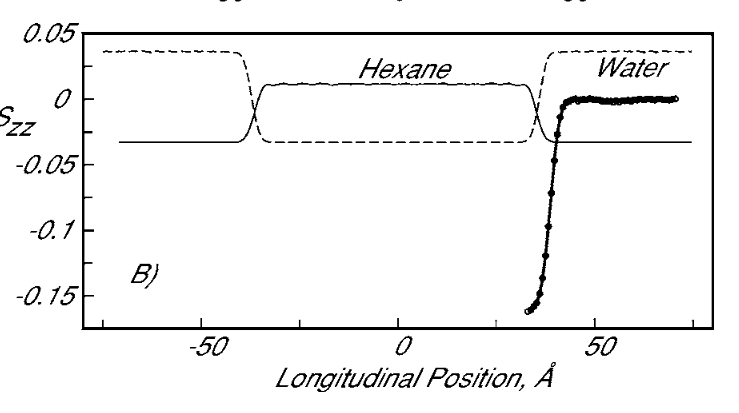
\includegraphics[scale=0.4]{patel_water_orientation}
\end{figure}

These results indicate that water dipole moment is isotropic in the bulk, but orients preferentially along the interface in the interfacial region.  For hexane, we see:

\begin{figure}[H]
\centering
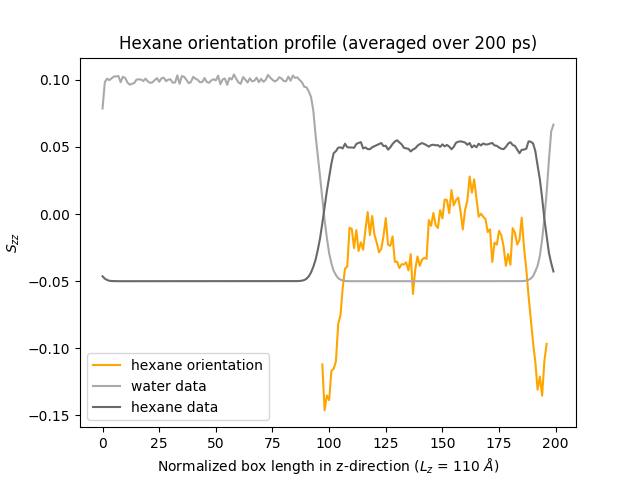
\includegraphics[scale=0.4]{orientation_hexane}
\end{figure}

This also matches with Patel:

\begin{figure}[H]
\centering
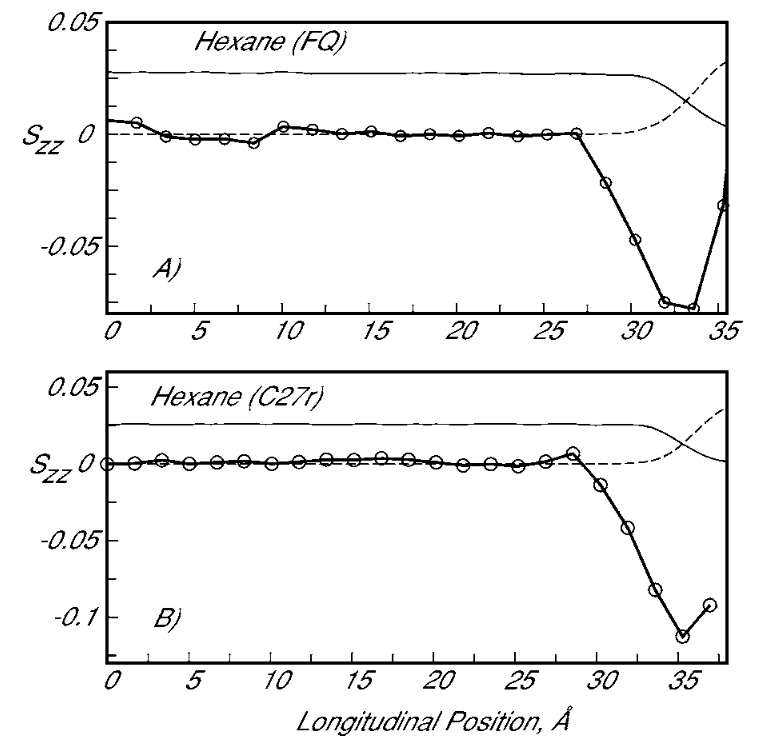
\includegraphics[scale=0.4]{patel_hexane_orientation}
\end{figure}



\end{enumerate}

\subsection{4/23/2018}

\begin{enumerate}
\item Compiled latest version of DASH, placed in /home/swansonk1/NEW\_DASH.  Copied the water.py from utils.py in OLD\_DASH.  Everything seems to run smoothly, including restart files!  
\item So now, we will run the file interface\_new.py, which has the link to new dash.  We will do 400,000 steps (i.e. 200 ps) of equilibration.  Prints restart file every 10,000 steps.  Run file is run\_new.sh.    
\end{enumerate}

\section{4/24/2018}

\begin{enumerate}
\item Trajectory data for interface\_NVT.py is contained in interface-NVT.xyz.  
\item The first thing we want to do is to construct a production run dataset that has path integrals.  We used interface\_new.py and run\_new.sh to perform a 400,000 step (i.e. 200 ps) equilibration in NPT using the standard parameters.  Now, we will restart that simulation, except we will use path integral beads.  As proof of concept, we will start with just a few, say 16 beads.  The DASH script will be called interface\_restart\_new.py, and the sbatch will be run\_restart\_new.py.  The restart input file will be equilibration400000.xml.  
\item Ok, it appears as though restart works perfectly fine using path integrals.  Setting number of beads to 16 and doing a run of 200,000 steps, i.e. 100 ps, under NVT conditions.  We will use this to generate a preliminary dataset.  
\end{enumerate}

\section{4/25/2018}

\begin{enumerate}
\item Based on Patel and Brooks (2006) and the sources they cite, the interfacial tension can be computed as 

\begin{align}
\begin{split}
\gamma = \frac{L_{zz}}{2}\left[\left<P_{zz}\right> - \frac{1}{2}\left(\left<P_{xx}\right> + \left<P_{yy}\right>\right)\right], 
\end{split}
\end{align}
where $P_{\alpha\beta}$ are computed from the standard definition of the atomic virial.  From Tildesley's computer simulation of liquids, this is defined as:

\begin{align}
\begin{split}
P_{\text{instantaneous}} = \rho k_B T + W/V, 
\end{split}
\end{align}

where $W$ can be written as:

\begin{align}
\begin{split}
W = -\frac{1}{3}\sum_i\sum_{j > i}\textbf{r}_{ij}\cdot \textbf{f}_{ij} = -\frac{1}{3}\sum_i\sum_{j > i}w(r_{ij}) \\
w(r) = r\frac{dv(r)}{dr}.  
\end{split}
\end{align}

In "Molecular dynamics simluation of the orthobaric densities and surface tension of water", by Alejandre, Tildesley, and Chapela, the authors note the following.  Similar to the above definition of the pressure tensor elements and atomic virial, the elements $\alpha\beta$ of the molecular pressure tensor can be written as:

\begin{align}
\begin{split}
VP_{\alpha\beta} = \sum_{i = 1}^Nm_i(\textbf{v}_i)_\alpha(\textbf{v}_i)_\beta + \sum_{i = 1}^{N - 1}\sum_{j > i}^N\sum_a\sum_b(\textbf{r}_{ij})_\alpha(\textbf{f}_{iajb})_\beta, 
\end{split}
\end{align}

where N is the number of molecules, V is the volume, $m_i$ and $\textbf{v}_i$ are the molecular mass and velocity of the center of mass, respectively, $\textbf{r}_{ij}$ is the vector between the center of mass of molecules $i$ and $j$ and $\textbf{f}_{iajb} = -\frac{\textbf{r}_{iajb}}{r_{iajb}}\left[\frac{dU(r_{iajb})}{dr_{iajb}}\right]$ is the force between atom $a$ in molecule $i$ and atom $b$ in molecule $j$.  The distance betwen atom $a$ in molecule $i$ and atom $b$ in molecule $j$ is denoted by $r_{iajb}$.  

Although the above definitions used molecular center of mass for calculations, J. G. Harris J. Phys. Chem. 1992 notes that the virial can be calculated using both the molecular and atomic routes.  "Although both the molecular and atomic formulas for the surafce tension should produce equivalent ensemble averages, the instantaneous values and magnitude of flucutations can differ significantly.  The atomic and molecular virial formula do yield different values for the individual $V_{\alpha\alpha}$.  In computing the pressure tensors [however], this difference is offset by the differences in the atmoic and molecular kinetic terms."  \\

The Tildesley paper goes on to note that "The definition of the molecular pressure tensor in Eqn. (4) is only valid for additive potentials and the calculation of $\textbf{f}_{iajb}$ and hence $P_{\alpha\beta}$ is in general simple.  The constraint forces and the forces arising from bond-angle distortions make no contribution to the molecular pressure tensor.  In the case of the electrostatic interactions treated with the Ewald sum, there are two contributions to the potential, one in the real space (which is pairwise-additive) and other in the reciprocal space (which is not).  In the latter case Eq. (4) is not applicable and the appropriate expression is given in Appendix A."\\

However, after talking to Dan and Brian, we realize that the pressure tensor elements can be computed directly in DASH during a simulation, and that these elements appropriately account for long-range electrostatic contributions from the Ewald method.  

\item So, now we will create a new simulation, that starts from the 400,000 step equilibration and computes pressures directly every 1000 steps.  We will start with interface\_restart\_new.py, comment out the path integral stuff, and then add pressure tensor computations.

\item Wrote tension\_analysis.py to evaluate the interfacial tension.  Getting values around 200 or 300 mN/m though, so not sure what is going on here.  Will have to evaluate further at another time.  

\item Running PI-1, which is 200,000 steps (100 ps) under NVT conditions but only 1 bead this time.  We will use this information to compare results and see if there is any differences!!  

\item Here are the results for 200,000 NVT steps after the 400,000 NPT equilibration with 1 bead:
\subitem Bulk water density: 0.999555449512 $g/cm^3$
\subitem Bulk hexane density: 0.668818766515 $g/cm^3$
\subitem Intrinsic width: 0.735859948359 Angstroms
\subitem Water thermal width: 1.78265926051 Angstroms
\subitem Hexane thermal width: 1.73435836695 Angstroms

\begin{figure}[H]
\centering
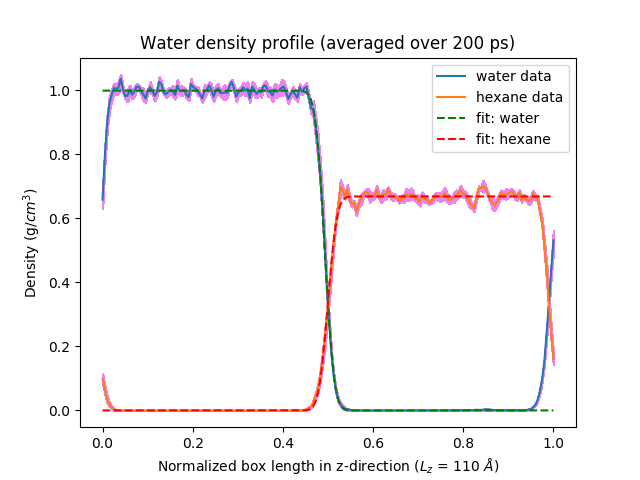
\includegraphics[scale=0.4]{interface_density_profile_PI-1}
\end{figure}

\section{4/26/2018}

\begin{enumerate}
\item Here are the results for 200,000 NVT steps after the 400,000 NPT equilibration with 16 beads:
\subitem Bulk water density: 1.00165502632 $g/cm^3$
\subitem Bulk hexane density: 0.665009086668 $g/cm^3$
\subitem Intrinsic width: 0.694754973486 Angstroms
\subitem Water thermal width: 1.56257576587 Angstroms
\subitem Hexane thermal width: 1.49811476734 Angstroms
\end{enumerate}

\begin{figure}[H]
\centering
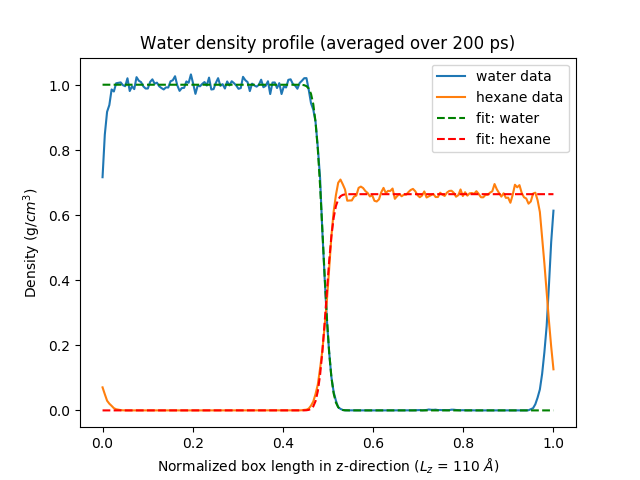
\includegraphics[scale=0.4]{interface_density_profile_PI-16}
\end{figure}

\item Surace tension def'n:   

\end{enumerate}



\section{4/30/2018}

\begin{enumerate}
\item Removing an error pointed out by Mike in the PIMD code.  Instructions from Mike: open up IntegratorVerlet.cu, remove lines 137 and 138, because reduceByN is redundant.  Doing this in the NEW\_DASH file.  
\item Modified interface\_restart\_new.py such that there are 16 beads and no pressure tensor computations.  We will run this through run\_restart\_new.sh to check if the modification to the PIMD code messed anything up.  File will be PIMD-test.  10,000 steps. 
\item How to compute statistical uncertainty in measurements?
\item Also forgot to log this, but Dan made a fix to the pressure tensor recording, in src/DataStorageUser/DataComputer/pressure.cu, issue with converting C++ to python list or something.  This was also compiled earlier.  
\item Realized I did not compile the Mike fix, so compiling then checking again.  
\item Still, everything looks fine.  
\item Mike found another error in src/GridGPU.cu.  The line wrapping centroids was missing from part of the code.  
\end{enumerate}

\section{5/1/2018}

\begin{enumerate}
\item First, we will set up a rigorous simulation of the classical system.  We will do this by looking at the 400,000 NPT equilibration steps in the file equilibration.xyz, which is the system we have been taking restart trajectories from.  We will first plot the box volume to see how it varies over time.  

\begin{figure}[H]
\centering
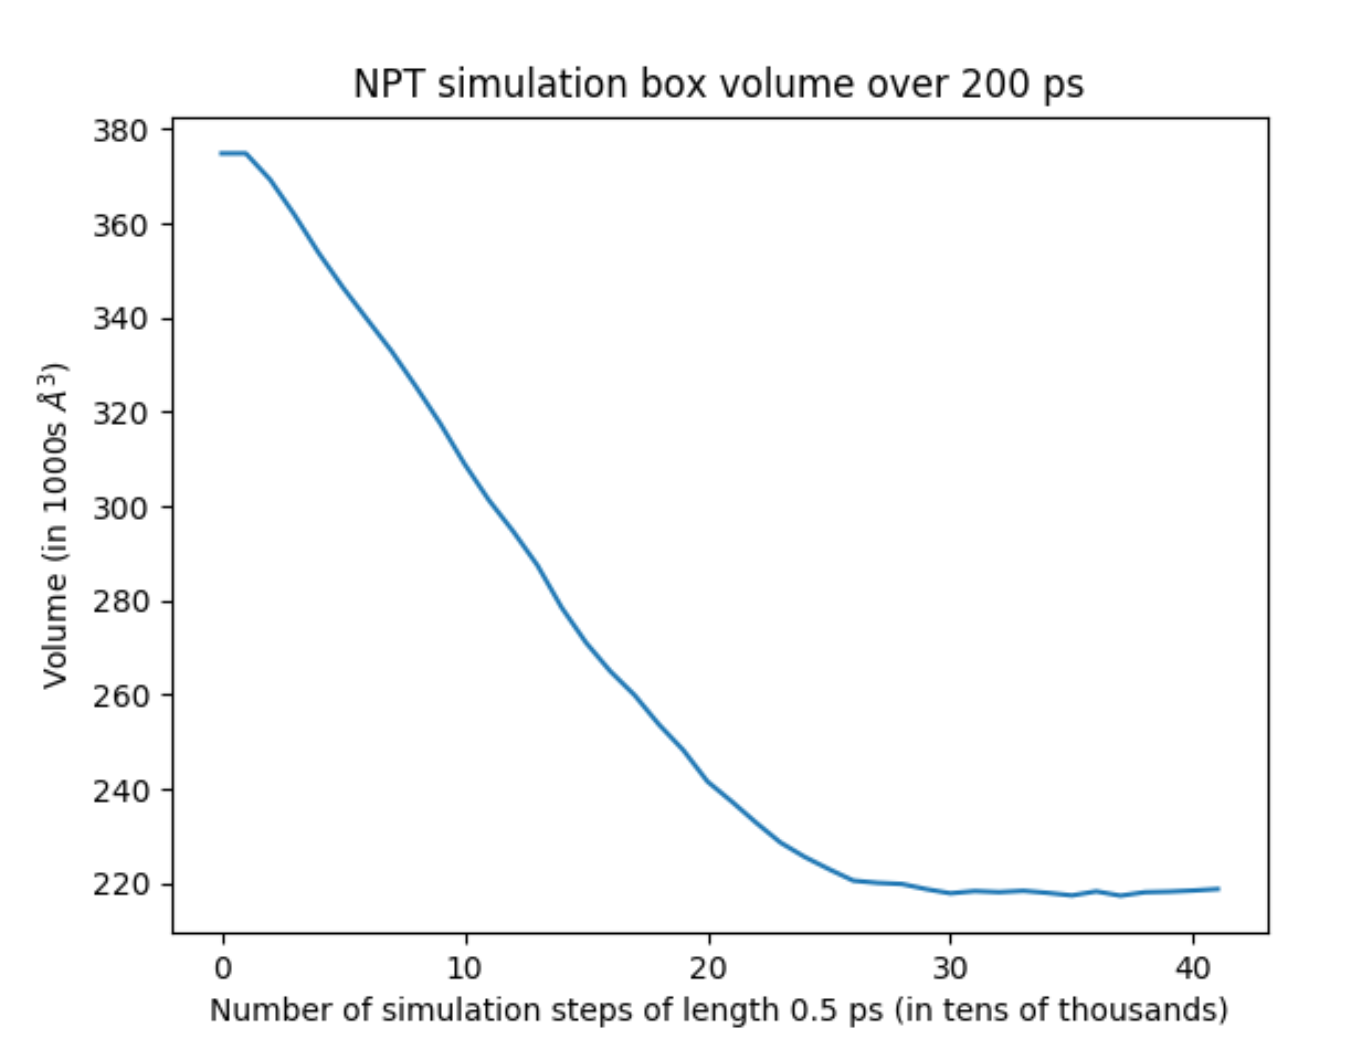
\includegraphics[scale=0.4]{NPTvolumes}
\end{figure}

\item It is clear that the box volume equilibrates after 300,000 timesteps.  So, we will check the average box dimensions in the last 50 ps of the simulation:  
\subitem Average x-length: 48.80
\subitem Average y-length: 48.99
\subitem Average z-length: 91.23

\item The restart file we are using, equilibration400000.xml, gives the following box length values:

\subitem Restart x-length: 48.85
\subitem Restart y-length: 49.04
\subitem Restart z-length: 91.32

\item Let's see if we can adjust the starting volume at all.  Increased the bounds\_xlo by 0.05, increased the bounds\_ylo by 0.05, and increased the bounds\_zlo by 0.09 in order to change box side lengths to average values.  Simulation appears to be running.  SO, we will now run the restart classical 0 beads simulation NVT.  Filename "trueNVT", 2,000,000 steps.  With the changed initial bounds.  This is running now.
\item Now going into run\_new.sh and interface\_new.py files.  We are going to try running a 1 bead simulation, STARTING from NVT conditions.  We will run this for 1,000,000 timesteps and see what happens, i.e. check if the system equilibrates or not.  This is running now.

\end{enumerate}

\section{5/2/2018}

\begin{enumerate}
\item We ran a 1 bead NVT simulation for 1,000,000 timesteps, where we subtracted and added 20 Angstroms from the z lo and z hi dimensions, respectively.  The DASH script was named interface\_new\_NVT.py  Here is an image of the final configuration:

\begin{figure}[H]
\centering
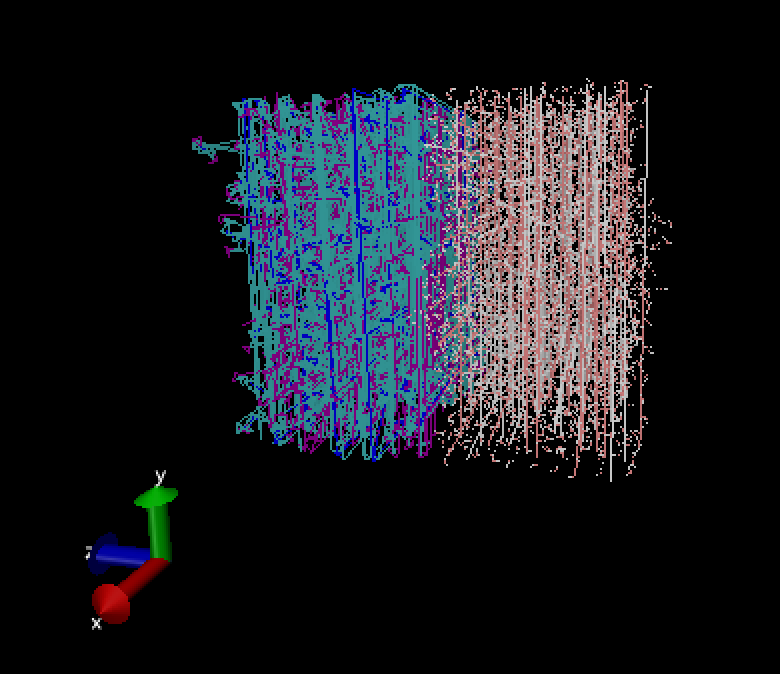
\includegraphics[scale=0.4]{wide-NVT-1bead}
\end{figure}

\item It looks possibly reasonable.  We also ran a 1 bead NVT simulation for 1,000,000 timesteps with the minimal box volume.  Here is an image of the final configuration:

\begin{figure}[H]
\centering
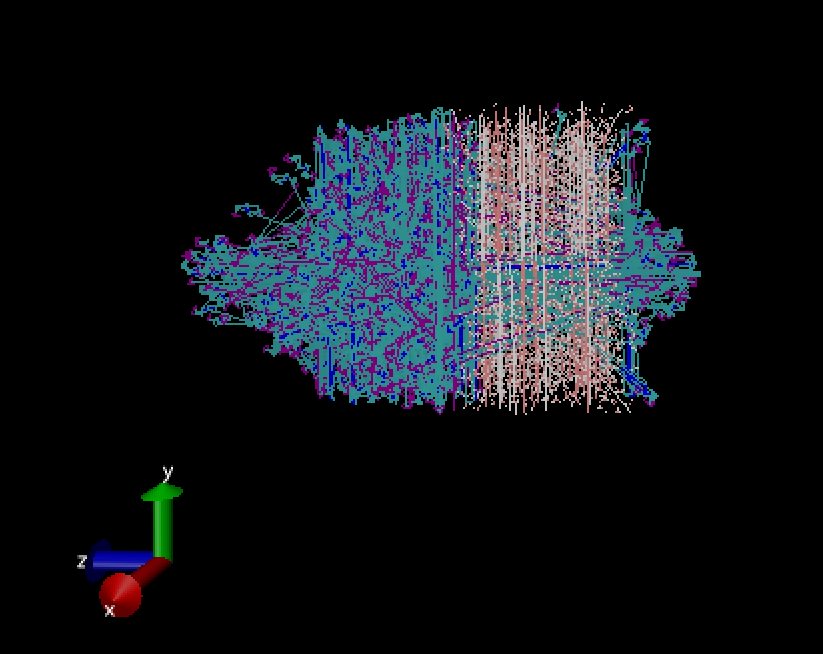
\includegraphics[scale=0.4]{original-NVT}
\end{figure}

\item So, it looks like providing extra space is important...

\item Ok, so based on this, let's do three more simulations.  The first will be similar to what we just did with the extra space, but with 16 beads as well as 32 beads.  
\item Changed interface\_new\_NVT.py to have 16 beads.  Using run\_new.sh to do the NVT equilibration simulation for 1,000,000 steps with files named NVTequil-16bead.
\item The second is: creating a new file named interface\_new\_NVT32.py which will have 32 beads.  Doing the same as above, file named NVTequil-32bead.  This has been submitted to run.  
\item The third will be to restart from the apparently successful simulation with 1 bead with the expanded NVT volume.  We will use the restart file NVTequil-1bead-new990000.xml.   The filename will be NVTprod-1bead.  We will do 2,000,000 production steps, i.e. 1 ns.  This has been submitted to run.

 

\end{enumerate}

\section{5/3/2018}

\begin{enumerate}
\item Did density\_profile\_postproduction.py on the bigmem partition for the trueNVT 2,000,000 classical steps.  Needed more memory.  Ok, now we will download densities\_water\_trueNVT.txt and hexane equivalent to laptop to perform analysis.   
\item We will again use density\_profile\_postproduction.py on bigmem for NVTprod-1bead.xyz data to get density profile info.  Files called densities\_water\_NVTprod-1bead.txt.
\item Now, we are going to use the restart file NVTequil-32bead-990000.xml.  The filename will be NVTprod-32bead.  We will again do 2,000,000 production steps, i.e. 1 ns.  
\item Problems with the restart file.  So, we will run simulations that include both equilibration and production steps.  In other words, we will run NVTequil-16bead-long and NVTequil-32bead-long, which will each be run for 3,000,000 steps!  dayum.  Both running now.
\end{enumerate}


\section{5/4/2018}

\begin{enumerate}
\item 1.  We ran an NVT classical 2,000,000 timestep simulation restarting from the NPT equilibration run with the box dimensions adjusted so that the reflect the average equilibrated volume (see above).  We then ran density\_profile\_postproduction.py on bigmem to produce the files densities\_water\_trueNVT.txt and densities\_hexane\_trueNVT.txt, which we downloaded to laptop.  We then used density\_profile\_analysis.py to analyze these profiles.  Similar to previous analysis, we assumed that the water bulk was 0.1 < z < 0.4 and the hexane bulk was 0.6 < z < 0.85.  This time, we have the exact box length in the z direction, 91.234905 Angstroms.  Using the entirety of the available data, and the computed bulk water and hexane densities, we performed separate fits of water and hexane density profiles to obtain a "total intrinsic width" and a "total thermal width."   We then added functionality to perform a simultaneous fitting, which uses the individual fits to provide initial estimates for the Gibbs dividing surfaces of hexane and water as well as the water width as an estimate for the joint thermal width.  It also uses the bulk densities as hard-coded values.  The simultaneous fitting then performs a least squares optimization to give the total width values, which are close to the original individual fits.  Finally, we compute the "intrinsic width" and the "thermal width."  We split the data into 5 sections, i.e. 5 200 ps intervals.  For each block, we compute the simultaneous fitting of the intrinsic and thermal widths, using the average density values from that specific block.  We then report the mean of these fits as well as the standard error of the mean for these fits, which we report below.  Finally, SE of the mean density profiles across the 200 slabs are also shown in the plot in purple.   

\begin{align}
\begin{split}
\text{bulk water density: } 1.00047355545 \\
\text{bulk hexane density: } 0.672799468906 \\
\text{separate fitting intrinsic width: } 0.588579658835 \\
\text{water thermal width: } 1.64305504711 \\
\text{hexane thermal width: } 1.58958186287 \\
\text{total intrinsic width: } 0.587937486508 \\
\text{total thermal width: } 1.62624544958 \\
\text{block-averaged intrinsic width: } 0.61996503417 \pm 0.0132678744671 \\
\text{block-averaged thermal width: } 1.37899476187 \pm 0.0323005854543 \\
\end{split}
\end{align} 

Here is the plot for individual fits using the entire data at once (NOTE THAT THE X-AXIS HAS WRONG LABEL):

\begin{figure}[H]
\centering
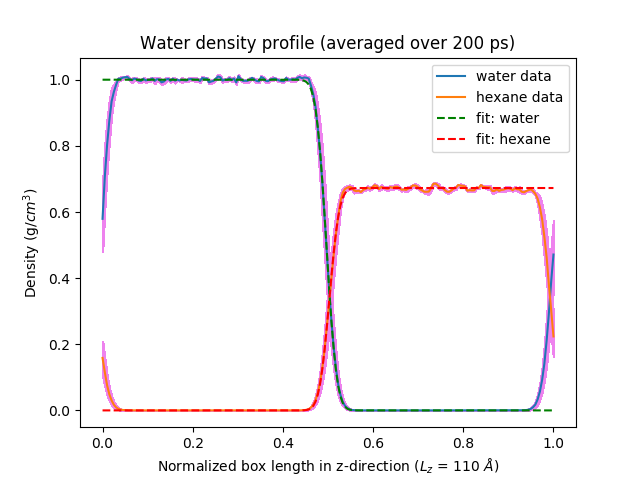
\includegraphics[scale=0.6]{interface_density_profile_individualfit_trueNVT}
\end{figure}

Here is the plot for simultaneous fit using the entire data at once:

\begin{figure}[H]
\centering
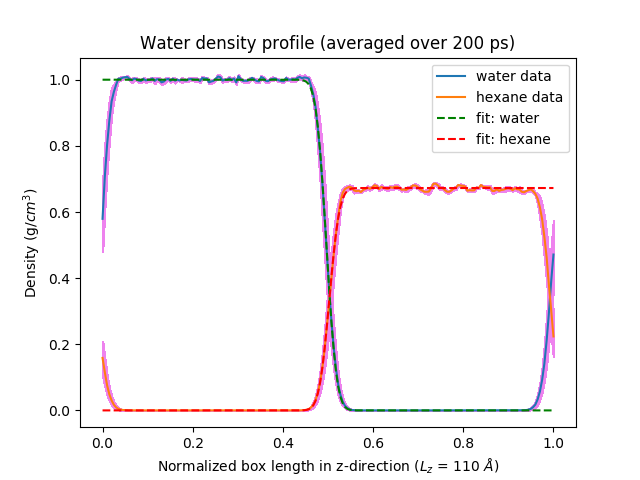
\includegraphics[scale=0.6]{interface_density_profile_simultaneousfit_trueNVT}
\end{figure}

Here is the plot for simultaneous fit using block averaging technique (i.e. parameters are averages of simultaneous fits from the 5 blocks): 

\begin{figure}[H]
\centering
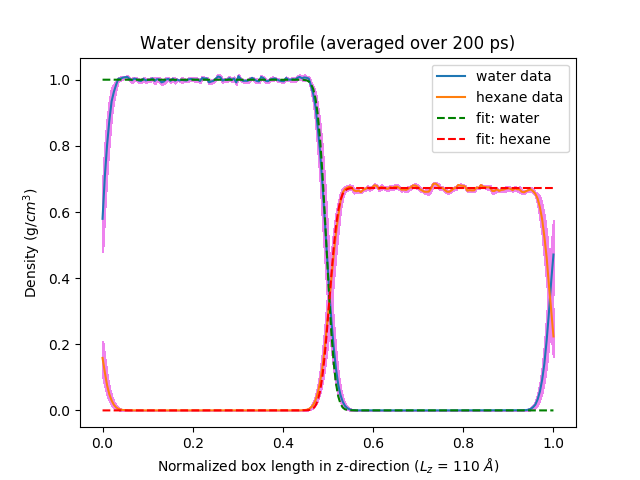
\includegraphics[scale=0.6]{interface_density_profile_blockfit_trueNVT}
\end{figure}

Issues to note here are that the total width values do not fall within the SE estimate for the widths, which might indicate that the block size or number of blocks is erroneous.  Also, the width values are interesting, thermal width seems small.  \\

We also analyzed the pressure tensor file, pressure\_tensorstrueNVT.txt, and it gave an average interfacial tension of  77.43.  Well, this is quite off, but at least the larger tension is related to a smaller interfacial width...

\item 2.  We are now going to check the results from the following: equilibration using an EXPANDED box, i.e. equilibration in NVT for 1,000,000 timesteps, followed by 2,000,000 NVT production steps using a restart file (which apparently works for 1 bead).  We have used density\_profile\_postproduction.py on bigmem for NVTprod-1bead.xyz data to get density information, which we downloaded.  The files are called densities\_water\_NVTprod-1bead.txt and densities\_hexane\_NVTprod-1bead.txt.  We will now use density\_profile\_analysis.py to produce results on these and compare with the NPT-NVT classical result.  \\

Here is the plot of the density profiles:

\begin{figure}[H]
\centering
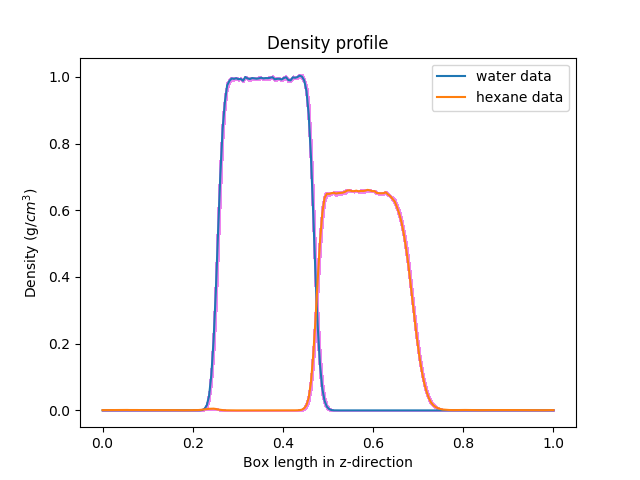
\includegraphics[scale=0.6]{interface_density_profile_NVTprod-1bead}
\end{figure}

Based on this plot, we will estimate that the bulk water region is in 0.3 < z < 0.4, the interfacial region is 0.4 < z < 0.55, and the bulk hexane region is 0.55 < z < 0.62.  So, we will change the code to reflect this.  The x length is 58.45467 Angstroms, y length is 58.67825, and z length is 149.2717, based on NVTprod-1bead.xyz. \\

Using the same scheme as above, 


\begin{align}
\begin{split}
\text{bulk water density: } 0.995053633154 \\
\text{bulk hexane density: } 0.656798321085 \\
\text{separate fitting intrinsic width: } 0.649275263102 \\
\text{water thermal width: } 1.61254923014 \\
\text{hexane thermal width: } 1.57211041522 \\
\text{total intrinsic width: } 0.64913333243 \\
\text{total thermal width: } 1.60032720938 \\
\text{block-averaged intrinsic width: } 0.655975139284 \pm 0.0068168498649 \\
\text{block-averaged thermal width: } 1.53323689614 \pm 0.047053357657 \\
\end{split}
\end{align} 

Here are the individual, simultaneous total, and simultaneous block-averaged plots, respectively: 

\begin{figure}[H]
\centering
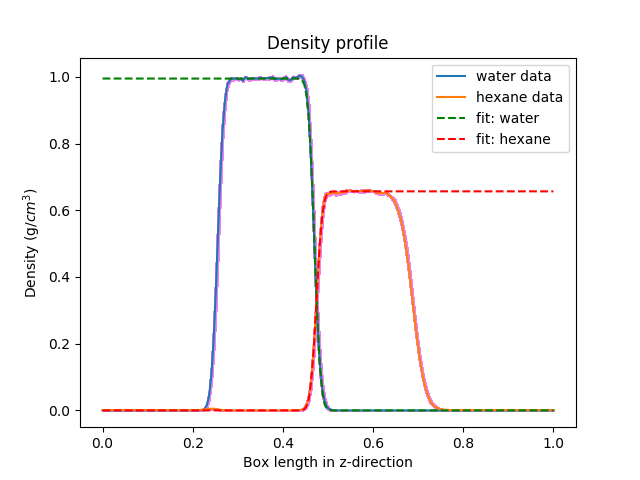
\includegraphics[scale=0.6]{interface_density_profile_individualfit_NVTprod-1bead}
\end{figure}

\begin{figure}[H]
\centering
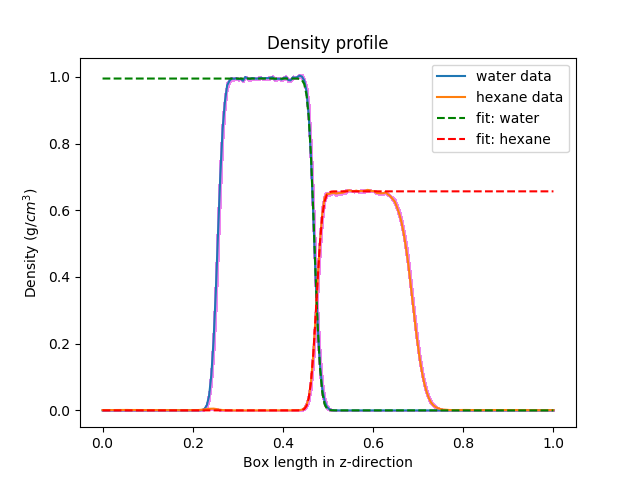
\includegraphics[scale=0.6]{interface_density_profile_simultaneousfit_NVTprod-1bead}
\end{figure}

\begin{figure}[H]
\centering
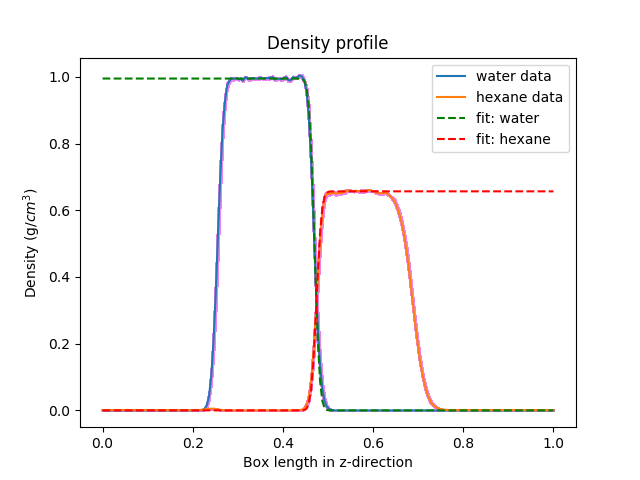
\includegraphics[scale=0.6]{interface_density_profile_blockfit_NVTprod-1bead}
\end{figure}

So, this is interesting.  Everything looks decent.  \\

In fact, the interfacial tension is also reduced, which makes sense with the increased block-averaged thermal width.  The average interfacial tension is 57.2929893303.  

Let's now do the same analysis for the 16 bead and 32 bead versions.

\item Using density\_analysis.sbatch and density\_profile\_postproduction\_PI.py adjusted for 16 beads and the 3,000,000 full NVT data from NVTequil-16bead-long.xyz, we will again perform the postproduction stuff to get densities\_water\_NVTequil-16bead-long.txt etc.  

\item Realized that the 16 bead and 32 bead long simulations did not finish, since their wall time given was only 24 hours.  We really do need 2000 points of production data, though, so I am changing the DASH script to record the trajectory every 1,000 steps instead of 10,000, as well as increasing the wall time on the sbatch script.  These files are waiting to run.  Because there is buildup of stuff on DASH, we will create a new file interface\_new\_NVT32.py that has the 32 beads.  

\end{enumerate}

\section{5/13/2018}

\begin{enumerate}
\item NVTequil-16bead-long finished running, so we are now using density\_analysis.sbatch and density\_profile\_postproduction\_PI.py to create the density profiles for the simulation, after the initial 1 million timesteps of equilibration time.  So, this will give us 2000 (for 2 million production) steps, as we skip over the first 1000.  
\end{enumerate}

\section{5/14/2018}

\begin{enumerate}
\item The above didn't work because it is killed for having too much memory.  We need to read this large file, NVTequil-16-bead-long.xyz, line by line.  So, wrote a python script that does this, called density\_profile\_postproduction\_PI\_largefile.py.  It is intended to skip over the first 1000 recordings of trajectory in order to get to the relevant 2000 production steps.  This is running right now on depablo node.  Before we run 32 bead, let's see if this starts recording density properly.  
\item Created a file density\_profile\_postproduction\_PI\_largefile32.py for the 32 bead version.  Running now.  
\end{enumerate}

\section{5/15/2018}
\begin{enumerate}
\item The 16 bead analysis has gotten through nearly 700,000 steps out of 2 million in nearly 24 hours of running.  So, let's take a look at what we have so far.  We can restart the analysis once this program runs out of time.  But for the time being, let's see. 
\item Downloaded densities\_water\_NVTequil-16bead-long.txt into the interface folder on laptop.  
\item Modifying density\_profile\_analysis.py so that we can use it for multiple beads.  The z box length is the same as in the 1 bead case, i.e. 149.2717.   
\item Based on the 693 samples available, we have:

\begin{align}
\begin{split}
\text{bulk water density: } 0.990280242489 \\
\text{bulk hexane density: } 0.636235151094 \\
\text{separate fitting intrinsic width: } 0.673772951396 \\
\text{water thermal width: } 1.54419798147 \\
\text{hexane thermal width: } 1.47236899979 \\
\text{total intrinsic width: } 0.672263134573 \\
\text{total thermal width: } 1.52334249168 \\
\text{block-averaged intrinsic width: } 0.6770006123 \pm 0.00903193146811\\
\text{block-averaged thermal width: } 1.45879406506 \pm 0.0427265671493 \\
\end{split}
\end{align} 

Here are the individual, simultaneous total, and simultaneous block-averaged plots, respectively: 

\begin{figure}[H]
\centering
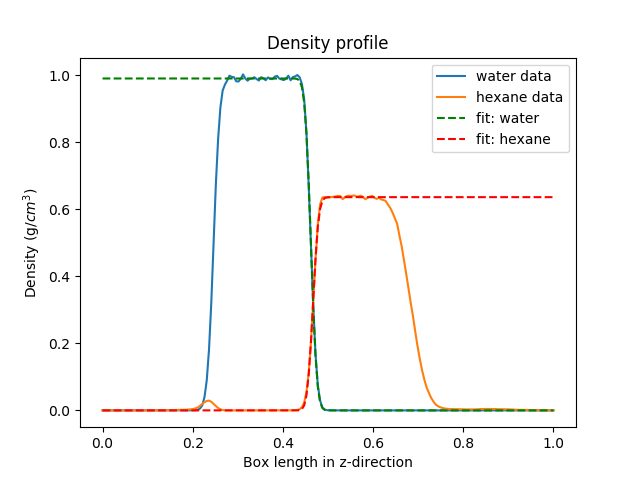
\includegraphics[scale=0.6]{interface_density_profile_individualfit_NVTequil-16bead-long-noSE}
\end{figure}

\begin{figure}[H]
\centering
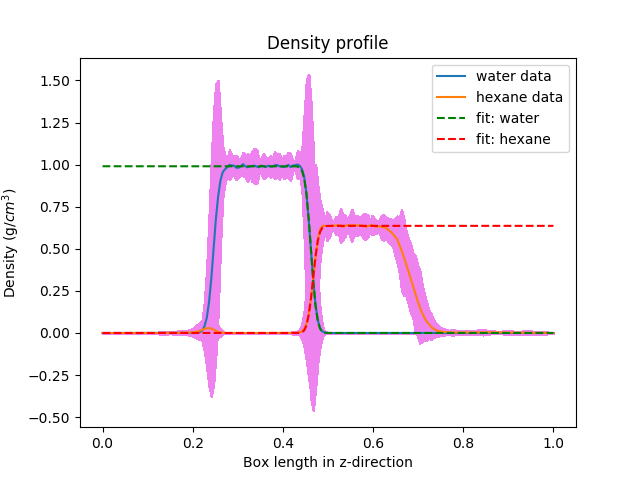
\includegraphics[scale=0.6]{interface_density_profile_individualfit_NVTequil-16bead-long}
\end{figure}

\begin{figure}[H]
\centering
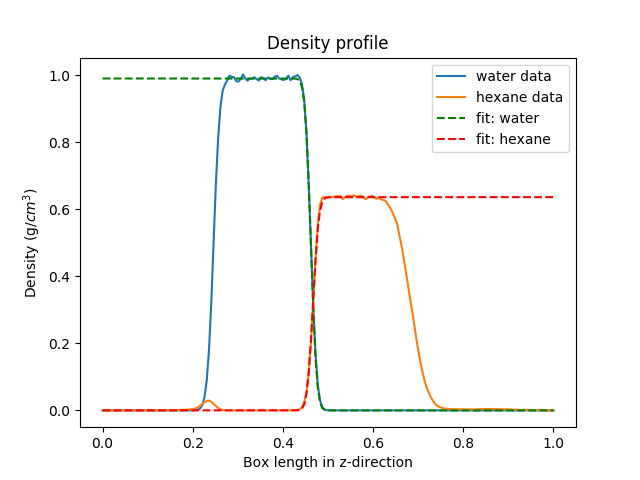
\includegraphics[scale=0.6]{interface_density_profile_simultaneousfit_NVTequil-16bead-long-noSE}
\end{figure}

\begin{figure}[H]
\centering
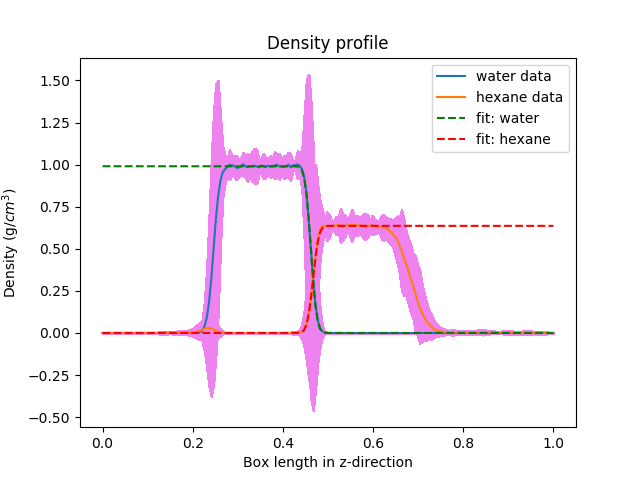
\includegraphics[scale=0.6]{interface_density_profile_simultaneousfit_NVTequil-16bead-long}
\end{figure}

\begin{figure}[H]
\centering
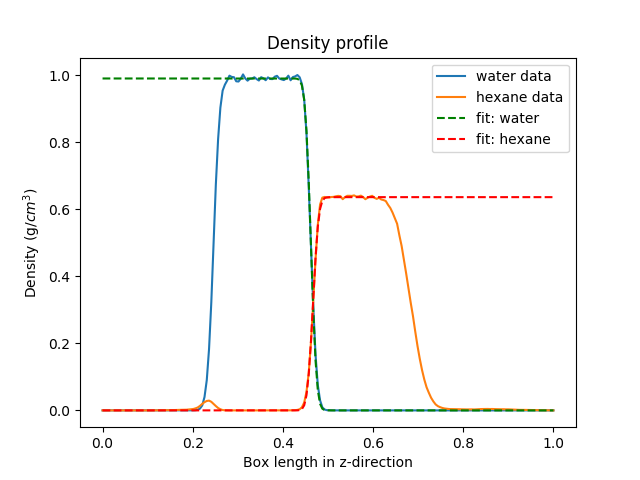
\includegraphics[scale=0.6]{interface_density_profile_blockfit_NVTequil-16bead-long-noSE}
\end{figure}

\begin{figure}[H]
\centering
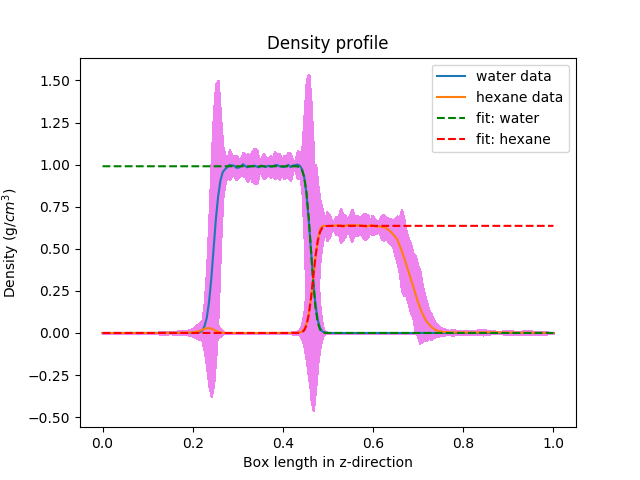
\includegraphics[scale=0.6]{interface_density_profile_blockfit_NVTequil-16bead-long}
\end{figure}

\item Not sure what's going on with the crazy SE or why the total thermal width and block-averaged thermal widths are completely different.  Must have to do with the block size and with the bin size, on both counts. 

\item Here are the results for 32 beads:

\begin{align}
\begin{split}
\text{bulk water density: } 0.990991742448 \\
\text{bulk hexane density: } 0.635954610345 \\
\text{separate fitting intrinsic width: } 0.676349534146 \\
\text{water thermal width: } 1.56571216603 \\
\text{hexane thermal width: } 1.4629537973 \\
\text{total intrinsic width: } 0.67576621799 \\
\text{total thermal width: } 1.53634155284 \\
\text{block-averaged intrinsic width: } 0.685151996303 \pm 0.0153423232413\\
\text{block-averaged thermal width: } 1.50655274353 \pm 0.0731023126283 \\
\end{split}
\end{align} 



Here are the individual, simultaneous total, and simultaneous block-averaged plots, respectively: 

\begin{figure}[H]
\centering
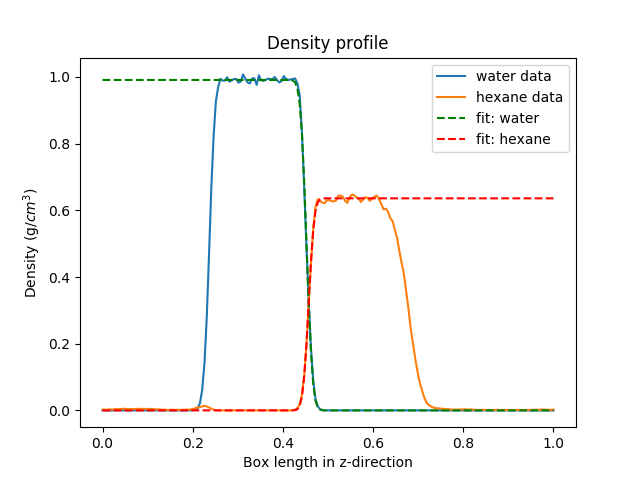
\includegraphics[scale=0.6]{interface_density_profile_individualfit_NVTequil-32bead-long-noSE}
\end{figure}

\begin{figure}[H]
\centering
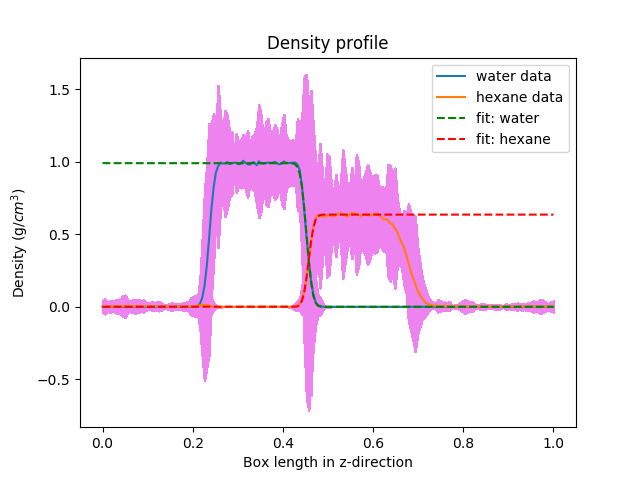
\includegraphics[scale=0.6]{interface_density_profile_individualfit_NVTequil-32bead-long}
\end{figure}

\begin{figure}[H]
\centering
\includegraphics[scale=0.6]{interface_density_profile_simultaneousfit_NVTequil-32bead-long-noSE}
\end{figure}

\begin{figure}[H]
\centering
\includegraphics[scale=0.6]{interface_density_profile_simultaneousfit_NVTequil-32bead-long}
\end{figure}

\begin{figure}[H]
\centering
\includegraphics[scale=0.6]{interface_density_profile_blockfit_NVTequil-32bead-long-noSE}
\end{figure}

\begin{figure}[H]
\centering
\includegraphics[scale=0.6]{interface_density_profile_blockfit_NVTequil-32bead-long}
\end{figure}

\end{enumerate}

\section{5/16/2018}
\begin{enumerate}
\item We failed to record interfacial tension for the 16 and 32 bead examples.  Must incorporate that next time.  
\item First, since we have remaining data sitting there, we should finish collecting all of this data.  The file, densities\_water\_NVTequil-16bead-long.txt has 741 entries.  This means that 
\item Markland group: MD code for path integrals, on graphis cards, OpenMM.  Download this and run it.  See how it compares to what we have.  Compare with 1000 water molecules.  Raman spectra using some of these models.  Once we validate, we want to do this.  
\end{enumerate}

\section{5/21/2018}
\begin{enumerate}
\item First we are going to clean up the code.  
\end{enumerate}

\section{5/25/2018}
\begin{enumerate}
\item To Do:
\subitem RDFs for water and hexane
\subitem Attempt Nose Hoover barostat for density benchmarking under NPT conditions 
\subitem Finish cleaning up existing code
\subitem Modify density profile post production large file so that we use readline instead of readlines, and so that we do the analysis one frame at a time.  For a given frame, save the information in some numpy array and then do the analysis, then move on to the next frame.  If this doens't work, then just split up the traj file and do it in parallel.  
\subitem For the standard error, split into the 5 subtrajectories and plot each of the subtrajectories, to see if the density profile actually moves around.  If so, then we need to normalize/center the bins so that our analysis is ok.  Also, the bin width is on the order of the value of the interfacial profile, so we need more/smaller bins in order to capture this stuff appropriately.  
\subitem Use OpenMM to benchmark our DASH code.  Read Markland papers.
\end{enumerate}

\section{5/27/2018}
\begin{enumerate}
\item We are currently testing density\_profile\_analysis\_UPDATE.py.  We will test its ability using the files densities\_water\_NVTequil-16bead-long.txt and the corresponding hexane one.  
\item We are also investigating the issue with standard error.  We split the data into two segments for the SE calculation, so that we have means\_water[0] and means\_water[1].  We first find that the SE calculation has not been normalizing number of beads.  So, we do that.  Then, we notice that there is a shift by one bin in the location of the profile.  We print out, for means 0 and means 1, the value of the mean for each of the 200 bins side by side.  
\begin{figure}[H]
\centering
\includegraphics[scale=0.6]{interface_density_binshift}
\end{figure}
\item Nevertheless, even with this slight shift, we find that normalizing for beads fixes the SE problem.  
\begin{figure}[H]
\centering
\includegraphics[scale=0.6]{interface_density_profile_beadnorm}
\end{figure}
\item Now, we will create density\_profile\_postproduction\_PI\_largefile\_UPDATE.py to analyze NVTprod-1bead.xyz as a test.  
\end{enumerate}

\section{5/28/2018}
\begin{enumerate}
\item We have created density\_profile\_postproduction\_PI\_largefile\_UPDATE.py and began to analyze NVTprod-1bead.xyz successfully.  However, we should make sure we can do a complete file successfully, and we don't want to wait for this one to finish.  So, let's create some test trajectory files, with 1, 16, and 32 beads, and 10 frames, to check that the analysis is done appropriately.  
\item Significantly sped up system by using the readline() format and by using np.digitize() for the histogram computation.
\item Now, we will use this program to analyze NVTequil-16bead-long.xyz, hopefully getting the FULL trajectory this time!  Uploaded density\_profile\_postproduction\_PI\_largefile\_UPDATE.py to midway.
\item Seems to work on Midway.  So, we are going to do the following.  We will use this script to collect density profiles from NVTequil-16bead-long.xyz and NVTequil-32bead-long.xyz.  The density text files will have the file name NVTequil-16bead-long-FULL, and the same for 32 beads.  We run these from density\_analysis.sbatch.    
\item Something else we want to check is what happens when we increase the number of bins from 200.  Because we want our error to be small enough relative to the intrinsic width. So, perhaps we want an order of magnitude larger number of bins.  
\end{enumerate}

\section{6/1/2018}
\begin{enumerate}
\item Full collection of density profiles took less than 24 hours, so we now have completed files densities\_water\_NVTequil-16bead-long-FULL.txt and densities\_hexane\_NVTequil-16bead-long-FULL.txt.  We will first download these onto laptop.  
\item Now we will use density\_profile\_analysis\_UPDATE.py to analyze these profiles, taking care to remove the first ns of profile data, which is the equilibration period.  The z box length is the same as before, 149.2717.  So, we use the second two ns of data, from indix 1000 to 3000.  The analysis reveals the following: 

\begin{align}
\begin{split}
\text{bulk water density: } 0.995624283643 \\
\text{bulk hexane density: } 0.638737730535 \\
\text{separate fitting intrinsic width: } 0.646069228603 \\
\text{water thermal width: } 1.6887345795 \\
\text{hexane thermal width: } 1.62750350738 \\
\text{total intrinsic width: } 0.645278775844 \\
\text{total thermal width: } 1.67098576921 \\
\text{block-averaged intrinsic width: } 0.657563761558 \pm 0.0175256170729\\
\text{block-averaged thermal width: } 1.56668743686 \pm 0.0300388678349 \\
\end{split}
\end{align} 

Here is a plot using the block-averaged fitting parameters:

\begin{figure}[H]
\centering
\includegraphics[scale=0.6]{interface_density_profile_NVTequil-16bead-long-FULL}
\end{figure}

\item For the same thing above but with 32 beads, we obtain:

\begin{align}
\begin{split}
\text{bulk water density: } 0.997054790967 \\
\text{bulk hexane density: } 0.632792582469 \\
\text{separate fitting intrinsic width: } 0.610323859405 \\
\text{water thermal width: } 1.75865687055 \\
\text{hexane thermal width: } 1.67544835215 \\
\text{total intrinsic width: } 0.608799880016 \\
\text{total thermal width: } 1.73427604532 \\
\text{block-averaged intrinsic width: } 0.626126706412 \pm 0.0217244653966\\
\text{block-averaged thermal width: } 1.5643927083 \pm 0.0310262340524 \\
\end{split}
\end{align} 

\begin{figure}[H]
\centering
\includegraphics[scale=0.6]{interface_density_profile_NVTequil-32bead-long-FULL}
\end{figure}


\end{enumerate}

\section{6/4/2018}
\begin{enumerate}
\item Looking at Mike's folder, for\_kirk\_rdf, in order to compute the RDF for TIP4P/F water.  
\item Not sure how to use this file, so waiting for Mike to come in to deal with this.  Hopefully we can fully validate our implementation of TIP4P/F within a day or two.  
\item For the time being, moving on to computing density profiles using a larger number of histogram bins.  We will first try 2000.  Modified density\_profile\_postproduction\_PI\_largefile\_UPDATE.py to allow for easy modifications of number of bins.  Let's now run this for our current NVTequil-16bead-long.xyz and NVTequil-32bead-long.xyz files.  The density text files will be named NVTequil-16bead-long-2000bins and NVTequil-32bead-long-2000bins, respectively.  Again, we will run these from density\_analysis.sbatch.  These are both running now.  
\item We have not yet analyzed molecular orientation at the interface for NVTequil-16bead-long.xyz or NVTequil-32bead-long.xyz.  The python scripts that perform this analysis, molecular\_orientation\_postproduction.py and molecular\_orientation\_postproduction\_hexane.py, rely on the old way of loading .xyz files, which is not suitable for large files.  So, we are going to have to rewrite these scripts to make them suitable for large files, in a similar vein as density\_profile\_postproduction\_PI\_largefile\_UPDATE.py.  Also, we have to adapt this for multiple beads...
\item For the time being, though, we will work with interface-dens.xyz, which according to notes from 4/17/2018: "It appears to be working.  Modified the original interface.py to reflect this, as well as customizing filename for the density files.  Currently running DASH simulation of the interface using 400,000 preequilibration steps, followed by 300,000 production steps during which density profiles are measured every 100 steps."  It appears as though there are about 620 frames in this file, and that the system equilibrates after 300,000 steps.  So, we will assume we have 300,000 equilibration and 200,000 production NPT steps using 1 bead.  
\item Liu heavy light water notes orientation needs to be done on a per bead basis, and also that there are non substantial (but measurable?) quantum effects to interfacial H-bond network.
\item Wrote a file, molecular\_orientation\_water\_postproduction\_UPDATE.py, which improves the file reading process as noted above.  We are going to test this on interface-dens.xyz on Midway.  If this works, we will make similar changes to allow for hexane profile analysis, and then test this for 16 beads.   Running this now using orientation\_postproduction.sbatch.  
\item The resulting filename is orientations\_water\_interface-dens-test.xyz.  Bringing this now to laptop.  
\item The result, tested using orientation\_profile\_analysis.py, appears to work.  So, let's now move on to the 16 bead case.  So we will us the traj file NVTequil-16bead-long.xyz.  We will call the orientation file NVTequil-16bead-long-orientations.   
\item We will run the same thing for 32 beads, with a similar file name.  
\item Talked to Mike about RDF stuff.  I think we have a clear read on what to do.  The first thing to do is to take the 1 bead water output file, say kirk\_tip4p\_1950000.xml and move that data into a LAMMPS file containing the relevant bond, angle, and dihedral information.  
\item Went to lammps\_work/water on laptop and used the molecule replicator to create a file, RDF.sys.data, which I then moved to dash\_work/water.  Modified the header to have the right format of atoms, atom types, bonds, bond types, etc., and showing zero dihedrals. Working on a python script called dash\_restart\_to\_lammps\_RDF.py.    
\end{enumerate}

\section{6/5/2018}
\begin{enumerate}
\item For RDFs, in for\_kirk\_rdf/RDF.  ./comp\_mod cmd\_read\_subs.  then, , ./compile.sh.  
\item MUST include total number of atoms in data file, including M site.  Finished script dash\_restart\_to\_lammps\_RDF.py.  Used this in conjunction with a 2M fs NPT output, output\_dens.xyz, to construct RDF using ./get\_rdfs 1 output\_dens.xyz RDF.tip4pF.data.txt < example\_rdf.input.  Resulting file 0\_0.rdf was analyzed in new python script in the dash\_work/water folder on laptop, called RDF\_analysis.py, which produced the following plot:
\begin{figure}[H]
\centering
\includegraphics[scale=0.6]{RDF}
\end{figure}
\end{enumerate}

\section{6/6/2018}
\begin{enumerate}
\item Wrote python script tip4pF\_UPDATE in dash\_work/water.  Using this to do validation of TIP4P/F in DASH.  
\item From Markland paper: "For example, the O-O, O-H, and H-H RDFs of the two liquids were obtained from 250 ps NVT path integral simulations in the presence of an Andersen thermostat."
\item "...and liquid densities at 1 atm pressure were obtained from 10 ns NPT simulations in order to fully converge the average over density fluctuations.  These latter simulations were performed in the presence of both an Andersen thermostat and an isotropic Berendsen barostat."  
\item "Unless stated otherwise, all of our liquid simulations were performed at a temperature of 298K and a density of 0.997 g/cm3 with 216 water molecules in a cubic simulation box...Short-range interactions were truncated at 9 A...Thirty-two ring polymber beads were used in all simulations..Several classical simulations were also performed for comparison by collapsing the ring polymer to a single bead (n = 1)."
\item "In all simulations, the system was equilibrated for 100 ps in the presence of an Andersen thermostat before the accumulation of any averages."    
\end{enumerate}

\section{6/7/2018}
\begin{enumerate}
\item First, let's set up simulations to construct RDF plots similar to Markland.  They did 100 ps NVT equilibration followed by 250 ps NVT production with 216 molecules at a density of 0.997 g/cm3 and 32 beads and at a temperature of 298K.  Short range cutoff at 9 Angstroms.  
\item So, we will do 200,000 steps of equilibration followed by 500,000 steps of production, with 216 molecules, density of 0.997, temperature of 298.0K, short range cutoff at 9 Angstroms, and 32 beads.  Because we simply want to record the trajectories, we will only record the .xyz during production run, and we will record at a frequency of every 100 steps, which should give us 5000 frames for analysis.  General data is also recorded every 100 steps.  
\item For 1 bead, the filename is RDF-1bead.  For 32 beads, the filename is RDF-32bead.  
\item These finished running within the hour.  Next, we will extract the RDF information.  
\item Copied .xyz files to for\_kirk\_rdf/RDF/tip4pF.  Also copied data\_water\_flexible.txt and lammps\_molecule\_replicator\_water.py from hexane-water/lammps\_work/water.  Went into the replicator file and set the number of molecules to 216.  Creating an output file called RDF-tip4pF.data.  
\item Ran a very brief simulation to extract a dash restart file for 216 water molecules, file called RDF-restart0.xml.  Also brought in dash\_restart\_to\_lammps\_RDF.py.  Had to make changes to this file, because it was written using old dash restart files rather than NEW\_DASH.    
\item Used this to create an artificial lammps file, sys.RDF-tip4pF.data.txt.  Manually rearranging the header so that we include M site in the count and that atoms, atom types, bonds, bond types etc. is the order.  
\item To run get\_rdfs, must first module load gcc/4.9.  
\item Saving the rdf data on laptop in hexane-water/data folder as 0\_0-1bead-tip4pF.rdf etc.  
\item Here are the results for 1 bead:

\begin{figure}[H]
\centering
\includegraphics[scale=0.6]{0_0-1bead-tip4pF.png}
\end{figure}

\begin{figure}[H]
\centering
\includegraphics[scale=0.6]{0_1-1bead-tip4pF.png}
\end{figure}

\begin{figure}[H]
\centering
\includegraphics[scale=0.6]{1_1-1bead-tip4pF.png}
\end{figure}

\item Downloading densities\_water\_NVTequil-16bead-long-2000bins.txt and the hexane equivalent to laptop.
\item The 32 bead RDF did not work.  We need to include total number of atoms, with the discretization, in the lammps data file that we artificially create.  So, creating a new .xml output with 32 beads.  We also have to manually adjust the header, in addition to what we did before, by multiplying the atom number, bond, number, and angle number by 32, the number of beads.  


\end{enumerate}

\section{6/10/2018}
\begin{enumerate}
\item Now, we have the 32 bead info, which we have saved as 0\_0-32bead.rdf etc.  Here are the results for 32 beads, along with the Markland paper plots:

\begin{figure}[H]
\centering
\includegraphics[scale=0.6]{0_0-32bead-tip4pF.png}
\end{figure}

\begin{figure}[H]
\centering
\includegraphics[scale=0.6]{Markland-0_0-RDF}
\end{figure}

\begin{figure}[H]
\centering
\includegraphics[scale=0.6]{0_1-32bead-tip4pF.png}
\end{figure}

\begin{figure}[H]
\centering
\includegraphics[scale=0.6]{Markland-0_1-RDF}
\end{figure}

\begin{figure}[H]
\centering
\includegraphics[scale=0.6]{1_1-32bead-tip4pF.png}
\end{figure}

\begin{figure}[H]
\centering
\includegraphics[scale=0.6]{Markland-1_1-RDF}
\end{figure}

\item We notice that the Markland RDF plots contain bonded species, so we will re-do O-H and H-H RDFs to include bonded and angle species.  
\item This is running now, using run.sh on Midway 1 bigmem.    
\item In Patel and Brooks, density values are likewise obtained for bulk NPT simulations, similar to Markland.  Patel and Brooks also say that their bulk densities are "obtained" from fits to the individual density profiles."  
\item How do we know NVT ensemble is appropriate?  How do we know we are incorporating appropriate conditions?  How do we know densities are appropriate??
\item If we do an NVT simulation but cannot specify an average pressure or pressure range, then how can we compare to experimental measurements of something like interfacial tension or width?  These experiments are naturally carried out at a fixed temperature and at atmospheric pressure.  But what if our NVT simulation has an average pressure that is much greater, or less than, atmospheric pressure?  How can we know to compare our results to what is effectively an NPVT system?  For example, what does density even mean in an NVT context?  I could increase V extremely large but we would still have the same density of the bulk in our simulation.  So how do we compare this experimentally?  I guess it would mean something if we KNEW what the density was.  How do I know that the density of an NVT system with too much room will equilibrate to the density at the same T and at atmospheric pressure?
\item NICOLAS 2004 HEXANEWATER DESCRIBES DEPLETION THING  
\item For 16 beads from NVTequil-16bead-long, and files densities\_water\_NVTequil-16bead-long-2000bins, we have:


\begin{align}
\begin{split}
\text{bulk water density: } 0.991059863363 \\
\text{bulk hexane density: } 0.63864891231 \\
\text{separate fitting intrinsic width: } 0.659180420853 \\
\text{water thermal width: } 1.67546058832 \\
\text{hexane thermal width: } 1.62587346184 \\
\text{total intrinsic width: } 0.658660739701 \\
\text{total thermal width: } 1.66111444442 \\
\text{block-averaged intrinsic width: } 0.670463724935  +/- 0.0164082418884\\
\text{block-averaged thermal width: } 1.55491430753  +/- 0.0298681614987 \\
\end{split}
\end{align} 

\end{enumerate}

\section{6/11/2018}
\begin{enumerate}
\item Downloading the new RDFs that include bonded species.
\item Plotting them:

\begin{figure}[H]
\centering
\includegraphics[scale=0.6]{0_1-32bead-bonded-tip4pF.png}
\end{figure}

\begin{figure}[H]
\centering
\includegraphics[scale=0.6]{0_1-32bead-bonded-tip4pF_1.png}
\end{figure}

\begin{figure}[H]
\centering
\includegraphics[scale=0.6]{0_1-32bead-bonded-tip4pF_2.png}
\end{figure}

\begin{figure}[H]
\centering
\includegraphics[scale=0.6]{1_1-32bead-bonded-tip4pF.png}
\end{figure}

\item Updated plot for O-O 32 bead: 

\begin{figure}[H]
\centering
\includegraphics[scale=0.6]{0_0-32bead_2.png}
\end{figure}

\item Nick says that temperatures can be lowered to like 200 K for a water model.  So, I will just check myself.  

\end{enumerate}

\section{6/12/2018}
\begin{enumerate}
\item First, let's make sure water is completely finished.  We will start by organizing the water folder, removing unnecessary elements, updating the GitHub, and then recomputing the TIP4P/F RDFs using a finer bin size.  
\end{enumerate}

\section{6/13/2018}
\begin{enumerate}
\item Taking from 6/7/2018, we will again analyze the results from RDF-32bead-freq100.xyz to construct the appropriate RDFs, but with a finer bin size.  Running the O-O using bin size of 0.05 instead of 0.1 as a test.  If this works, we will compute the others.  
\item The problem is that this no longer works on bigmem.  It works on the local node, but not on the depablo node.  So, we are going to have to diagnose what the issue is.  It might be a problem with memory usage in the RDF code.  Finalizing the RDFs will have to wait.  
\item In order to get accurate measurements of the pure TIP4P/F density, we will run 216 molecules at 1.0 atm, classical, doing 100 ps (200,000 steps) of equilibration followed by 10 ns (20,000,000 steps) of production.  Filename is density\_calc followed by temperature.  We will check 250, 270, 275, 285, 298, 320, 340, 360.  We are starting by running T = 298.  
\end{enumerate}

\section{6/14/2018}
\begin{enumerate}
\item Tried running water using the new python script tip4p.py, but it failed after 3,690,900 steps.  The error given was: 
\begin{figure}[H]
\centering
\includegraphics[scale=0.6]{water_error}
\end{figure}
\item Let's try running the old script from GitHub (which is basically just taken from Mike).  We will figure this out.  Perhaps it has to do with data collection or how I've written the new script.  It shouldn't fail after less than 4 million steps.  
\item Well, despite these issues, we at least know that the interface should be working.  So, let's just look at that for now.   
\item We will do fully NVT simulations using 1 bead and fully NVT simulations using 32 beads.  For each we will equilibrate the system for 1 ns and then do production for another 3 ns.  We will collect trajectories every 1000 steps and record restart files every 500,000 steps.  We will test temperatures 298, 285, 275, 270, 250, and 235.    Filename is full-1bead-298 for 298 K.  Actually, after 1 bead 298, we are going to switch this to full-<temperature>-1bead.  
\item This time the tip4pF.py file failed after only 2236500 steps.  Changing the barostat to have a parameter of 10000 instead of 1000.  Changed temperature to 298.15 instead of 298.  Made change so that production xyz's are recorded at trajFreq1 and trajFreq2 instead of accidentally hard-coded 100 and 50.  
\item Was able to run the RDF program on depablo-gpu without specifying gres=gpu:1.  Running this now trying bin size of 0.01.  Set the time limit to 72hr in case it takes longer.  
\end{enumerate}

\section{6/15/2018}
\begin{enumerate}
\item For water, we will test densities 235, 250, 270, 275, 285, 298, 320, 340, 360 as described above.  
\end{enumerate}

\section{6/19/2018}
\begin{enumerate}
\item Currently retrieving the densities for pure water 1 bead as described above.  235 complete, 250 complete, 270 complete, 275 complete, 285 complete, 298 complete, 320 complete, 340 complete, 360 complete.  
\item Ok, now that we have this data, we want to rigorously compute average density values and corresponding uncertainty estimates using the standard error.
\item The standard error is simply the standard deviation of the sampling distribution of the mean.  The sampling distribution is when you pick $n$ items from a population, add them together, and then divide the sum by $n$.  To get the standard deviation of this quantity, we get the variance and take the square root.  So, we have 

\begin{align}
\begin{split}
\text{Var}\left(\frac{\sum_{i=1}^nX_i}{n}\right) = \frac{1}{n^2}\text{Var}\left(\sum_{i=1}^nX_i\right) = \frac{1}{n^2}n\sigma^2 = \frac{\sigma^2}{n}
\end{split}
\end{align} 
We then take the square root to get the standard error $\frac{\sigma}{\sqrt{n}}$.  (https://stats.stackexchange.com/questions/89154/general-method-for-deriving-the-standard-error).  $\sigma$ is the standard deviation of the population. When the standard deviation of the population is not known, we can use the sampling standard deviation $s$.  
\item To get statistically rigorous estimate of the average values and errors in a simulation. we do block averaging.  As explained in https://www.ncbi.nlm.nih.gov/pmc/articles/PMC2865156/, a trajectory with $N = M\cdot n$ snapshots is divided into $M$ blocks with an initial very short block length, such as $n = 1$.  The average of an observable is calculated for each block yielding $M$ values.  The block length $n$ is gradually increased and the set of block averages is recalculated for each length.  Further, for each value of $n$, the standard deviation among the block averages, $\sigma_n$, is used to calculate a running estimate of the overall standard error, namely $\frac{\sigma_n}{\sqrt{M}}$, which is the standard error in estimates of the mean based on blocks of length $n$.  This value increases monotonically with $n$ and asymptotes to the true standard error associated with the average observable value.  
\item So, let's create a python script density\_analysis.py and apply the block averaging technique to analyze density for 216 TIP4P/F molecules, 10 ns of production, 1 bead, in the file.
\item Well, the bad news is that the simulations I ran were NVT.  Crap.  So, we are going to have to re-do this.  Man, it is pretty ridiculous how long this is taking me.  Let's get a move on already. 
\item Now re-running the water densities in NPT conditions.   
\item Going in to /project/depablo/kswanson/hexane-water/dash\_work/water/RDF-new/tip4pF to get the RDF we computed on 32 bead trajectory, 216 molecules, NVT for 200 ps as described earlier.  This time, we used a bin size of 0.05 instead of 0.1 to see if the RDFs get any smoother.  We will download these rdfs into laptop and then print images. 
\item If densities fail, we will have to either analyze the xyz trajectory or periodically write out the densities using a python operation.  Alternatively, we could just manually run 2 at a time and collect densities over time.    
\item As an update to the RDFs, we computed the same as before using the full 32 bead trajectory, except this time we used a bin size of 0.05 instead of 0.1:

\begin{figure}[H]
\centering
\includegraphics[scale=0.6]{0_0-32bead-bonded-tip4pF-bin05.png}
\end{figure}

\begin{figure}[H]
\centering
\includegraphics[scale=0.6]{0_1-32bead-bonded-tip4pF-bin05.png}
\end{figure}

\begin{figure}[H]
\centering
\includegraphics[scale=0.6]{1_1-32bead-bonded-tip4pF-bin05.png}
\end{figure}

\item To get slightly sharper images, we will try a bin size of 0.01, and then just call it quits after that.  We will do this in the folder RDF-new/tip4pF.  
\item Now we are going to do full analyses of the interfacial 1 bead and 32 bead cases.  
\item First, we will analyze filenames full-1bead-298, which consist of 500 ps (1,000,000 steps) of equilibration and 1.5 ns (3,000,000 steps) of production, both in the NVT ensemble, using 1 bead, restart files catalogued every 500,000 steps, trajectory recorded every 1,000 steps, ptensor recorded every 20 steps, waldman mixing.  So, first, we will look at interfacial width measurements.  Using density\_analysis.sbatch, which runs density\_profile\_postproduction\_PI\_largefile\_UPDATE.py, we collect the density profiles at each trajectory step using 2000 bins and 20000 bins.  The resulting text files are labelled like densities\_water\_full-1bead-298-2000bins-density\_profiles.txt (or 20000).  
\item We will then download these files and apply density\_profile\_analysis\_UPDATE.py.  
\item Realized that I did not expand the box size for these simulations.  damn.  So, we are going to have to re-do all of them.  
\item These are running now.
\item Another thing for pure water density to test is if the restart begins whether or not the .xyz file will simply be added to or if a new file is created.  Hopefully it will simply be added to, because then when we restart the xyz file will be continuously added to and we can simply do the density analysis using the bounds and mass information from the .xyz file.  or print out the mass before the simulation or something. 

\end{enumerate}

\section{6/21/2018}
\begin{enumerate}
\item We will begin today by analyzing the set of 1bead NVT interface runs, which consist of: 500 ps (1M steps) NVT equilibration, 3 ns (6 M steps) production, where the volume was extended by 20 on both sides, 1 path integral bead, restart files every 1M steps, traj recorded every 1000 steps.  We will start as above by using density\_analysis.sbatch, which runs density\_profile\_postproduction\_PI\_largefile\_UPDATE.py, we collect the density profiles at each trajectory step using 2000 bins.  The resulting text files are labelled like densities\_water\_full-1bead-298-2000bins.txt.  
\item Now downloading these text files to laptop.  We will now use density\_profile\_analysis\_UPDATE.py.  
\item We are choosing to analyze the last 6000 frames, which correspond to the production data, so we choose index\_start=1001 and index\_end=7001.  
\item Updated density\_profile\_analysis\_UPDATE.py to include block averaging analysis.  Here are the results:

\begin{figure}[H]
\centering
\includegraphics[scale=0.6]{density_profile_block_averaging_1_full-298-1bead}
\end{figure}

\begin{figure}[H]
\centering
\includegraphics[scale=0.6]{density_profile_block_averaging_2_full-298-1bead}
\end{figure}

Using 200 ps blocks, which is in line with the literature, appears to be a reasonable choice for size when calculating averages and standard errors.  

\item So, on 6M steps of production data (3ns), using 15 blocks of size 200 ps, z length 149.2717, 2000 bins, bulk water between 600 and 800 indices (or 44.78151 Angstroms and 59.70868), bulk hexane between 1100 and 1240 indices (or 82.099435 and 92.548454 Angstroms), we have from simultaneous fitting (and the bulk regions):

\begin{align}
\begin{split}
\text{bulk water density: } 0.995713529553  +/- 0.000227886323623 \\
\text{bulk hexane density: } 0.656683170779  +/- 0.000744213918941 \\
\text{block-averaged intrinsic width: } 0.649073945814  +/- 0.00577251469653\\
\text{block-averaged thermal width: } 1.48440988479  +/- 0.0186896325302 \\
\end{split}
\end{align} 

\item Working on tension\_analysis\_UPDATE.py.  Downloading the pressure tensor info from full-298-1bead, pressure\_tensors-full-198-1bead.txt.  

\item How can Patel cite an appropriate interfacial tension compared to experiment given NVT?

\item Interfacial tension overall is 37.9, but the SE is like 400.  What the fuck is going on?  How does this compare to an equivalent NPT simulation?  To check this, we are running full-298-NPT, which is the same as full-298-1bead but with NPT conditions (no PI), and no z-expansion of the box.  
\item Also try collecting this information every half femptosecond so we have more data, and also DO NOT DIVIDE BY 1/2 BECAUSE WE NO LONGER HAVE TWO INTERFACES, and also try doing the simulation NVT with no additional volume added so that it is just like Patel and also look at other temperatures to see how they are comparatively.  Perhaps just collect a huge amount of data?

\end{enumerate}

\section{6/25/2018}
\begin{enumerate}
\item Current To Do List:
\subitem Reading on geochemical isotope fractionation motivation for the hexane-water problem
\subitem Make RDF calculator compatible on depablo node by using multiple processors (-ntasks-per-node, can even specify amount of memory to use)
\subitem Look at Mike's Anisotropic MC Barostat, test it, see what is wrong, and try to fix it.  
\subitem When using the NVT with expanded boundaries, find a way to calculate the pressure of the total system (if it doesn't change too much from 1 atm we are fine).  Perhaps use the Elastic bath method.  
\subitem Read about pure water/vapor interface, and look up path integral papers by Paizani (use this as motivating context)
\subitem Compute primary pure water/vapor interface properties 
\subitem Fix pressure calculation in PIMD code, and add capability to compute pressure tensor elements (or interfacial tension) across a specified box length 
\subitem Read Tuckerman wodrk/virial theorem, and section 12.3.  
\subitem Consider simulating W-H-W interface with vapor on both sides
\subitem Consider simulating the NVT extra volume as we have been doing, but then remove the vacuum and choose the average "box" size containing the molecules in order to simulate at NVT with no extra space, thus allowing us to do the interfacial tension calculation once the pressure aspect has been fixed in PIMD? 
\subitem Compare DASH results to OpenMM
\subitem Finish computing interfacial width measurements from multiple temperatures using 1 and 32 beads. 
\subitem TAFFI hexane - has it really been parametrized for 32 beads?  Density is correct at 1 bead so... 
\subitem For interfacial tension, collect every single half femtosecond to get more data?  And also simulate longer?  Choose better block sizes?
\subitem Fix interface\_UPDATE.py so that pressure tensor information is output at regular intervals, so that if a restart is needed we don't lose all of that information.  
\subitem Check full-298-NPT run to see if pressure tensor calculations are any more stable.  Consider running a Patel-style NVT run also to check this.  
\subitem Compute the 90-10 width for comparison.  
\subitem Optimize TAFFI hexane for 32 beads.  Density as a function of epsilon and sigma. 
\subitem Hexane orientation for 32 beads.   
\subitem Compute density profiles using 20,000 bins
\subitem Check out what's going on with the 32 versus 1 bead molecular orientations - is this a coding error?  If not, how does this line up with experimental information, and how does it compare to the previous story of a "double" layer in other simulation papers?  
\subitem Mike D2O paper, geology ideas, Paizani, https://pubs.acs.org/doi/abs/10.1021/ct5004115, https://pubs.acs.org/doi/pdfplus/10.1021/acs.jpclett.7b00979
\subitem Clean up code generally 
\subitem DON'T FORGET that I made special changes to utils.py, specifically the water stuff, for restart as opposed to random in create tip4p flexible.  
\subitem Fix pure water (and hexane) DASH code with appropriate restart protocols (similar to fixes for interface code)
\subitem Read Markland papers, and ion stuff?  solid water interfaces?
\subitem Patel says that bulk densities were obtained from fits to the individual liquid density profiles...we could try that
\subitem Whey are there ANY values of water orientation, say, inside the hexane region??
\subitem URGENT: Confirm that pure TIP4P/F water with 1 bead and 32 beads has a non-ice RDF.  Also confirm this for TAFFI hexane.  Make it clear on the data table slide that Patel and Brooks implemented a different model.  Put simulation values on slide 16 for densities, as well as experimental.  Compute 1 bead MC Barostat density, check 8, 16, 32 beads, to see what is going on here.  Do a brute force pressure calculation to find pressure of the NVT systems (can only do this for 1 bead) to check what pressure we are computing values at.  Characterize everything in NPT to show full proof of concept.  Run at more temperatures to see that the difference in intrinsic widths does not jump at 250.  UNDERSTAND why computing the pressure is important?  Understand why we can't compute pressure currently with PIMD.  Use OPLS/LAMMPS to compute the RDF for hexane, and use THAT to compare to TAFFI hexane and also show that low temperature hexane is fine.  Do the NVT system using a restricted V, compute pressure, then expand V (32 beads) until we get P = 1.0 atm....brute force way of achieving the appropriate density of the system without extra vacuum.  

\item Today, we will start by checking the 32 bead calculations at a variety of temperatures to see if they finished running.  They did not finish running, only got about 60\% through the production run.  So, we should try to do a restart of these simulations using their last saved restart file.  We may have to add restart capability to the file used to simulate these runs, interface\_UPDATE.py.  We will also check that the simulation will simply continue to add to the already-existant .xyz file, so that we don't lose information. 
\item .xyz files when restarted are overwritten, not added to.  So, we will have to do a separate xyz file and then combine them.  We will use the command cat a.txt b.txt > c.txt
\item We have also realized that in order to avoid the problem of overlapping .xyz files after a restart, we need to have the restart file and trajectory files recorded at the same frequency.  And because of this, we need to not record a separate .xml file every 1000 steps since that would be ludicrous.  So, we will change interface\_UPDATE.py to not only avoid writing the initial config during restart, but also to generally avoid writing separate .xml files.  It's not like I've ever needed that anyway.  
\item DASH writes files at step 1001 if the freq is set to 1000.  So, need to set number of steps to 1001 if want to capture the 1000th configuration I think.  OR, just have the system writeConfig at the end of the simulation.  Then, when we restart, we will just have a double configuration in the trajectory file. 
\item Implemented these changes. 
\item Running the 32 bead, NVT, 1M equil, 6M prod, write freq 1000, tensor freq 20, expanded box size by 20 angstroms.  
\item Now we are going to finish analyzing the rest of the 1 bead data as before.  
\item We first use density\_analysis.sbatch to collect density profiles with 2000 bins.  We are doing this for temperatures 235, 250, 270, 275, 285.  
\item Now we will download these files to laptop.   
\item Block-averaging analysis for temperature 285:
\begin{figure}[H]
\centering
\includegraphics[scale=0.6]{density_profile_block_averaging_1_full-285-1bead}
\end{figure}

\begin{figure}[H]
\centering
\includegraphics[scale=0.6]{density_profile_block_averaging_2_full-285-1bead}
\end{figure}

Using 200 ps again, i.e. 15 blocks, and the same other parameters as above, we get for 285:

\begin{align}
\begin{split}
\text{bulk water density: } 0.997755320581  +/- 0.000285565797713 \\
\text{bulk hexane density: } 0.671907619392  +/- 0.000559434913252 \\
\text{block-averaged intrinsic width: } 0.583875387151  +/- 0.00638389740959\\
\text{block-averaged thermal width: } 1.43708505118  +/- 0.0220312686935 \\
\end{split}
\end{align} 

\item Block averaging analysis for temperature 275:

\begin{figure}[H]
\centering
\includegraphics[scale=0.6]{density_profile_block_averaging_1_full-275-1bead}
\end{figure}

\begin{figure}[H]
\centering
\includegraphics[scale=0.6]{density_profile_block_averaging_2_full-275-1bead}
\end{figure}

Based on these images we will use 200 ps, i.e. 15 blocks, and the same as other parameters, so we get for 275:

\begin{align}
\begin{split}
\text{bulk water density: } 0.996016559218  +/- 0.0010609755986 \\
\text{bulk hexane density: } 0.684747557408  +/- 0.000617622666816 \\
\text{block-averaged intrinsic width: } 0.52819126805  +/- 0.00957973357639\\
\text{block-averaged thermal width: } 1.41593938545  +/- 0.0388654184264 \\
\end{split}
\end{align} 

\item For temperature 270:

\begin{figure}[H]
\centering
\includegraphics[scale=0.6]{density_profile_block_averaging_1_full-270-1bead}
\end{figure}

\begin{figure}[H]
\centering
\includegraphics[scale=0.6]{density_profile_block_averaging_2_full-270-1bead}
\end{figure}

\item Again using 15 200 ps blocks, we have for 270 K:

\begin{align}
\begin{split}
\text{bulk water density: } 0.998561389514  +/- 0.000314906166251 \\
\text{bulk hexane density: } 0.69042758613  +/- 0.0004139396481 \\
\text{block-averaged intrinsic width: } 0.509291861116  +/- 0.00776010775438\\
\text{block-averaged thermal width: } 1.4160674967  +/- 0.0369387679761 \\
\end{split}
\end{align} 

\item For 250 K: 


\begin{figure}[H]
\centering
\includegraphics[scale=0.6]{density_profile_block_averaging_1_full-250-1bead}
\end{figure}

\begin{figure}[H]
\centering
\includegraphics[scale=0.6]{density_profile_block_averaging_2_full-250-1bead}
\end{figure}

\item We will choose block size 375, i.e. 8 blocks: 

\begin{align}
\begin{split}
\text{bulk water density: } 0.966762551535  +/- 0.0147615001711 \\
\text{bulk hexane density: } 0.710996333594  +/- 0.000541417471448\\
\text{block-averaged intrinsic width: } 0.342052719366  +/- 0.0257086187104\\
\text{block-averaged thermal width: } 1.38111965112  +/- 0.0907609372211 \\
\end{split}
\end{align} 

\item Finally for 235:  

\begin{figure}[H]
\centering
\includegraphics[scale=0.6]{density_profile_block_averaging_1_full-235-1bead}
\end{figure}

\begin{figure}[H]
\centering
\includegraphics[scale=0.6]{density_profile_block_averaging_2_full-235-1bead}
\end{figure}

\item Based on this analysis, we will choose 6 blocks of 500 ps:

\begin{align}
\begin{split}
\text{bulk water density: } 0.966762551535  +/- 0.0180457984728 \\
\text{bulk hexane density: } 0.724432392725  +/- 0.00115157742443\\
\text{block-averaged intrinsic width: } -3.40710396135  +/- 1.70675830701\\
\text{block-averaged thermal width: } 1.45299812509  +/- 0.135558543799 \\
\end{split}
\end{align} 



\item Just talked to Mike, and he thought that I should just pick one block size for the entire thing.  Also mentioned that you could just do like 10 different runs, which would then count as independent samples and would be an effective way to get rigorous SE's without doing blocking.  

\item So we will write all other results using 6 blocks of 500 ps data (above 235 was incorrect): 

\item 235K: 

\begin{align}
\begin{split}
\text{bulk water density: } 0.971006884639  +/- 0.00444845824769 \\
\text{bulk hexane density: } 0.724432392725  +/- 0.00115157742443\\
\text{block-averaged intrinsic width: } 0.245468938166  +/- 0.0417885209961\\
\text{block-averaged thermal width: } 1.47897184995  +/- 0.167600370102 \\
\end{split}
\end{align} 

\begin{figure}[H]
\centering
\includegraphics[scale=0.6]{interface_density_profile_full-235-1bead}
\end{figure}

\item 250K :

\begin{align}
\begin{split}
\text{bulk water density: } 0.966762551535  +/- 0.0180457984728 \\
\text{bulk hexane density: } 0.710996333594  +/- 0.00070321153492\\
\text{block-averaged intrinsic width: } 0.335771955076  +/- 0.0250859138861\\
\text{block-averaged thermal width: } 1.43270825552  +/- 0.12004190068 \\
\end{split}
\end{align} 

\begin{figure}[H]
\centering
\includegraphics[scale=0.6]{interface_density_profile_full-250-1bead}
\end{figure}

\item 270K:

\begin{align}
\begin{split}
\text{bulk water density: } 0.998561389514  +/- 0.000499998740002 \\
\text{bulk hexane density: } 0.69042758613  +/- 0.000358676141758\\
\text{block-averaged intrinsic width: } 0.503602402972  +/- 0.00823472472776\\
\text{block-averaged thermal width: } 1.44160383936  +/- 0.0542859381302 \\
\end{split}
\end{align} 

\begin{figure}[H]
\centering
\includegraphics[scale=0.6]{interface_density_profile_full-270-1bead}
\end{figure}

\item 275K:

\begin{align}
\begin{split}
\text{bulk water density: } 0.996016559218  +/- 0.00166288943787 \\
\text{bulk hexane density: } 0.684747557408  +/- 0.0004673261792\\
\text{block-averaged intrinsic width: } 0.516102600049  +/- 0.0133394410856\\
\text{block-averaged thermal width: } 1.55306652149  +/- 0.140603870505 \\
\end{split}
\end{align} 

\begin{figure}[H]
\centering
\includegraphics[scale=0.6]{interface_density_profile_full-275-1bead}
\end{figure}

\item 285K:

\begin{align}
\begin{split}
\text{bulk water density: } 0.997755320581  +/- 0.00044213091693 \\
\text{bulk hexane density: } 0.671907619392  +/- 0.000526955663997\\
\text{block-averaged intrinsic width: } 0.576835497805  +/- 0.00921756710736\\
\text{block-averaged thermal width: } 1.47978208171  +/- 0.0232131085263 \\
\end{split}
\end{align} 

\begin{figure}[H]
\centering
\includegraphics[scale=0.6]{interface_density_profile_full-285-1bead}
\end{figure}

\item 298K:

\begin{align}
\begin{split}
\text{bulk water density: } 0.995713529553  +/- 0.000309773172975\\
\text{bulk hexane density: } 0.656683170779  +/- 0.000613797835599\\
\text{block-averaged intrinsic width: } 0.645217249072  +/- 0.00509714684263\\
\text{block-averaged thermal width: } 1.5243801072  +/- 0.0192357313655 \\
\end{split}
\end{align} 

\begin{figure}[H]
\centering
\includegraphics[scale=0.6]{interface_density_profile_full-298-1bead}
\end{figure}

\end{enumerate}


\section{6/28/2018}
\begin{enumerate}
\item 32bead jobs still running.  We will begin today by looking at Mike's Anisotropic MC Barostat.  Let's run 216 water molecules, checking the density after 200000 steps using 1 bead and then using 16 beads.  Then, we will inspect the code and compare it to the theory.  
\item Created MCBarostat2.py file for running these simulations. 
\item We should also today download new RDF, test RDF using multiple depablo cores, and check molecular orientation of 1 bead cases rigorously, retry bulk water simulations using updated restart protocol 
\item Spent about 30 min running over the Barostat.  Could be worth it to study this in greater depth and ask Mike questions.  
\item On /project/depablo/kswanson/hexane-water/dash\_work/interface, using orientation\_postproduction.sbatch to analyze full-298-1bead.xyz, as well as 285, 275, 270, 250, and 235.  This runs molecular\_orientation\_water\_postproduction\_UPDATE.py, in files called orientations\_water\_full-298-1bead-orientations-water.txt.  We are using 2000 bins.  
\end{enumerate}

\section{7/2/2018}
\begin{enumerate}
\item 32bead jobs did not quite finish.  Got to around 85\%.  So, we are going to have to restart them.  In addition, the 298 temperature one stopped because of the following error: /tmp/slurmd/job47041048/slurm\_script: line 30:  9171 Floating point exceptionpython interface\_UPDATE.py
\item So, let's start with the 235K temperature restart simulation.  We were writing trajectories every 10,000 steps.  The 235 simulation ended at step 6207100 out of 7000000 total steps.  The simulation will restart at step 6200000, so we need to run a simulation for 800,000 steps to get to the total number of steps.  So, we will run 0 equil steps, 800000 prod steps, filename full-235-32bead-part2, restarting from full-235-32bead.xml.  Running this now.  
\item However, I get the following error: 
XML [full-235-32bead.xml] parsed with errors
Error description: Could not allocate memory
Error offset: 0
\item I believe that this is because of the size of the restart file.  Perhaps this indicates that we need to print separate restart files so that any single one is readable, or perhaps we should write a python script to extract the final restart configuration in the existing files.  
\item I attempted a python script, restart\_extraction.py, to read through a restart .xml file to look for a specific "turn" configuration, but it takes way too long to read the file.  So for the time being, we will do the following: we will run the 298 simulation using an updated interface\_UPDATE.py file, which will print out independent files for the configurations.  Then, for the time being, we will just use the data that we have available for the other temperatures. For each of these, it appears that we have enough data for a reasonable comparison.  
\item Actually, we should also just simulate the other temperatures, but only do whatever extra we need beyond equilibration!  
\item 235K got to 6207100
\item 250K got to 5906100
\item 270K got to 5917000
\item 275K got to 5905300
\item 285K got to 6329600
\item So, for 235K we will run 800,000 production steps after 1M equilibration steps, filename full-235-32bead-part2.  
\item For 250K, we will run 1100000 production steps.
\item For 270K, we will run 1090000 production steps.  
\item For 275K, we will run 1100000 production steps.  
\item For 285K, we will run 680,000 production steps.  
\item At the end, we can concatenate the traj files to get enough data in one spot.  
\item To analyze molecular orientation, we first use orientation\_postproduction.sbatch, which runs molecular\_orientation\_water\_postproduction\_UPDATE.py.  We do this for all of the temperatures, using 2000 bins to remain consistent with the density profile analysis previously done.  We then download the resulting text files onto laptop.  The files are called orientations\_water\_full-298-1bead-orientations-water.txt.  
\item We then use the script orientation\_profile\_analysis\_UPDATE.py to analyze the water orientation.  The input includes the orientations text file, as well as the respective 2000 bins density files for water and hexane.  We choose the water region to be between indices 460 and 960, i.e. 34.33 Angstroms and 71.65 Angstroms.  We use 6 blocks for SE analysis, similar to the density studies, which corresponds to 500 ps blocks.  
\item For 298 and 285, we use the above numbers.  For 275 K, we use 520 to 1000, i.e. 38.81 A and 74.64 A.  For 250 we used 490 to 1050.  For 235 we used 480 to 960.  Here are the pictures:

\item 298:

\begin{figure}[H]
\centering
\includegraphics[scale=0.6]{full-298-1bead-water-orientation}
\end{figure}

\item 285:

\begin{figure}[H]
\centering
\includegraphics[scale=0.6]{full-285-1bead-water-orientation}
\end{figure}

\item 275:

\begin{figure}[H]
\centering
\includegraphics[scale=0.6]{full-275-1bead-water-orientation}
\end{figure}

\item 270:

\begin{figure}[H]
\centering
\includegraphics[scale=0.6]{full-270-1bead-water-orientation}
\end{figure}

\item 250:

\begin{figure}[H]
\centering
\includegraphics[scale=0.6]{full-250-1bead-water-orientation}
\end{figure}

\item 235:

\begin{figure}[H]
\centering
\includegraphics[scale=0.6]{full-235-1bead-water-orientation}
\end{figure}

\item From /project/depablo/kswanson/hexane-water/water/RDF-new/tip4pF, downloading 0\_0, 0\_1, 1\_1 into water/RDF folder on laptop.  Using RDF\_analysis.py to plot these, which have a bin width of 0.01, the finest bin width yet.  

\item Here are the results, which match perfectly with Markland:

\item O-O:

\begin{figure}[H]
\centering
\includegraphics[scale=0.6]{0_0-32bead-bonded-tip4pF-bin01}
\end{figure}

\item O-H:

\begin{figure}[H]
\centering
\includegraphics[scale=0.6]{0_1-32bead-bonded-tip4pF-bin01}
\end{figure}

\item O-H zoom:

\begin{figure}[H]
\centering
\includegraphics[scale=0.6]{0_1-32bead-bonded-tip4pF-bin01-zoom}
\end{figure}

\item H-H:

\begin{figure}[H]
\centering
\includegraphics[scale=0.6]{1_1-32bead-bonded-tip4pF-bin01}
\end{figure}

\item In /project/depablo/kswanson/hexane-water/dash\_work/water/RDF-new/tip4pF, created run\_cpu.sh which runs on depablo nodes when --ntasks-per-node is set to be greater than one.  

\item We checked the interfacial tension from the full-298-1bead-NPT run, which involved doing 1M steps equilibration in NPT, 6M steps production NPT, no z expansion of the box.  Block averaging result gives:

\begin{figure}[H]
\centering
\includegraphics[scale=0.6]{tension_block_averaging_test}
\end{figure}

First we downloaded pressure\_tensors-full-298-1bead-NPT.txt to laptop.  We the use tension\_analysis\_UPDATE.py to check the above plot for standard errors.  Since these tensions were collected every 20 steps during production, 6M steps meanas 300,000 tension samples.  Using a block size of 50,000, i.e. 6 blocks, which is similar to previous analyses, we get (doing this manually) 80, 40, 221, -53, -39, 117, giving an average of 61.2311425898 and a standard error of around 41.  
\item This SE is still huge.  So, how can we fix this?  One thought that comes to mind is to perform this simulation 4 more times, giving us 5 total independent samples, each of which is 3 ns long.  Perhaps we will get more consistent values this way.  So, we will set up 4 more NPT simulations as described above.  The filenames will be full-298-1bead-NPT-second, full-298-1bead-NPT-third etc.  These are NO PI beads, also no restart files to save memory.  

\end{enumerate}

\section{7/5/2018}
\begin{enumerate}
\item First, we will do analysis for 32 beads.  Right now, say for temperature 235K, we have two different files.  full-235-32bead.xyz and full-235-32bead-part2.xyz.  The latter also has 1M equilibration steps; so, we cannot simply concatenate the .xyz files.  Instead, we will do the postproduction analysis on each independently, and the combine these postproduction files appropriately in order to obtain the total 3ns required data.  First, let's do density profile analysis for full-235-32bead.xyz.  We use density\_analysis.sbatch to run density\_profile\_postproduction\_PI\_largefile\_UPDATE.py.  The filename will be full-235-32bead-2000bins.  The resulting text files will be named as densities\_water\_full-235-32bead-2000bins.  We will do the same for all other temperatures, except for 298 which is still running.  We will also do the same for the part2.xyz files, giving the names as densities\_water\_full-235-32bead-part2-2000bins.  It looks like the full analysis will take near 10 hours.   
\item In the mean time, we also being orientation analysis.  We use orientation\_postproduction.sbatch to run molecular\_orientation\_water\_postproduction\_UPDATE.py.  Again we use 2000 bins, filename is orientations\_water\_full-235-32bead-orientations-water.  It looks like these will also take a large number of hours, so we will just run everything, as above.    
\item WE ALSO NEED TO DO HEXANE ORIENTATION FOR ALL OF THE 1 BEAD CASES!!!  AND THEN WE TURN TO THE NPT RUNS FOR INTERFACIAL TENSION.  ALSO NEED TO CHECK ON DEPABLO NODE RDF CALCULATION TO MAKE SURE IT WORKED. 
\item We will begin with the hexane orientation for the 1bead cases.  We will need to make the file molecular\_orientation\_hexane\_postproduction\_UPDATE.py starting from molecular\_orientation\_postproduction\_hexane.py.    
\item We successfully made this file, which is coupled on Midway with orientation\_postproduction\_hexane\.sbatch.  For all 1bead temperatures, we use 2000 bins and filename orientations\_hexane\_full-235-1bead-orientations-hexane.txt.  We set num atoms as 24600, num water atoms as 14600 and num hexane molecules as 500, and 1 bead of course.  
\item We are also changing labels in orientation\_profile\_analysis\_UPDATE.py so that it can nominally accomadate both water and hexane orientation data.  
\item Now, downloading all of the orientations\_hexane\_full-temperature-1bead-orientations-hexane.txt files to laptop.  Here are the results:
\item 235 K, used bins 900 to 1350, and data from 1001 to 7001 (for all) and also 6 blocks of 500 ps

\begin{figure}[H]
\centering
\includegraphics[scale=0.6]{full-235-1bead-hexane-orientation}
\end{figure}

\item 250 K, used bins 900 to 1450,

\begin{figure}[H]
\centering
\includegraphics[scale=0.6]{full-250-1bead-hexane-orientation}
\end{figure}

\item 270 K, used bins 940 to 1430,

\begin{figure}[H]
\centering
\includegraphics[scale=0.6]{full-270-1bead-hexane-orientation}
\end{figure}

\item 275 K, used bins 940 to 1430,

\begin{figure}[H]
\centering
\includegraphics[scale=0.6]{full-275-1bead-hexane-orientation}
\end{figure}

\item 285 K, used bins 900 to 1400,

\begin{figure}[H]
\centering
\includegraphics[scale=0.6]{full-285-1bead-hexane-orientation}
\end{figure}

\item 298 K, used bins 900 to 1400,

\begin{figure}[H]
\centering
\includegraphics[scale=0.6]{full-298-1bead-hexane-orientation}
\end{figure}

\end{enumerate}

\section{7/9/2018}
\begin{enumerate}
\item First, let's check that the RDF calculator using depablo nodes worked.  I believe it worked based on 0\_0.rdf output.  
\item Second, let's check the interfacial tension of the different NPT runs.  These files are named as full-298-1bead-NPT-second etc, including the first one, full-298-NPT.  Moving tension\_analysis\_UPDATE.py from laptop to hexane-water/dash\_work/interface on Midway.  These have 6M steps production worth, every 20 steps, NPT conditions no expansion of box, giving us 300,000 samples each.  We will compute the total tension for each run.  The tension text files are labeled as pressure\_tensors-full-298-NPT.txt.  In order to provide a length in the z direction, we need to figure out what the average z length is during the simulation (this is why we might ultimately want to do NVT for interfacial tension analysis...).  We put average\_volumes.py onto Midway to analyze the full-298-NPT.xyz trajectory for average volume.  The result tells us that the average z length during production is 91.249382203.  Here is the plot showing the relative stability of the volume during the run:

\begin{figure}[H]
\centering
\includegraphics[scale=0.6]{full-298-NPT-volumes}
\end{figure}

Using this z length, we get an interfacial tension of 51.2596691092.  Let's move on to the other files.  For full-298-1bead-NPT-second, we get a z length of 91.2383347754 and an interfacial tension of -19.8237300872.  For third, we get a z length of 91.2480718802 and a tension of 70.591413556.  For fourth, we get a z length of 91.2407975042 and an interfacial tension of 62.1764723536.  For fifth we get z length 91.2369622296 and tension 54.4289492533.  Using python, this gives us a mean value of 43.728 and a SE of 16.24.  Well, we have decreased the error rate by more than 50\%, so at least that is good.  Either we need to fix volume or surface area, or take a lot more/longer samples.  For, now, this is good enough.   
\item Now we are going to restart the full-298-32bead simulation using the most recent restart file.  The simulation got to turn 6114800, which means that, since trajectory files are written every 10,000 steps, we have 6,110,000 recorded, or 890,000 remaining.  So, we will use the most recent restart file, full-298-32bead6110000.xml.  The new filename will be full-298-32bead-restart1.  This is running now.  
\item Now, we are going to analyze the remaining 32 bead data for interfacial width, water orientation, and hexane orientation.  Downloaded the files densities\_water\_full-235-32bead-2000bins and densities\_water\_full-235-32bead-part2-2000bins etc. to laptop.  Wrote a script called density\_profile\_combining.py, which allows us to combine the density profile text files.  Doing this to create densities\_water\_full-235-32bead-2000bins-combined.txt.  Let's test this first before doing other temperatures.  Doing block averaging on this example, we have:

\begin{figure}[H]
\centering
\includegraphics[scale=0.6]{density_profile_block_averaging_1_full-235-32bead-2000bins-combined}
\end{figure}

\begin{figure}[H]
\centering
\includegraphics[scale=0.6]{density_profile_block_averaging_2_full-235-32bead-2000bins-combined}
\end{figure}

Here, we are using density\_profile\_analysis\_UPDATED.py and indices 100 to 700.  A reasonable plateau is around 100 for block size; since each frame is 10,000 steps, this means 1,000,000 steps, or 500,000 fs, or 500 ps -- again, our familiar result.  So, we will continue to use 6 blocks, each of size 1M simulation steps (500 ps), for our analysis, bulk water between 600 - 800 / 2000 bins, hexane between 1100 and 1240 / 2000 bins, z length 149.2717, 32 beads, densities\_water\_full-235-32bead-2000bins-combined.txt etc.  Here are the results

\item 235K: 

\begin{align}
\begin{split}
\text{bulk water density: } 0.980413997142  +/- 0.00128530188038 \\
\text{bulk hexane density: } 0.706625204186  +/- 0.000560036451757\\
\text{block-averaged intrinsic width: } 0.331605601366  +/- 0.0307221855429\\
\text{block-averaged thermal width: } 1.44045587042  +/- 0.161003369231 \\
\end{split}
\end{align} 

\begin{figure}[H]
\centering
\includegraphics[scale=0.6]{interface_density_profile_full-250-32bead}
\end{figure}

Now combining density files for the other temperatures. Note, the freezing point of water is 273 K while the freezing point of hexane is 178 K

\item 250K: 

\begin{align}
\begin{split}
\text{bulk water density: } 0.991087755893  +/- 0.000424788683776 \\
\text{bulk hexane density: } 0.69108593153  +/- 0.000531080264833\\
\text{block-averaged intrinsic width: } 0.414132547974  +/- 0.0106579608868\\
\text{block-averaged thermal width: } 1.39206402466  +/- 0.0475974585851 \\
\end{split}
\end{align} 

\begin{figure}[H]
\centering
\includegraphics[scale=0.6]{interface_density_profile_full-250-32bead}
\end{figure}

\item 270K: 

\begin{align}
\begin{split}
\text{bulk water density: } 0.995497990264  +/- 0.000378265371736 \\
\text{bulk hexane density: } 0.663223850185  +/- 0.00307545381628\\
\text{block-averaged intrinsic width: } 0.500838589399  +/- 0.0139220005977\\
\text{block-averaged thermal width: } 1.42666178829  +/- 0.0315212279293 \\
\end{split}
\end{align} 

\begin{figure}[H]
\centering
\includegraphics[scale=0.6]{interface_density_profile_full-270-32bead}
\end{figure}

\item 275K: 

\begin{align}
\begin{split}
\text{bulk water density: } 0.996323017591  +/- 0.000115714200714 \\
\text{bulk hexane density: } 0.662616147098  +/- 0.00153815790145\\
\text{block-averaged intrinsic width: } 0.539555918199  +/- 0.0134021402641\\
\text{block-averaged thermal width: } 1.46495411091  +/- 0.0528385642611 \\
\end{split}
\end{align} 

\begin{figure}[H]
\centering
\includegraphics[scale=0.6]{interface_density_profile_full-275-32bead}
\end{figure}

\item 285K: 

\begin{align}
\begin{split}
\text{bulk water density: } 0.995069061603  +/- 0.000316247591395 \\
\text{bulk hexane density: } 0.652949777315  +/- 0.00070502193089\\
\text{block-averaged intrinsic width: } 0.595070299542  +/- 0.0111360872464\\
\text{block-averaged thermal width: } 1.5664084387  +/- 0.0313874415689 \\
\end{split}
\end{align} 

\begin{figure}[H]
\centering
\includegraphics[scale=0.6]{interface_density_profile_full-285-32bead}
\end{figure}

\item Created data\_plotting.py to make simple plots of data with error bars.  Looking at the intrinsic width across temperatures for 32 versus 1 bead, we have:

\begin{figure}[H]
\centering
\includegraphics[scale=0.6]{intrinsic-width-32bead-vs-1bead}
\end{figure}

\item For thermal width, we have:

\begin{figure}[H]
\centering
\includegraphics[scale=0.6]{thermal-width-32bead-vs-1bead}
\end{figure}

\item Now that we have done all of the interfacial width analysis that we can do for the time being, we will turn to orientation analysis, starting with water.  First, we have to combine these text files, as we did with the density profile information.  
\item Saving density\_profile\_combining.py as text\_file\_combining.py.  We combine files such as orientations\_water\_full-235-32bead-orientations-water.txt and orientations\_water\_full-235-32bead-part2-orientations-water.txt to create orientations\_water\_full-235-32bead-combined.txt.  We then use orientation\_profile\_analysis\_UPDATE, on indices 100 to 700, plotting the combined density profile data along.  Here are results:

\item 235 K, indices 460 to 960:  

\begin{figure}[H]
\centering
\includegraphics[scale=0.6]{full-235-32bead-water-orientation}
\end{figure}

\item 250 K, indices 460 to 960:  

\begin{figure}[H]
\centering
\includegraphics[scale=0.6]{full-250-32bead-water-orientation}
\end{figure}

\item 270 K, indices 440 to 960:  

\begin{figure}[H]
\centering
\includegraphics[scale=0.6]{full-270-32bead-water-orientation}
\end{figure}

\item 275 K, indices 440 to 960:  

\begin{figure}[H]
\centering
\includegraphics[scale=0.6]{full-275-32bead-water-orientation}
\end{figure}

\item 285 K, indices 460 to 960:  

\begin{figure}[H]
\centering
\includegraphics[scale=0.6]{full-285-32bead-water-orientation}
\end{figure}

\item Shifting gears to take a look at the barostat.  Used git pull origin master inside DASH-6-14-2018 to get latetest version.  Changing folder name to DASH-7-9-2018.  First, we will try the isotropic barostat.  New rule: we have to activate the pressure fix LAST, or it won't know anything about the other fixes.  Also, inside this md engine, putting my 'restart' code in water.py.  Just for consistency.  Modifying MCBarostat2.py to include the current isotropic version of the barostat.  



\item RUN THE FULL VERSIONS WITH FIXED CODE, INCLUDING 298 RESTART, WE SHOULD ALSO INCREASE TO 20,000 BINS FOR ANALYSIS SO THAT NO ONE COMPLAINS ABOUT THAT AS A POTENTIAL ISSUE!!!  
\item MUST FINISH HEXANE ORIENTATION!!!!
 
\end{enumerate}

\section{7/10/2018}
\begin{enumerate}
\item Created in.dash.py in hexane-water/dash\_work/water, which is essentially the code snippet Mike sent for the isotropic barostat, and we initiate the initial configuration our way (using random in a box based on initial density specification).  Running for 2M steps to see what the density is like.  Note, Mike computes total mass prior to preparing PIMD, that's why he doesn't have to divide by nBeads later on.  Because it fails after 1M steps due to the usual random illegal memory access was encountered.  For now, we will just run five iterations and hope one finishes without an error...Actually, screw that.  We are adding restart/trajectory recording every 10,000 steps.  We can study the volume by collecting bounds from the .xyz file.  Printing the total mass, mtot, at the beginning of the simulation.  This is now running.  
\item Error, so restarting using iso-test-restart1
\end{enumerate}

\section{7/11/2018}
\begin{enumerate}
\item 
\item First, we are going to use run-IsoBarostat.sh to run IsoBarostatTest.py, 20M steps, to achieve full relaxation of the system.  We are including restart capabilities because of anticipated errors.  So, we are currently running 216 molecules, 20M steps, 298 K, 1 atm, 32 beads, restart and traj files every 10,000 steps, filename iso-test, data freq 100.  Ultimately, if we need to restart this simulation (which should work fine), we are printing mtot information which will show up in the output script, then we will have to collect bounds information from the .xyz file in post processing in order to compute densities.  IN FACT, we can probably just use the volumes python script as a starting point, since volume is exactly what we want to collect!  This will be easy.  Just have to concatenate .xyz files. 
\item Note: The error I'm getting now is:
\begin{figure}[H]
\centering
\includegraphics[scale=0.6]{current-error}
\end{figure}
whereas the previous error for water was:
\begin{figure}[H]
\centering
\includegraphics[scale=0.6]{previous-error}
\end{figure}
\item It is after 1M steps that we get the current error.  Restart does not seem to work near the most recent restart files before 1M steps, get the same error.  Things to work on: NVT first, trying Mike's in.dash.py file as exactly as possible to see if we get the same error.  Currently running NVT for 2M steps under same conditions, will restart from there.  called iso-test-NVT.  
\item The restart, from iso-test-NVT\-990000.xml, is called iso-test-fromNVT.  
\item Noticed that in output-iso-test, acceptance frequency goes from 0.38 around 250000 turns to 1.0 around 375000 turns...
\end{enumerate}

\section{7/12/2018}
\begin{enumerate}
\item iso-test-fromNVT failed at step 2941200 after starting from step 1990000, which was taken from iso-test-NVT.  Same error.  One more thing we will try before asking Mike is to take his in.dash.py as close as possible to how it is written and try that.  If that fails again...then there must be some problem.  First, going to try compiling the dash code, just in case...We will try running in.dash.py for 20M steps, calling it iso-test-recompile, and we will also try running iso-test-fromNVT-recompile, just to check.  If these fail, then Mike.  
\item Ok, these are both running now.  Check back in later.  
\end{enumerate}

\section{7/13/2018}
\begin{enumerate}
\item Ok, so iso-test-fromNVT-recompile, which used IsoBarostatTest.py NVT 2M turns followed by 20M NPT turns, finished.  Barostat acceptance was around 85\%.  Let's check density.  
\begin{figure}[H]
\centering
\includegraphics[scale=0.6]{densities-iso-test-fromNVT-recompile}
\end{figure}
\item Barostat acceptance was around 85\% the whole time.  Perhaps we could try another run, but allowing for barostat tuning this time.  So, we will do the same thing, but called iso-test-fromNVT-tuning, using IsoBarostatTest.py, and see what happens.  
\item We are also going to try running rcut of 12, iso-test-fromNVT-cut12, without tuning. 
\item iso-test-fromNVT-cut12 broke after about 1M steps, barostat acceptanc at 100\%.  
\item iso-test-fromNVT-tuning still going, but we realized that we shouldn't be multiplying pressure by nBeads!!  So, let's remove that, and try again, with tuning.  iso-test-fromNVT-normalpress will be our filename.  We will do rcut 9 as well.  
\item It got the good old illegal memory access error.  Haven't tried restarting it...but here is denisty:
\end{enumerate}

\section{7/16/2018}
\begin{enumerate}
\item Downloading Mike's most recent file, in.dash.py.  I make the following changes: filepath, setting number of molecules and initializing them randomly using my method.  job name webb, filename poly\_out.  Running now.  Failed, needed to add import math.  Running now.  Got an illegal memory access after only 14,200 steps.  first, let's go back to using Mike's input molecules, h20.crds, which are from some other simulation he ran.  Changed a bit of that section of in.dash.py to work with my water.py version.  This is running now.  Looks like there are 108,000 approx. molecules in this system.  Large!  Mike suggested that besides NVT relaxation, we might want to try a bigger system, because if box size changes below rcut, system might get confused.  To check this, modifying in.dash.py back to the random molecules to do 3650 molecules.  Changed output filename to poly\_out-big, job name is webb-big.  We'll see if either of these encounters an illegal access memory error.  
\end{enumerate}

\section{7/17/2018}
\begin{enumerate}
\item Both Mike's h20.crds and the 3650 molecules finished, with average density of 1.02 and 1.006, respectively.  Next, we will try implementing this stuff using LJCut instead of LJCHARMM, 9 Angstrom cutoff instead of 12, and 32 beads instead of 16, for 3650 molecules in IsoBarostatTest.py.  We will check IsoBarostatTest.py to make sure it is EXACTLY the same implementation, otherwise, as in.dash.py.  Now running IsoBarostatTest.py, filename iso-test-big, 3650 molecules, rcut 9, 20M steps, NPT, 298 K, P = 1, 32 beads, tune=True for the barostat.  
\item Now, we are going to do the 298 bead analysis, as well as hexane molecular orientation for every temperature.  We have trajectory files full-298-32bead.xyz and full-298-32bead-restart1.xyz.  We will start by concatenating these into the file full-298-32bead-combined.xyz.  Now we want to compute density profile.  We will use density\_analysis.sbatch to run density\_profile\_postproduction\_PI\_largefile\_UPDATE.py, filename full-298-32bead-combined-2000bins, 2000 bins.  Similarly, for water orientation, we will use orientation\_postproduction.sbatch to run molecular\_orientation\_water\_postproduction\_UPDATE.py, filename full-298-32bead-combined-orientations-water, 2000 bins.  Doing the same to get hexane orientations using orientation\_postproduction\_hexane.sbatch.  Made a fix in that underlying file, molecular\_orientation\_hexane\_postproduction\_UPDATE.py, so that num\_atoms\_water is multiplied by nBeads.  Downloading densities\_water\_full-298-32bead-combined-2000bins.txt and the hexane file as well to laptop.  So, using 32 beads, z len 149.2717, 600-800 bulk water indices, 1100-1240 bulk hexane indices, 6 SE blocks, indices 100 to 700, we have:

\item 298K: 

\begin{align}
\begin{split}
\text{bulk water density: } 0.992266685321  +/- 0.000589189539472 \\
\text{bulk hexane density: } 0.633023993264  +/- 0.000872504066697\\
\text{block-averaged intrinsic width: } 0.636006054646  +/- 0.00555415049777\\
\text{block-averaged thermal width: } 1.53090018738  +/- 0.047422270205 \\
\end{split}
\end{align} 

\begin{figure}[H]
\centering
\includegraphics[scale=0.6]{interface_density_profile_full-298-32bead-combined}
\end{figure}

Adding to our plot of interfacial intrinsic widths, this gives us:

\begin{figure}[H]
\centering
\includegraphics[scale=0.6]{intrinsic-width-32bead-vs-1bead-complete}
\end{figure}

Now we will look at hexane orientation, using orientation\_profile\_analysis\_UPDATE.py, 900-1400 zlo/zhi, 100-700 indices, 32 beads, 6 blocks.  It looks weird:

\begin{figure}[H]
\centering
\includegraphics[scale=0.6]{full-298-32bead-combined-hexane-orientation}
\end{figure}

\item Started running the other temperatures, e.g. full-235-32bead and full-235-32bead-part2, etc., to get orientation hexane postproduction profiles.  
\item Again using orientation\_profile\_analysis\_UPDATE.py, zlo 425 zhi 935, indices 100-700, 298 K 32 beads, we have

\begin{figure}[H]
\centering
\includegraphics[scale=0.6]{full-298-32bead-combined-water-orientation}
\end{figure}

\item Made some changes to molecular\_orientation\_hexane\_postproduction\_UPDATE.py with more nBeads multipliers, re-doing the 298 postproduction to see if that helps.  

\end{enumerate}

\subsection{7/18/2018}
\begin{enumerate}
\item In order to provide a more direct comparison to the literature, we will truncate the 298 K molecular orientations, for both 1 bead and 32 beads, to only reflect what is going on at the interface.  Below, we use   600 - 930 zlo zhi, indices 100 - 700 for the 32 bead and 1000 - 7000 for the 1 bead, full-298-32bead-combined and full-298-1bead, 2000 bins.  

\begin{figure}[H]
\centering
\includegraphics[scale=0.6]{full-298-1bead-interfacial}
\end{figure}

\begin{figure}[H]
\centering
\includegraphics[scale=0.6]{full-298-32bead-interfacial}
\end{figure}

\end{enumerate}

\section{7/19/2018}
\begin{enumerate}
\item We now want to compute RDFs for TAFFI hexane for the sake of having complete validation. 
\item First let's see if we can initialize a system of 216 TAFFI hexane molecules at the 298 K experimental density of 0.6549.  


 Given the way TAFFI is currently implemented in DASH, we will run a 1 bead NPT simulation at 298 K and 1.0 atm using 500 hexane molecules for 1 ns (2M steps) to find the 

 do 100 ps NVT equilibration at 298 K, then 250 ps production NVT at 298 K 

\item Adding to our thermal plot:

\begin{figure}[H]
\centering
\includegraphics[scale=0.6]{thermal-width-32bead-vs-1bead-complete}
\end{figure}
\end{enumerate}

\section{7/20/2018}
\begin{enumerate}
\item iso-test-big ran for 7151100 turns.  Let's check the density.  Couldn't load the file...so we will have to do readlines() in the average\_volume.py file.  
\item Looking again at some hexane orientations.  full-298-1bead, using indices 1000 - 7000 and z indices 900 - 1200:
\begin{figure}[H]
\centering
\includegraphics[scale=0.6]{full-298-1bead-interfacial-hexane-orientation}
\end{figure}

\begin{figure}[H]
\centering
\includegraphics[scale=0.6]{full-298-32bead-interfacial-hexane-orientation}
\end{figure}
\item Talked to Juan.  Putting his suggestions in the to-do list as URGENT. 
\item Let's start with the water freezing issue.  We will start with 1 bead.  We will run 1000 molecules (to avoid too small of a box problems), 1 bead, NPT during 100 ps equilibration (200,000 steps) T = 235 K P = 1.0 atm recording every 10000 steps, NVT during 250 ps production (500,000 steps) T = 235 K, recording every 1000 steps.  We will first start with the 100 ps equilibration run.  We will use tip4pF3.py on hexane-water/dash\_work/water, using run3.sh, and the filename will be RDF-235-equil.  Eventually, we might want to simulate for a full 3 ns to make sure no nucleation events occur there.  Also, may want to look at the hexane-water interface itself.  
\item Ok, now restarting from RDF-235-equil200000.xml for the production run.  Density of equil run about 0.983.  Restart is called RDF-235-prod.  
\item Now, moving the .xyz file from production, called RDF-235-prod-1000.xyz, to hexane-water/dash\_work/water/RDF-new/tip4pF.  Now, using lamms\_molecule\_replicator\_water.py to create a lammps file with 1000 water molecules.  ran lammps\_molecule\_replicator\_water.py -data1=data\_water\_flexible.txt -out=RDF-tip4pF-1000.data, which is our new output file.  We then used dash\_restart\_to\_lammps\_RDF.py and the inputs -lammps\_file=RDF-tip4pF-1000.data, -dash\_file=RDF-235-prod500000.xml, -bond\_tag=BondQuartic, -angle\_tag=AngleHarmonic, -filename=sys.RDF-tip4pF-1000.data.txt. Changed filename to remove extra .txt.  Changed 3000 atoms to 4000 atoms to account for M site, and changed order to atoms, atom types, bonds, bond types, etc.  Running run\_cpu.sh, which has the command,  ./get\_rdfs 1 RDF-235-prod-1000.xyz sys.RDF-4ip4pF-1000.data.txt < rdf.input, where rdf.input used bin size 0.1, including bonded stuff.  Redid it with 8 as the length metric.  Downloaded to laptop, used RDF\_analysis.py to produce the following:
\begin{figure}[H]
\centering
\includegraphics[scale=0.6]{0_0-1bead-bonded-tip4pF-235}
\end{figure}
which is very different from 
\begin{figure}[H]
\centering
\includegraphics[scale=0.6]{skinner_ice}
\end{figure}
\end{enumerate}

\section{7/22/2018}
\begin{enumerate}
\item Saving interface\_UPDATE.py and run\_UPDATE.sh to github.  
\item Realize that Brian's method of computing elapsed time to print things like pressure before the end of the simulation time limit doesn't work in our case, because the nSteps are all run first before we can print anything.  However, what we could do, actually, is we could run a loop over the nSteps, in sections of, say, 10,000, i.e. the same as the write frequency, so that we write the relevant pressure information inside that loop.  Let's, for now, just run short enough simulations that they will be within the time limit we care about, I think.  Plus, we are only going to do 1 bead, so it should be fine.  We added pressure scalar line to interface\_UPDATE.py.  Let's test this now to make sure it prints correctly.  In this small test, it appears as though this is working correctly.  So, as a start, let's compute the pressure of our NVT interfacial system at 298 K.  We will do: filename press-198-1bead, 298 K, 1M NVT equilibration steps, 6M NVT production steps, 1 bead, pressure recording every step, restart/traj files recorded every 50K steps, expanded box size.  This is running now.  
\item We showed that for a system of 1000 TIP4P/F molecules at 235 K, we undoubtedly have liquid water, and not ice.  Now, it would be useful to show that for our specific interfacial system, we have liquid water and not ice.  THE MELTING POINT OF HEXANE IS 177 - 179 K; FOR NOW, WE WILL ASSUME THAT THIS IS FINE.  
\item 1.  Compute finer-grained RDF for 1000 TIP4P/F 1 bead at 235 K.  2.  Compute RDF for 1000 TIP4P/F 32 beads at 235 K.  3.  Compute RDF for 500 TAFFI hexane 32 beads at 298 K.  4.  Compute RDF for 500 OPLS hexane at 298 K.  5.  Compute RDF for 500 TAFFI hexane 1 bead at 235 K.  6.  Compute RDF for 500 TAFFI hexane 32 beads at 235 K. 8. Compute O-O RDF for the 235 32 bead case (we already have trajectory files on this...)   9.  Try creating a PythonOperation, which simply prints values from the bounds stuff....that way we are simply writing to an external file, not actually computing anything.  
\item Running 1. using bin size 0.01 using run\_cpu.sh inside RDF-new/tip4pF, which runs ./get\_rdfs 1 RDF-235-prod-1000.xyz sys.RDF-tip4pF-1000.data.txt < rdf.input.  Just computing O-O rdf this time.  Here is the plot:
\begin{figure}[H]
\centering
\includegraphics[scale=0.6]{0_0-1bead-bonded-tip4pF-235-bin01}
\end{figure}
\item 2.  Let's now investigate the 32 bead issue.  We will start from the 1 bead NPT simulation of 100 ps (200K steps) at T = 235 K P = 1.0 atm recording every 10,000 steps, filename RDF-235-equil200000.xml, since we cannot currently do constant pressure with path integrals to find the appropriate equilibrium density at 235 K and 1 atm.  Nevertheless: we will now, restarting from this file, do NVT during 250 ps production (500,000 steps), 32 beads, T = 235 K, recording every 1000 steps, filename RDF-235-32bead-prod.   Ok, restarting using 32 beads caused an error.  Modifying tip4pF3.py to allow for parameter specification of an initial density, called density\_init.  So, I think what we might do here is to initialize the system at the density given by the 1 bead case, which is approximately 0.983, and then do 100 (200,000 steps) ps NVT equilibration using 32 beads.  The other way we could potentially do this is to simulate a slab of water and put vacuum on the sides....but that sounds like it could also have its issues.  So, we will: filename is RDF-235-32bead-equil, 1000 molecules, 100 ps, NVT at T = 235 K, density 0.983, 32 beads, recording every 10,000 steps, data every 100 steps.  This is running now.  Ok, just finished.  Now we will do the production step, which is the same but 500,000 steps, filename RDF-235-32bead-prod.  Now this has finished as well.  GREAT, this didn't appear to work because the RDF program quits since not enough memory.  Well, we know that 216 molecules works - so, let's do that.  Redoing the equilibration step described above, except with 216 molecules.  Now running the production step.  This finished running.  Following similar steps to set up RDF analysis, using 0.01 bin, we have:
\begin{figure}[H]
\centering
\includegraphics[scale=0.6]{0_0-32bead-bonded-tip4pF-235-bin01}
\end{figure}
In fact, to make sure that we do not have a nucleation event after a certain amount of time, we should really check to see what happens after 3.5 nanoseconds.  So, we are going to run the production step, but we will run it for 7M steps.  Because of DASH issues, of course, we may need to restart this simulation as it goes.  We will name it RDF-235-32bead-prod-long, restart/traj every 10,000 steps.  
\item 3.  We previously had difficulty starting a simulation of TAFFI hexane at a specified density.  The only way it seemed to work was through a lattice approach, where density was then achieved through a gradual relaxation.  What we need is the ability to do a restart PI simulation using TAFFI-hexane.py in dash\_work/hexane, so let's finish that up first.  Then we can do this shit!  Had to put in, specifically hardcoded, all of the nonbonded interactions in order to get the restart file to work in TAFFI-hexane.py.  Now that restart is working we will do the following.  We ran 216 hexane molecules, NPT T = 298 K P = 1.0 atm, initial lattice configuration, 1 bead, 2M steps (2 ns), recording every 10,000 steps, filename TAFFI-RDF-32beads-equil.  It had a final density of approx. 0.6596.  So, we will restart from TAFFI-RDF-32beads-equil2000000.xml, but this time we will do 100,000 steps (100 ps), NVT 298 K, 32 beads, recording restart/traj every 10,000 steps, filename TAFFI-RDF-32beads-finalequil, data every 100, restarting from TAFFI-RDF-32beads-equil2000000.xml.  INTERESTING PROBLEM: when we do the restart, since we are restarting from 1 bead, it doesn't actually transform to 32 beads.  so as a temporary measure, we are going to add preparePIMD in restart then remove immediately.  Now that this run is finished, we will do the following.  NVT 298 K, 250,000 steps (250 ps), 32 beads, restart/traj every 1000 steps, filename TAFFI-RDF-32beads-prod, restarting from TAFFI-RDF-32beads-finalequil-2100000.xml.  
\end{enumerate}

\section{7/23/2018}
\begin{enumerate}
\item The T = 265 K, 260, and 255 for 32 beads stopped from time limit.  Restarting them now.  full-265-32bead finished 3138900 turns, which means that it recorded 3130000 turns since we are recording every 10,000, which means it has 3870000 turns left to get to 7M.  So, on run\_UPDATE.py which does interface\_UPDATE.py, we are going to do filename full-265-32bead-restart1,  0 steps equilibration, 3870000 steps production, NVT at T = 265 K, 32 beads, recording pressure every 20 turns, recording restart/traj every 10,000 steps, zero change to zlo or zhi boundaries, restarting from full-265-32bead\_3130000.xml.  Running now. 
\item The T = 260 K 32 beads finished 3076000 turns, which means it recorded 3070000 turns, which means it has 3930000 turns left.  So, as above, we are going to do filename full-260-32bead-restart1, 0 equil steps, 3930000 production steps, NVT at T = 260 K, 32 beads, pressure every 20 steps, restart/traj every 10,000 steps, zero change to z boundaries, restarting from full-260-32bead\_3070000.xml.  Running now.  
\item The T = 255 K 32 bead finished 3162600 turns, so it recorded 3160000 turns, and has 3840000 turns left.  So, as above, we are doing filename full-255-32bead-restart1, 0 equil, 3840000 NVT at T = 255 K, 32 beads, press every 20, restart/traj every 10K, zero z bound change, restarting from full-255-32bead\_3160000.xml.  Running now.  
\item Mike: section 12.3 in Tuckerman explains why we can't compute pressure with 32 beads.  Currently, DASH computes atomic virials.  However, the estimator for pressure needs to include within-bead interaction terms, which is not in DASH at the moment.  PIMC not need to integrate equations of motion every timestep and compute atomic virials, so it is both a simpler implementation and possible a faster one as well.  
\item Now, we are going to deal with data that we have generated.  We will start by computing 1bead properties (ALL properties) for full-265-1bead, full-260-1bead, and full-255-1bead.  This is what I am going to work on until I am finished.  Using density\_analysis.sbatch to run density\_profile\_postproduction\_PI\_largefile\_UPDATE.py.  filename will be full-265-1bead-2000bins, -traj\_file is full-265-1bead.xyz, -num\_atoms=24600, -nBeads=1,   -num\_bins=2000.  This is running now.  We are going to do the exact same analysis for the other temperatures.  
\item Now, we download the densities\_water and densities\_hexane files to laptop, interface folder, and use density\_profile\_analysis\_UPDATE.py, zlen 149.2717, 1 bead, filename full-265-1bead, indices 100 to 700, z indices 600 to 800, hexane 1100 to 1240:

\item 265K: 

\begin{align}
\begin{split}
\text{bulk water density: } 0.997396552864  +/- 0.000632268722359 \\
\text{bulk hexane density: } 0.695580601762  +/- 0.000669093586529\\
\text{block-averaged intrinsic width: }  0.465983490036 +/- 0.00780701687952\\
\text{block-averaged thermal width: } 1.4088913415  +/- 0.0402255477131 \\
\end{split}
\end{align} 

\begin{figure}[H]
\centering
\includegraphics[scale=0.6]{interface_density_profile_full-265-1bead}
\end{figure}

\item For 260 density profile, we do the same thing as above, but with filename 260.  

\item 260K: 

\begin{align}
\begin{split}
\text{bulk water density: } 0.992589502464  +/- 0.000283479700921 \\
\text{bulk hexane density: } 0.701500660506  +/- 0.000587245572858\\
\text{block-averaged intrinsic width: }  0.450103349835 +/- 0.0138366157202\\
\text{block-averaged thermal width: } 1.38251192685  +/- 0.0628599538632 \\
\end{split}
\end{align} 

\begin{figure}[H]
\centering
\includegraphics[scale=0.6]{interface_density_profile_full-260-1bead}
\end{figure}

Similar to the above:

\item 255K: 

\begin{align}
\begin{split}
\text{bulk water density: } 0.993702970776  +/- 0.000750599648099 \\
\text{bulk hexane density: } 0.706655893546  +/- 0.000395198493511\\
\text{block-averaged intrinsic width: }  0.441705382549 +/- 0.00958009277706\\
\text{block-averaged thermal width: } 1.31925826368  +/- 0.045069891451 \\
\end{split}
\end{align} 

\begin{figure}[H]
\centering
\includegraphics[scale=0.6]{interface_density_profile_full-255-1bead}
\end{figure}

\item Now running orientation\_postproduction.sbatch, which runs molecular\_orientation\_water\_postproduction\_UPDATE.py, traj file full-265-1bead.xyz, num atoms 24600, 1 bead, filename full-265-1bead-orientations-water, 2000 bins.  Same for other temperatures. Downloading to laptop. Using orientation\_profile\_analysis\_UPDATE.py.  

\item 265 K, z range between 700 and 980, indices 100 to 700, 1 bead, full-265-1bead-orientations-water, 6 blocks.  

\begin{figure}[H]
\centering
\includegraphics[scale=0.6]{full-265-1bead-orientations-water}
\end{figure}

\item 260 K, same parameters as above

\begin{figure}[H]
\centering
\includegraphics[scale=0.6]{full-260-1bead-orientations-water}
\end{figure}

\item 255 K, same above 

\begin{figure}[H]
\centering
\includegraphics[scale=0.6]{full-255-1bead-orientations-water}
\end{figure}

\item Now using orientation\_postproduction\_hexane.sbatch to run molecular\_orientation\_hexane\_postproduction\_UPDATE.py, traj file full-265-1bead.xyz, 24600 atoms, 14600 water atoms, 500 hexane molecules, 1 bead, filename full-265-1bead-orientations-hexane, 2000 bins. Same for other temps.  

\item Running 1bead and 32bead simulations of temperatures 245 and 240 for good measure.  Similar filenames etc as above.  NOTE: just realized that I only collected every 10,000 steps here, not every 1,000! damn...SO, now running full-245-1bead, 1M equil and 6M prod NVT at 245 K, no PI (1 bead), pressure every 20, restart/traj every 1000, no restart.  Same for 240.  Also doing 32 beads for each, recording restart/traj every 10,000 steps, 32 beads.  


\end{enumerate}









\end{document}

%%%%%%%%%%%%%%%%%%%%%%%%%%%%%%%%%%%%%%%%%%%%%%%%%%%%%%%%%%%%%%%%%%%%%%%%%%%%%%%%%%%%%%%%%%%%%%%%%%%%%%%%%%%%%%%%%%%%%%%%%%%%%%